\documentclass[oneside]{ZJUthesis}
\hypersetup{colorlinks=true}
\begin{document}
%%%%%%%%%%%%%%%%%%%%%%%%%%%%%
%% 正文字体设定
%%%%%%%%%%%%%%%%%%%%%%%%%%%%%
\fangsong

%%%%%%%%%%%%%%%%%%%%%%%%%%%%%
%% 论文封面部分
%%%%%%%%%%%%%%%%%%%%%%%%%%%%%
\classification{TN292.11}
\serialnumber{10335}
\PersonalID{10930020}

\title{基于量子阱混杂技术的快速}
\titletl{波长可切换V型耦合腔半导体激光器研究}

\Etitle{Fast Wavelength Switchable V-Coupled Cavity}
\Etitletl{Semiconductor Laser based on Quantum Well Intermixing Technology}

\author{张欣}
\degree{博士}

\supervisor{何建军}
\major{光电系}
\researchdm{光通信技术}
\institute{光电系}

\submitdate{2015年10月20日}
\defenddate{2015年12月2日}

\makeCoverPage

%%%%%%%%%%%%%%%%%%%%%%%%%%%%%%
%% 中文题名页内容
%%%%%%%%%%%%%%%%%%%%%%%%%%%%%%
\reviewersA{}
\reviewersB{}
\reviewersC{}
\reviewersD{}
\reviewersE{}

\chairman{}
\commissionerA{}
\commissionerB{}
\commissionerC{}
\commissionerD{}
\commissionerE{}

\maketitle
%%%%%%%%%%%%%%%%%%%%%%%%%%%%%%
%% 英文封面内容,硕士论文可不要此页
%%%%%%%%%%%%%%%%%%%%%%%%%%%%%%
\englishtitle{Fast Wavelength Switchable V-Coupled Cavity Semiconductor Laser}
\englishtitletl{based on Quantum Well Intermixing Technology}

\EreviewersA{}
\EreviewersB{}
\EreviewersC{}
\EreviewersD{}
\EreviewersE{}

\Echairman{}
\EcommissionerA{}
\EcommissionerB{}
\EcommissionerC{}
\EcommissionerD{}
\EcommissionerE{}

\makeenglishtitle
%%%%%%%%%%%%%%%%%%%%%%%%%%%%%%
%% 原创声明与版权协议页
%%%%%%%%%%%%%%%%%%%%%%%%%%%%%%
\makeOSandCPRTpage

%%%%%%%%%%%%%%%%%%%%%%%%%%%%%%
%% 论文部分开始
%%%%%%%%%%%%%%%%%%%%%%%%%%%%%%
\ZJUfrontmatter

%%%%%%%%%%%%%%%%%%%%%%%%%%%%%%
%% 致谢页
%%%%%%%%%%%%%%%%%%%%%%%%%%%%%%
\begin{thanks}
在即将完成学业的时候,想起自己在求是园度过的十年半的时光,我百感交集。人的一生说来很短暂,而青春的岁月更是屈指可数。我将生命中最美好的时光献给这里,我无怨无悔。同时,我也心存感激,感谢身边所有的人,陪我度过这人生中最美好的时光。

首先,我要感谢我的父母。看着身边的孩子早早的工作、成家,甚至有了自己的孩子,我想你们的等待似乎太漫长了一些。爸爸妈妈,你们为我骄傲,我为你们骄傲。

然后,我要感谢我的导师何建军教授。何老师渊博的学识、严谨的态度让我终生难忘,他精益求精、一丝不苟的工作作风让我敬佩不已。非常感谢何老师科研上的精心栽培和生活上的热心关怀。

接着,我要感谢加拿大Sherbrooke大学的Jan J. Dubowski教授和刘能师姐。在我的量子阱混杂实验陷入苦战的时候,他们的指导给了我很大的帮助。没有他们的帮助,我很难完成后面的实验。

同时,我要感谢实验室所有成员对我工作的大力支持和帮助。感谢彭盛华师兄带领我进入课题,给予我学术上的启蒙性的指导和建议。感谢Kaleem陪伴我做了两年的量子阱混杂实验。感谢李明宇博士、王磊博士、刘德坤、金嘉亮、金磊、马骁、朱洪力、邹立等师兄对我的关怀和照顾。感谢庄园、孟剑俊、邓浩瑜等同学在学术上的大力支持。感谢紫金港东五的时尧成博士、胡师傅、陈辉对我实验的大力帮助。感谢光电系实验管理员陈莉英老师、孙玉霞老师对KrF准分子激光器使用的大力支持。这一切都会成为我一生美好而难忘的回忆。

最后,我要感谢为我辛苦服务了六年半的超净室和教三的实验设备,特别是牛津ICP、快速退火炉、有源和无源测试台、PL 测试系统和KrF准分子激光器。在我的眼力,你们一直是有生命的存在。
\end{thanks}

%%%%%%%%%%%%%%%%%%%%%%%%%%%%%%
%% 摘要
%%%%%%%%%%%%%%%%%%%%%%%%%%%%%%
\begin{abstract}
电信业进入二十一世纪之后,对网络带宽的需求还在持续增加。波分复用技术(WDM)和大范围可调谐激光器的出现,极大地增加了每个光纤内传送的数据量,同时降低了光通信器件的制作成本。另一项关键技术,单片集成集成,可以将成千上万个分立光器件制作在一块芯片上,也大大降低了成本。在过去的几十年中,量子阱混杂技术(QWI)被证明为一种简单有效的实现单片集成的方法。而其中的KrF准分子激光器量子阱混杂技术由于效果好、稳定性好,逐渐成为了最有希望的方法之一。该方法需要首先使用KrF准分子激光器照射量子阱芯片表面产生缺陷。这些缺陷在随后的快速热退火(RTA)中向下运动到达量子阱区域,促进阱和垒的互相融合,最后达到量子阱混杂的目的。

在本文中,利用实验室现有的KrF准分子激光器开发了基于紫外激光照射的量子阱混杂技术。首次应用这项技术成功制作了FP激光器和无源波导。随后,我们将该技术应用到V型腔激光器中,首次实现了基于载流子注入的波长调谐功能。其中腔长差5\%的器件可以实现1550nm波段100GHz间隔的32个通道的单电极调谐,同时边模抑制比(SMSR)可以达到35dB,与热调谐的V型腔激光器可以媲美。此外,调谐电流仅0~40mA,比热调谐的电流(>100mA)小得多。最后,我们分析了该激光器的波长切换性能。相邻通道的切换时间仅1ns左右,比热调谐的时间快了4个数量级。我们还研究了间隔通道数对切换时间的影响,发现随着间隔通道数增加,波长切换时间也随之增加,最后在10ns左右趋于饱和。这种单电极控制的快速波长可切换半导体激光器在未来的波长路由光网络中有广阔的应用前景。

\keywords{光子集成回路,量子阱,量子阱混杂,半导体激光器}
\end{abstract}

%%%%%%%%%%%%%%%%%%%%%%%%%%%%%%
%% 英文摘要
%%%%%%%%%%%%%%%%%%%%%%%%%%%%%%
\begin{englishabstract}
As the telecommunications industry enters the twenty-first century, the demand for network bandwidth continues to increase. The emergence of wavelength division multiplexing (WDM) and widely tunable semiconductor lasers have greatly increased the amount of data transmitted within each fiber, while reducing the manufacturing cost of optical components. Another key technology, monolithic integration, makes thousands of discrete optical devices fabricated on a single chip, greatly reducing the cost. In the past few decades, quantum well intermixing (QWI) technique was proved to be a simple and effective way to achieve monolithic integration. The KrF excimer laser based QWI technology has been demonstrated to be one of the most promising methods because of the large bandgap shift and good stability. This method firstly requires the use of a KrF excimer laser irradiation on the surface of quantum well chip to generate defects. In the subsequent rapid thermal annealing (RTA) process, these defects move down to reach the quantum well region and promote fusion between wells and barriers, finally achieving QWI.

In this thesis, we developed the UV laser based QWI technology with the KrF excimer laser in the lab and successfully produced FP lasers and passive waveguides using this technology. Then, we apply this technique to the V-coupled cavity laser, realizing the carrier injection-based wavelength tuning effect for the first time. The laser wavelength can be switched between 32 channels at 100 GHz spacing using a single electrode control, while side-mode suppression ratio (SMSR) reaches 35dB, comparable with heat-tuning V-cavity lasers. In addition, the tuning current is 0 ~ 40mA, much smaller than the current (> 100mA) of heat-tuning laser. Finally, we analyzed the performance of the laser wavelength switching. Switching time for adjacent channels is only about 1ns, four orders of magnitude faster than the time of heat tuning. We also studied the influence of the intermediate numbers of channels for the switching time, and found that as the intermediate numbers of channels increase, the wavelength switching time also increases, and finally saturate at around 10ns. The single-electrode controlled fast wavelength switching is very promising for future wavelength routed optical networks.

\englishkeywords{photonic integrated circuit, quantum well, quantum well intermixing, semiconductor laser}
\end{englishabstract}

%%%%%%%%%%%%%%%%%%%%%%%%%%%%%%
%% 目录页
%%%%%%%%%%%%%%%%%%%%%%%%%%%%%%
\ZJUcontents

%%%%%%%%%%%%%%%%%%%%%%%%%%%%%%
%% 正文内容部分开始
%%%%%%%%%%%%%%%%%%%%%%%%%%%%%%
\ZJUmainmatter

%%%%%%%%%%%%%%%%%%%%
\chapter{绪论}
%%%%%%%%%%%%%%%%%%%%

随着时代的进步,光通信技术作为引领人类信息革命的关键技术,正在蓬勃和飞速的发展。而光通信的芯片制造技术,又是光通信技术中门槛最高,附加值最大的技术,也是整个光通信领域最核心的技术。可以说,谁掌握了芯片制造的前沿技术,谁就站在了光通信技术的制高点上。近年来,集成光路技术正在逐渐被人们所重视,并成为了芯片制造的前沿技术。在接下来的内容中,集成光路技术将被详细讨论。

%%%%%%%%%%%%%%%%%%%%
\section{光通信技术的未来发展趋势}
%%%%%%%%%%%%%%%%%%%%

1966年,英籍华裔学着高锟博士开创性地提出了利用光纤进行通信的基本原理,并预言了制造用于通信的超低损耗的光纤的可能性。从那以后,全世界掀起了一场光纤通信的革命,人类进入了光通信的时代。如今,人们的对光通信网络的带宽需求仍然在不断上升。是Akamai公司统计的2009年以来全世界和中国大陆的平均网速的变化趋势[ ]。从图中可以看出,这两个地区的平均网速在最近的六年内依然保持指数型增长,说明光通信产业还有很大的发展潜力。类似于集成电路领域的摩尔定律,光通信领域也遵循同样的规律。另外,中国作为世界第二大经济体,平均网速还不到全世界的平均水平,这也说明了中国光通信产业还有很大的发展空间。另一方面,光通信器件的价格也在指数型下降。对于市场上比较成熟的光通信器件来说,各个公司竞争的根本就是价格的竞争。除了研究最前沿的技术之外,研究用更简单的方法、更低的成本制作出性能可以相媲美的器件,也是一个突破口。

一个最基本的光通信系统如图 1.2所示。这个系统通常包含光发射机、光纤和光接收机三个部分。其中的发射机是由电路驱动的半导体激光器组成,其中的信号由高频电信号直接加到激光器或调制器上,变成光信号。光信号由光纤经过一定距离的传输到达接收机,由接收机的光探测器转换为电信号。如今的光纤,例如1550nm单模光纤的损耗可以做到0.2dB/km以内,再加上掺铒光纤放大器(EDFA)[ , ]、拉曼放大器[ ]等技术的发明,光通信技术在光的传输上已经比较成熟。理论上光纤传输光的带宽极限是100Tb/s,所以限制光通信系统带宽的瓶颈往往在于光发射机上。对于由单个固定波长的激光器构成的光发射机来说,调制方式决定了带宽。最早的直接调制的速度最快在1GHz量级[ , ],这已经不能满足需要。电吸收调制的速度在10GHz量级[ ],目前的商业系统主要就是采用了这种方法,可以达到40GHz的标准。行波电极调制还处在实验室研究阶段,速度在50GHz~100GHz量级[ , , ],距离商业应用还有一段距离。如果要再往上提高速度,就可能遇到很大的难度。

为了更好的利用光纤传输的波长窗口和100T的带宽上限,人们采用了波分复用(WDM)的技术。由于不同波长的光在光纤中传输是基本不会互相干扰的,所以可以将许多不同波长的光同时由发射机发射到光纤内,每一种波长携带不同的信号,这样就大大增加了光纤的利用率,也就是增加了整个光通信系统的带宽。图 1.3展示了波分复用技术的光谱。人们把光纤的1310nm和1550nm波段连接起来,划分成六个连续的波段,用来传输不同波长的光信号。其中光纤损耗最低的1530nm~1610nm范围被定义为密集波分复用(DWDM)波段,他包含了整个C波段和L波段。每个通道的波长间隔是由国际电信联盟(ITU)决定的,频率间隔在通常在12.5GHz(0.1nm)到100GHz(0.8nm)范围内[ ]。由于每个信道的频率间隔比较小,所以被称为密集波分复用。密集的频率间隔意味着更高的带宽和更高的成本,所以适用于长距离传输的光通信系统。此外,人们还将1271nm到1611nm、间隔20nm的这些信道定义为稀疏波分复用(CWDM)信道。由于稀疏波分复用的频率间隔很大,意味着更低的带宽和更低的成本,所以适用于城际网等短距离的光通信系统。密集波分复用和稀疏波分复用作为不同的WDM标准,会同时出现在未来的光通信系统中。

这里举个例子,对于密集波分复用间隔100GHz的情况,总共有80nm/0.8nm=100个通道可以利用。假设每个通道传输速率是40GHz,那么总的带宽是100×40GHz=4THz。一方面,采用密集波分复用技术大大增加了光通信系统的带宽,另一方面,距离光纤100THz的极限仍然有很大的距离。即便如此,想要实现密集波分复用的方案也并非易事。想象一下,要制作200个波长完全不同的激光器、200个与激光器对应的调制器、200通道的阵列波导光栅(AWG)或刻蚀衍射光栅(EDG),并且用光纤或波导连接起来,将会是一个非常复杂和昂贵的光发射机。

为了适应波分复用技术对光发射机的复杂度要求,人们提出了集成光路的概念。集成光路的想法源于集成电路。在集成电路中,成千上万的电阻、电容、电感、晶体管等等器件可以被集成到一块芯片中。例如,Intel公司可以在一块Si晶片上集成20亿个晶体管。与分立器件相比,集成电路有很多优势,比如说重量小,体积小,发热小,价格低。参考集成电路的现状,人们提出了集成光路的概念,也就是将成千上万个光器件,例如激光器、调制器、放大器、波导、阵列波导光栅等等器件集成到一块芯片上,这样同样会拥有重量小,体积小,发热小,价格低等等优点。更重要的是,在光器件领域,芯片的封装占整个器件的成本的比重非常高,有时候甚至超过90\%。当所有的器件集成到一块芯片上之后,原来的多次封装变成了一次封装,这样就可以大大减少成本。另一个问题是分立器件之间存在很大的耦合损耗。在器件之间使用模式转换器等组件,是半导体芯片减少耦合损耗的有效方法,但它仍然是光损耗的一个主要来源。而所有器件集成在一块芯片上之后,这个问题就迎刃而解了。自从集成光路的想法被提出以来,人们已经可以在实验室制作一些不太复杂的集成器件,而在实际的商业应用中还不多,或者集成的程度还很低。光通信器件未来的发展中,集成化将会是一条必由之路。

以上介绍了光通信领域的一些比较接近商用的技术。实际上,人们将现代光电子学运用到光通信领域时,开辟了很多全新的研究方向,例如等离子体激元学、纳米光子学、硅光子学、光子晶体、超材料、慢光和快光、单光子操纵等等。比如说,等离子体激元学就是其中一个比较热门的方向。他的原理就是光在介质和金属的界面传播时,会引发金属内的电子与光的互相作用,形成电子和光波的混合波。这种混合波可以超越光的衍射极限,将光传输的尺寸进一步缩小。利用相关的性质,人们已经在实验室制作出新型的激光器[ ]、LED[ ]、THz调制器[ ]、探测器[ ]等等,这让人们看到了光通信技术的未来发展方向。
%%%%%%%%%%%%%%%%%%%%
\section{集成光路技术}
%%%%%%%%%%%%%%%%%%%%

集成光路技术发展到今天,出现了混合集成和单片集成两种方式。他们与分立器件的关系如图 1.4所示。单片集成是将所有器件集成在同一块芯片中,而混合集成是集成在两块或几块芯片中,然后再将他们用某种方式固定起来。所以,从分立器件到混合集成,再到单片集成,整个芯片所包含的器件逐渐增加,成熟度逐渐提高,同时复杂度逐渐下降,成本也随之下降。下面我们详细讨论这两种技术。

\subsection{混合集成}

2002年,瑞典乌普萨拉大学的Donato Pasquariello和Klas Hjort提出了一种将InP和Si芯片绑定在一起的方法[ ]。这种方法的关键在于,使用氧气等离子体轰击要绑定的表面,然后进行低温退火。这项技术的发明为InP和Si混合集成的出现铺平了道路。2005年,美国加州大学圣芭芭拉分校的John Bowers教授在其基础上提出了将InP激光器集成在Si波导上的方案[ ]。最早的混合集成激光器如图 1.5所示。本质上来说,他们采用了InP量子阱和SOI两个芯层,然后进行上下耦合,其原理类似于偏执量子阱结构。那时候的混合集成激光器还是一些简单的FP激光器,而且没有制作电极,需要用光泵浦。随后,他们又成功制作了一系列连续FP激光器[ ]、电泵浦FP激光器[ ]、DFB激光器[ ]、DBR激光器[ ]、SGDBR激光器[ ]、放大器[ ]、调制器[ ]、探测器[ ]等分立器件。混合集成的一个优点在于,他可以直接利用Si/SOI上面的无源器件,并且可以继承集成电路中的Si工艺为集成光路所用。所以,混合集成可以很容易地将SOI波导和SOI上面的刻蚀衍射光栅、阵列波导光栅等器件集成在光芯片中。

图 1.6展示了他们利用现有技术制作的一个四通道稀疏波分复用混合集成的光通信系统[ ]。系统的光发射机由四个DBR激光器、四个行波电极调制器和一个刻蚀衍射光栅组成。其中DBR部分采用了III-V和Si绑定的技术,其他两种器件都是Si上的无源器件。系统的光接收机由一个刻蚀衍射光栅和四个SiGe光探测器构成。激光器的波长被选择为国际电信联盟确定的1291nm、1311nm、1331nm和1351nm四个标准波长。对于每一个DBR激光器和调制器来说,他们的调制速度可以达到10Gbps。

\subsection{单片集成}

单片集成顾名思义,就是将所有的光器件,制作在同一块InP量子阱芯片上。将光通信器件单片集成在同一块芯片上,不仅可以彻底解决耦合的问题,还可以减少封装成本。然而,其缺点是,每个器件必须制作在同一块芯片上,这样做在技术上是很困难的。

在单片集成光通信元器件时,有一些必须满足的要求。首先,每一个集成组件必须实现预期的功能。每一个组件也许不需要像分立器件那样性能好,但是至少也需要达到集成在一起实现整体功能的基本要求。第二个要求是一个组件的操作不会产生不利于另一个器件的影响。每一个组件在一个集成回路中,应当与其他的部件在功能上分离,就好像它是一个分立器件。

已经有一些很好的方法用来生产简单的光子集成回路了。这样的方法包括对接再生长(BJR)[ ],选择性区域外延(SAG)[ ],和使用偏置量子阱[ ]等等。首先,对接再生长就是把一部分的波导芯层去掉,再用另一种材料再生长。这个过程中,要精确地刻蚀原来的波导的芯层,然后重新生长的波导材料又要在成分和厚度上与原来的匹配,这是非常困难的。另一种选择性区域外延方法的关键是掩模的选择性生长。在这个过程中,在外延之前需要先在表面生长一层掩模。掩模的形状可以决定外延生长的组分和厚度。在晶片的某些能带,这种方法是有用的,但是在这些区域内由于厚度的变化,光学限制因子就不能被单独优化了。最后,偏置量子阱就是在波导之上的一层量子阱被选择性地除去。这种方法已经成功地被用来制造各种集成芯片[ , , ]。然而,使用偏置量子阱时,整块芯片一般只能制作出两个能带,对于制造复杂的集成光路就束手无策了。量子阱混杂(QWI)[ ]方法是一种新型的制作集成光路的方法。他的原理是首先在量子阱片表面产生缺陷,然后在快速热退火的作用下,这层缺陷会往下扩散到量子阱层,促进阱和垒的混杂,达到禁带宽度蓝移的目的。这种方法既不需要对接再生长方法的多次外延,也不需要选择性区域外延的选择性掩膜,所以工艺更加简单,成本更低。

下面介绍两个单片集成光发射机的例子。图 1.7展示了一个100Gb/s密集波分复用单片集成光发射机,他由美国Infinera公司在2005年提出[ ]。整个光发射机由10个DFB、EAM、VOA、OPM和一个阵列波导光栅组成。其中每个激光器可以达到10Gb/s的调制速率,这样整个发射机的带宽就可以达到100Gb/s。他们采用了对接再生长这种最可靠的集成方案,将DFB、EAM、VOA和OPM经过多次刻蚀和外延的方法制作出来。

更新一点的方案是一个单片集成可调谐光路由器。美国UCSB大学的Larry Coldren教授团队报道了一个8×8 InP单片集成波长可调路由器[ ],也是当时世界上最复杂的单片集成光器件,如图 1.8所示。该器件需要集成8个取样光栅分布式布拉格反射激光器(SGDBR),8个SOA、8个MZI调制器以及1个阵列波导光栅等器件。他们采用了量子阱混杂的方案,将SGDBR的部分区域和MZI等区域进行量子阱混杂处理。在每个器件制作之前,这部分芯片的材料的禁带宽度从原先的1545nm蓝移到了1420nm。对于每一个激光器来说,他可以达到40Gb/s的调制速度。这里使用了可以大范围调谐的SGDBR,并且可以覆盖整个C波段(1530nm~1562nm)。所以他可以调谐到C波段的任意波长,并且每个波长的带宽都是40Gb/s。和Infinera的方案相比,这个芯片的功能更加强大,并且不需要很多次外延来生长有源器件,所以在技术上更胜一筹。但是,由于SGDRB本身比较复杂,无论是制作还是电极控制,都大大增加了复杂度。所以他还处在实验室完善阶段,距离商业化生长还有很长的路要走。但是笔者相信,经过一段时间的完善之后,后者取代前者将是历史的必然选择。
%%%%%%%%%%%%%%%%%%%%
\section{本文概述}
%%%%%%%%%%%%%%%%%%%%

\subsection{章节安排}
本文的主要工作就是总结InP量子阱混杂的各个方案,详细研究和优化了KrF准分子激光器量子阱混杂技术。基于该技术建立了一个InP单片集成工艺解决方案。并且应用到V型腔激光器中,实现基于载流子注入的波长调谐技术。本文的章节安排如下:

在第二章中,总结了单片集成技术的各个方法以及量子阱混杂技术的各个方案。最后比较了各个方案的优缺点。

在第三章中,介绍了量子阱混杂技术的理论模拟方法,详细阐述了扩散长度和k值对能带蓝移的影响。

在第四章中,介绍了KrF准分子激光器实现量子阱混杂的原理,分析了各个实验参数对实验结果的影响,并制作了激光器、无源波导等分立器件验证该技术的可用性。

在第五章中,介绍了KrF准分子激光器量子阱混杂方法应用到V型腔可调谐激光器中,实现基于载流子注入的波长调谐技术。

最后一章是全文的总结和展望。

\subsection{主要创新点}

(1)在InP量子阱材料上,利用实验室现有的KrF准分子激光器开发了基于紫外激光照射的量子阱混杂技术。利用该技术首次制作了量子阱混杂之后的激光器、无源波导。结果表明,量子阱混杂之后的激光器和波导的性能比混杂之前的还略微提升了。

(2)将KrF准分子激光器量子阱混杂技术应用到V型腔半导体激光器中,首次实现基于载流子注入的波长调谐功能。该激光器可以利用单个电极控制得到1550nm波段的32个通道100GHz间隔的连续波长调谐。同时调谐的电流范围是0~40mA,和之前的热调谐V型腔激光器相比大大减小了。

(3)进一步发掘了使用KrF准分子激光器量子阱混杂技术之后的V型腔激光器的波长调谐性能。利用长腔和短腔两个电极同时调谐的方法,实现了64个通道100GHz间隔的波长调谐。

(4)分析了使用KrF准分子激光器量子阱混杂技术之后的V型腔激光器的快速波长切换性能。测试得到相邻通道的波长切换时间可以达到1ns左右,比热调谐快4个数量级。同时测试了波长切换时间和波长间隔的关系。发现间隔0~10个通道间隔条件下,波长切换时间从1ns上升到10ns左右。在11个通道间隔以上的条件下,波长切换时间在稳定10ns左右,趋于饱和。

%%%%%%%%%%%%%%%%%%%%
\chapter{单片集成技术以及量子阱混杂技术概述}
%%%%%%%%%%%%%%%%%%%%

%%%%%%%%%%%%%%%%%%%%
\section{单片集成技术的要求}
%%%%%%%%%%%%%%%%%%%%

为了实现单片集成的效果,仅仅将各个分立器件制作在同一块芯片上是远远不够的,因为我们需要考虑各个器件的禁带宽度的兼容性。如图 2.1所示,当激光器、调制器和无源波导集成在一块芯片上时,我们希望激光器发出的光在调制器中是透明传输的,而当调制器加上合适的电压时又可以吸收激光器的光。同时,无源波导的材料对于激光器的光又是完全透明的。而探测器又可以完全吸收激光器发出的光。由此我们可以推断,为了实现单片集成的效果,我们希望调制器材料的禁带宽度略大于激光器的禁带宽度(差距通常是60nm左右),同时无源波导的禁带宽度远大于激光器的禁带宽度(差距通常在100nm以上),最后探测器的禁带宽度小于激光器的禁带宽度。从制作工艺的角度来说,我们需要将半导体芯片在水平方向分成不同的区域,并且非常精确地将每个区域的材料的禁带宽度控制在特定波长上,然后在各个区域制作不同的器件。举例来说,对于图 2.1的器件,如果把他看做一个用于光通信的光发射机芯片,那么我们需要将整块芯片分成激光器,调制器、无源波导和探测器四个区域。激光器的波长应该准确的位于1550nm,那么调制器的禁带宽度对应的波长应该在1490nm左右,无源波导的禁带宽度对应的波长应该小于1450nm,探测器的禁带宽度对应的波长应该大于1550nm。

\begin{figure}[!h]
  \centering
  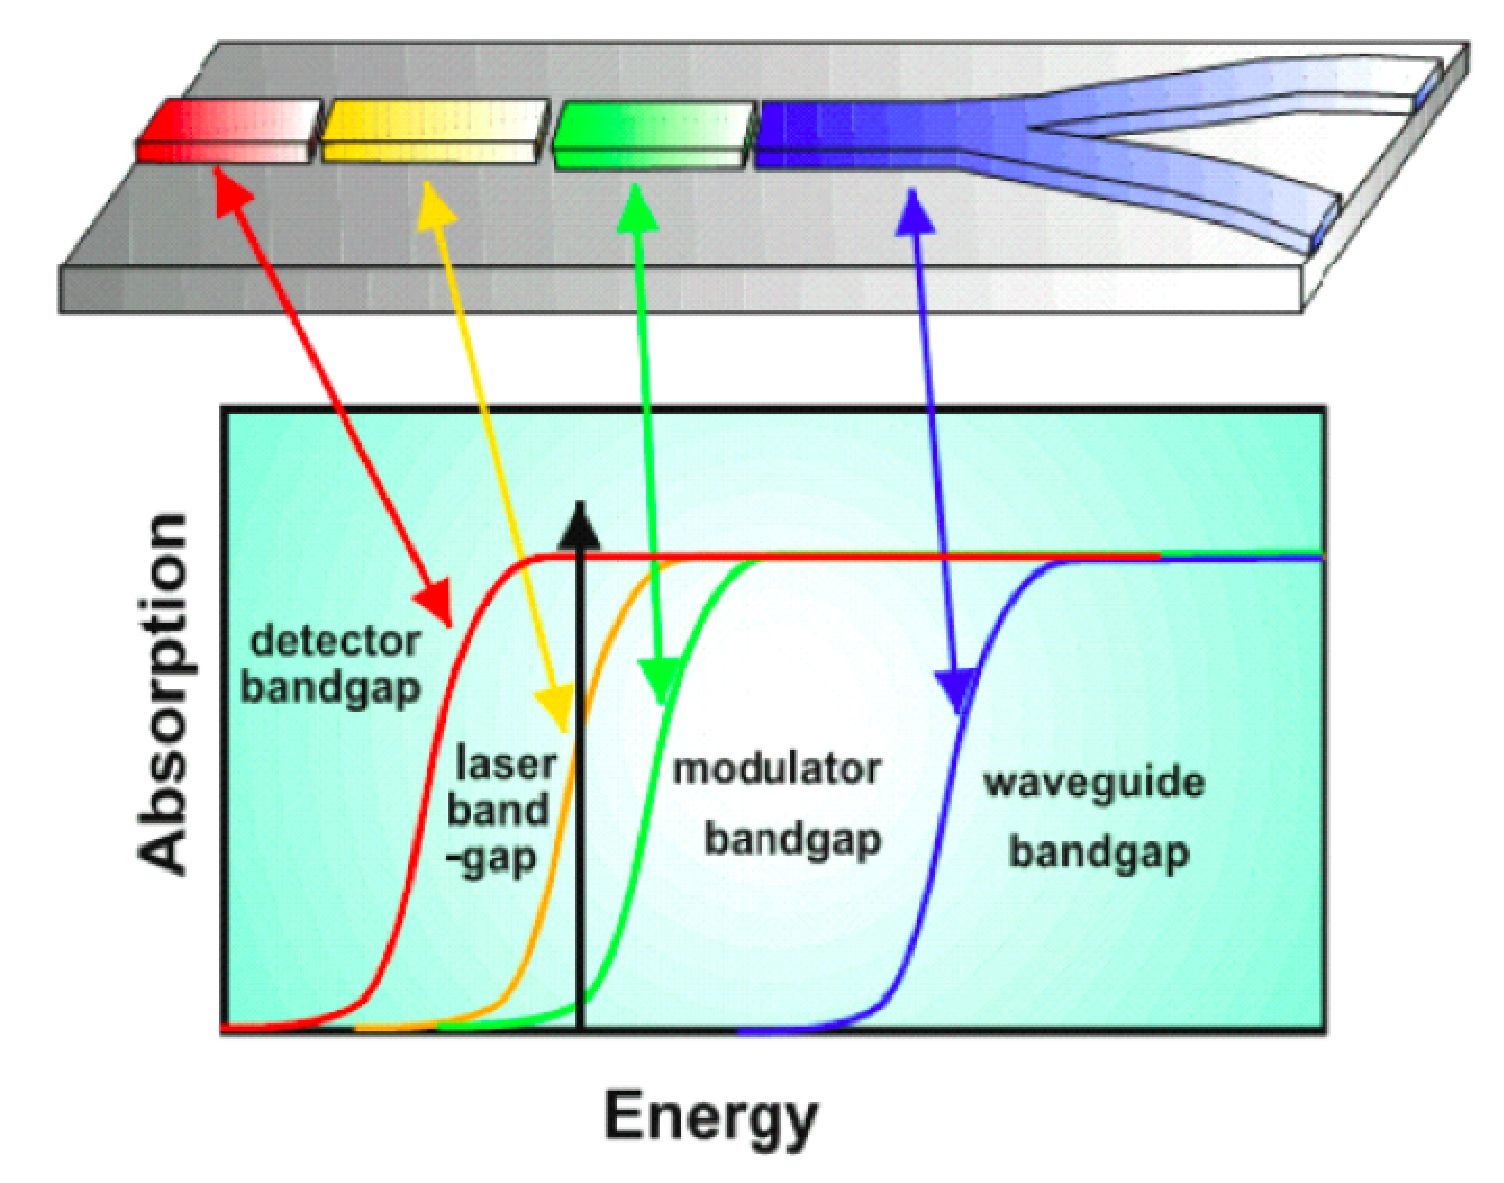
\includegraphics[width=0.7\textwidth]{./Pictures/pic.eps}\\
  \caption{光子集成回路示意图}
  \label{fig_pic}
\end{figure}

总的来说,任何一种单片集成的方法至少需要达到以下几条要求:

\begin{enumerate}
\item{精确的改变每个分立器件的材料的禁带宽度}
\item{空间分辨率应该远小于器件的尺寸}
\item{材料的其他特性不能变差太多,比如折射率、损耗、电特性等}
\end{enumerate}

%%%%%%%%%%%%%%%%%%%%
\section{单片集成技术的方法}
%%%%%%%%%%%%%%%%%%%%

为了在一块芯片上做出不同的禁带宽度,在过去的几十年中,已经有很多种方法实现这样的效果。然而,每一种方法都有他的优点和缺点,所以在实际生产中,还没有形成一种通常的解决方案,这也是该领域值得研究的一个问题。图\ref{fig_pic_methods}例举了几十年来人们所研究的各种单片集成方法。

\begin{figure}[!h]
  \centering
  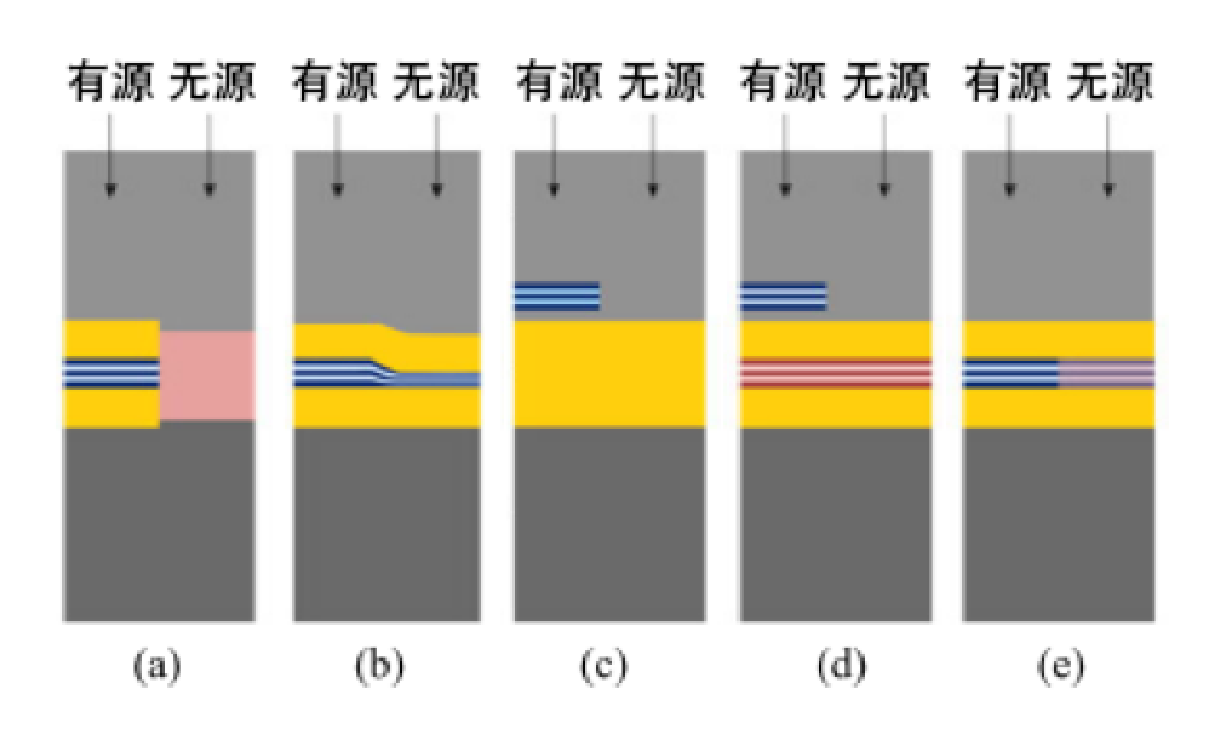
\includegraphics[width=0.7\textwidth]{./Pictures/pic_methods.eps}\\
  \caption{有源和无源器件单片集成的各种方法}
  \label{fig_pic_methods}
\end{figure}

%%%%%%%%%%%%%%%%%%%%
\subsection{对接再生长}
%%%%%%%%%%%%%%%%%%%%

对接再生长的方法如图 2.2(a)所示。这种方法的原理是,首先生长一片全部包含有源层的芯片,然后将无源部分的芯层刻蚀掉,最后在这些地方重新生长无源的芯层和包层。这种方法的优点是,每个部分的材料禁带宽度都可以非常准确的控制。同时,它的缺点也是显而易见的。由于有源的芯层和无源的芯层必须对准,而通常的量子阱片芯层仅有几十纳米,所以这给工艺带来了不小的难度。此外,如果需要制作多种不同禁带宽度的材料,就需要进行多次的刻蚀和再生长,大大增加了工艺的复杂度。最后,由于之后生长上去的材料和原先的材料完全不同,所以很可能存在较大的折射率差,这样会导致界面上的光被反射,增加了额外的损耗。近年来,很多人通过改进工艺,大大减小了界面的反射率,但是界面的质量依然是工艺上的难点。总而言之,这种方法最直接、最有效,同时在工艺上的难度和复杂度限制了它的发展。

%%%%%%%%%%%%%%%%%%%%
\subsection{选择性区域生长}
%%%%%%%%%%%%%%%%%%%%

选择性区域生长的方法如图 2.2(b)所示。这种方法只需要一步生长就可以完成,所以是对对接再生长的改进。这种方法的原理是,在芯片生长芯层之前,先在芯片上生长一层介质膜。然后,在用金属氧化物化学气相沉积(MOCVD)生长芯层的过程中,由于介质膜的影响,材料的厚度和组分会发生变化,导致禁带宽度的改变。只要介质膜生长得当,这种方法可以一次性生长出多个需要的禁带宽度的材料。不过,这种方法对MOCVD生长条件的控制非常苛刻,所以工艺难度非常高,同时器件的性能很容易受到表面状态的影响。

%%%%%%%%%%%%%%%%%%%%
\subsection{偏置量子阱}
%%%%%%%%%%%%%%%%%%%%

图 2.2(c)是偏置量子阱方法。这种方法的原理是,有源层的芯层被生长在无源层的芯层之上,最后在无源区域刻蚀掉有源层的芯层。这种方法比较简单直接,但是缺点似乎更多。首先,它只能将两种禁带宽度的器件集成在一起。然后,由于有源芯层不在最中间,激光器的限制因子会大大下降,这样会大大减小激光器的增益。最后,无源部分不包含量子阱层,所以在制作调制器时,性能会有所折扣。

%%%%%%%%%%%%%%%%%%%%
\subsection{双量子阱}
%%%%%%%%%%%%%%%%%%%%

图 2.2(d)是双量子阱方法。显然,该方法是偏置量子阱方法的改进。它在偏置量子阱的基础上,在无源芯层也生长了量子阱。这样可以解决调制器的性能问题。可是这种方法并不能解决偏置量子阱方法的其他问题,例如激光器限制因子仍然比较低等等。同时,由于无源区域包含量子阱层,损耗也要比偏置量子阱大很多。

%%%%%%%%%%%%%%%%%%%%
\subsection{量子阱混杂技术}
%%%%%%%%%%%%%%%%%%%%

从制作工艺的角度来说,图 2.2(e)所示的量子阱混杂技术可能是最简单的单片集成方法。如图 2.3所示,对于普通的量子阱材料来说,沿着材料的生长方向看过去,每一层材料的禁带宽度是一种矩形的结构。整个量子阱的禁带宽度是由阱的材料和厚度,以及垒的材料决定的。然后,当我们通过某种方法,将阱和垒的材料进行融合,使量子阱的每一层的禁带宽度变成一个渐变的结构之后,整个材料的禁带宽度就会发生变化(通常是禁带宽度增加)。所以,我们只需要在芯片生长完之后,制作各个部分的器件之前,对调制器和无源波导等区域进行量子阱混杂,其中禁带宽度的变化量由混杂的工艺参数决定,这样就可以实现单片集成的效果。

\begin{figure}[!h]
  \centering
  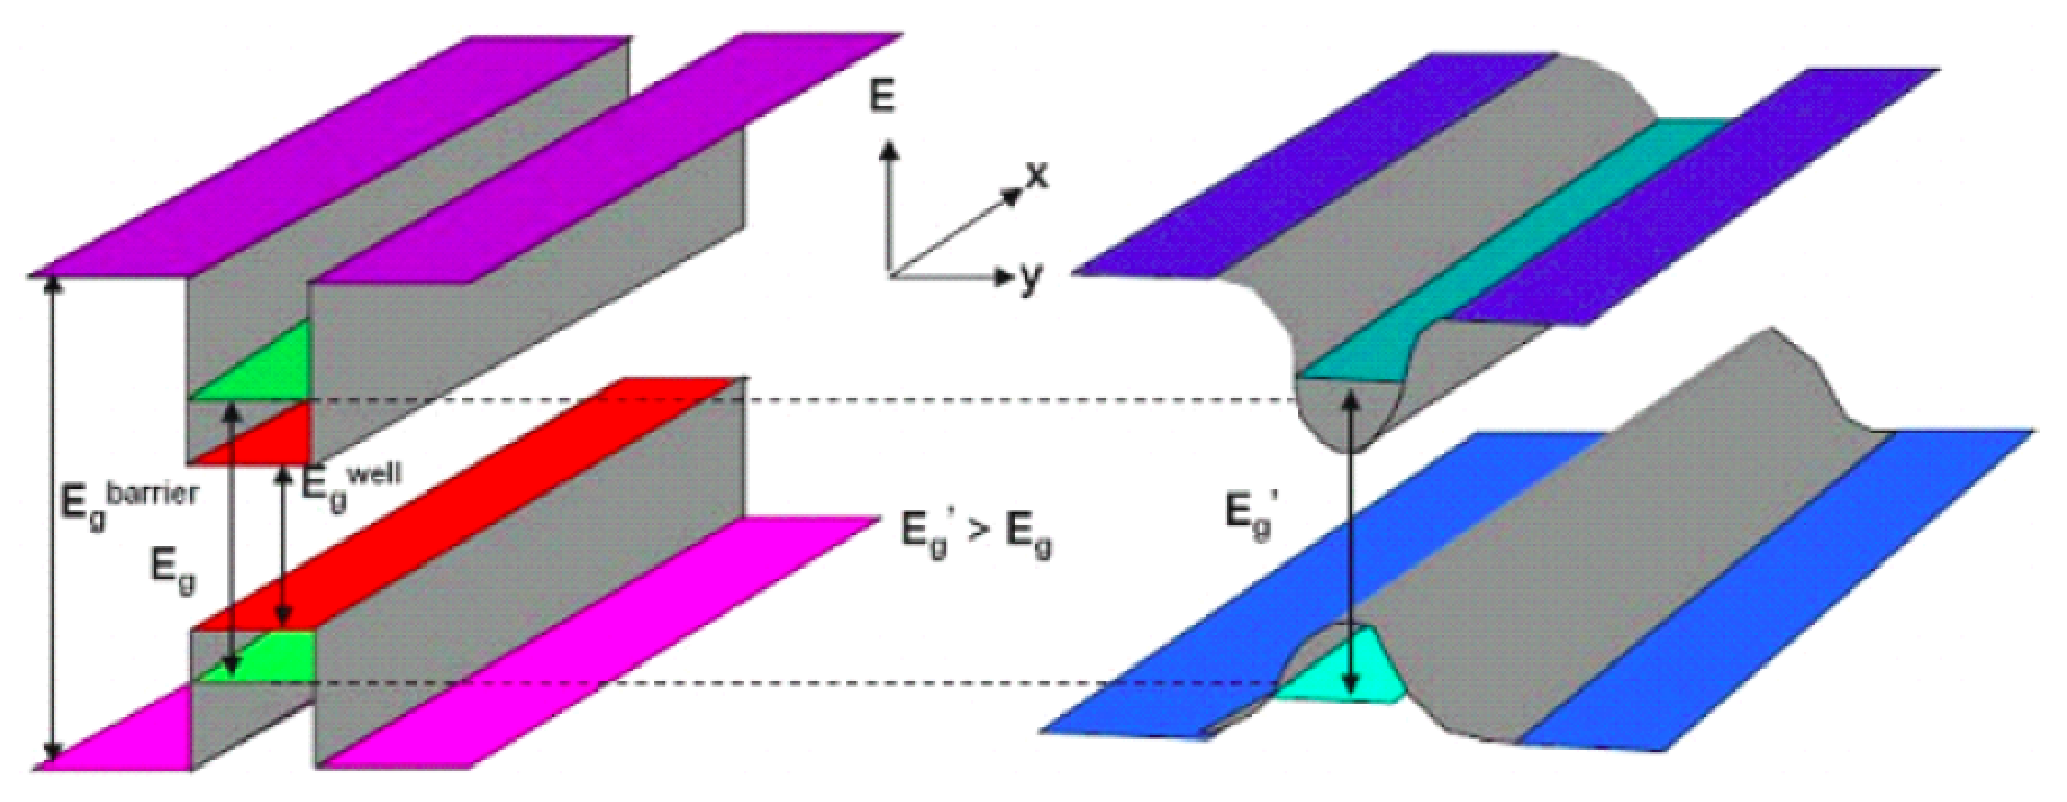
\includegraphics[width=0.7\textwidth]{./Pictures/qwi.eps}\\
  \caption{量子阱混杂技术示意图}
  \label{fig_qwi}
\end{figure}

为了让阱和垒互相融合,高温退火是最直接的方法。然而,只做退火的方法会引起一整片材料的禁带宽度变化,我们需要的是在特定的区域内改变材料的禁带宽度。所以通常会在芯片特定区域的表面或者内部产生一些缺陷。这些缺陷在快速退火的条件下,可以快速扩散到量子阱层,引起阱和垒互相扩散,达到量子阱混杂的目的。这些缺陷同时还能起到促进阱和垒互相扩散的目的,和单纯使用退火的方法相比,退火温度要低得多,退火时间要短得多。

除了快速热退火和引入的缺陷会影响量子阱混杂的效果之外,量子阱本身的结构也起到很大的作用。2009年,墨西哥INAOE研究院、瓜纳华托大学和美国佛罗里达大学共同发表了一篇关于InP量子阱结构对混杂的影响的文章[ ]。文章中采用了InGaAsP/InGaAsP、InGaAs/InGaAsP和InGaAs/InP三种不用的量子阱结构,在相同的实验条件下比较他们的混杂效果,如图 2.4所示。结果显示,量子阱的材料对蓝移的大小起了非常大的作用。InGaAs/InP量子阱因为阱和垒只有In原子是相同的,所以两种材料的差异最大,最容易达到量子阱混杂的效果。InGaAs/InGaAsP量子阱有In、Ga和As三种元素是共有的,所以混杂效果比前者差很多。而InGaAsP/InGaAsP的元素完全相同,只有组分不同,所以总体来说比InGaAs/InGaAsP量子阱的效果更差一些。

由于条件有限,我们在实验中采用的量子阱结构都是同一种,即InGaAsP/InGaAsP量子阱。 这是一个1.2\%压应变的应变五量子阱结构,激射波长在1550nm左右。从上到下,依次包含0.5μm厚的InP牺牲层,0.2μm厚的InGaAs盖层,1.5μm厚的InP上包层,0.004μm厚的InGaAsP阻刻层,渐变折射率层,五量子阱层,渐变折射率层,最下面是InP基片。在本文的后面篇章中,我们不会通过改进量子阱结构来提升量子阱混杂的效果。参考前面的讨论,InGaAsP/InGaAsP量子阱是相对来说效果最差的一个组合,这里还有很大的提升空间。

量子阱混杂的一个优点在于,该方法是在芯片外延之后进行的,所以只需要进行一次外延生长。该技术的具体实现方案通常是比较容易实现的,所以工艺复杂度比较低。此外,该方法制作的器件的性能也比较好。由于量子阱混杂之后,材料性能的变化很小,例如折射率基本不变,这样就不会在有源和无源区域的边界引入额外的损耗。该技术的缺点在于,具体的实现方案往往缺乏稳定性,在工艺参数发生微小变化的情况下,量子阱混杂的效果可能会发生较大变化。为了能得到稳定可靠的量子阱混杂技术,人们还在不断的创造和完善之中。

%%%%%%%%%%%%%%%%%%%%
\subsection{各种单片集成技术的比较}
%%%%%%%%%%%%%%%%%%%%

待添加。

%%%%%%%%%%%%%%%%%%%%
\section{量子阱混杂技术回顾}
%%%%%%%%%%%%%%%%%%%%

量子阱混杂是一个量子阱的阱和垒相互扩散的过程。在这个过程中,随着扩散的不断增强,量子阱的形状和厚度也随之不断变化,从而导致能带的变化。变化之后的能带对应的能量一般来说都是增加的,也就是波长发生蓝移。在一般情况下,量子阱的阱和势垒之间的界面是亚稳态的,在一定的条件下,例如高温下,量子阱的阱和势垒的原子会相互扩散。量子阱混杂的目标不是简单地使阱和势垒相互扩散,而是在整个区域中做选择性的扩散。

已经有很多种方法可以实现量子阱混杂的效果,例如杂质诱导无序(IID) \cite{holonyak1998impurity-IID} ,无杂质空位增强无序(IFVD) \cite{si1998area-IFVD},光吸收诱导无序(PAID) \cite{mckee1997monolithic-PAID},离子注入增强扩散\cite{charbonneau1998photonic-implantation}等等。本节将介绍最近几十年中研究过的绝大部分方法,并进行比较。

%%%%%%%%%%%%%%%%%%%%
\subsection{杂质诱导方法}
%%%%%%%%%%%%%%%%%%%%

\begin{figure}[!h]
  \centering
  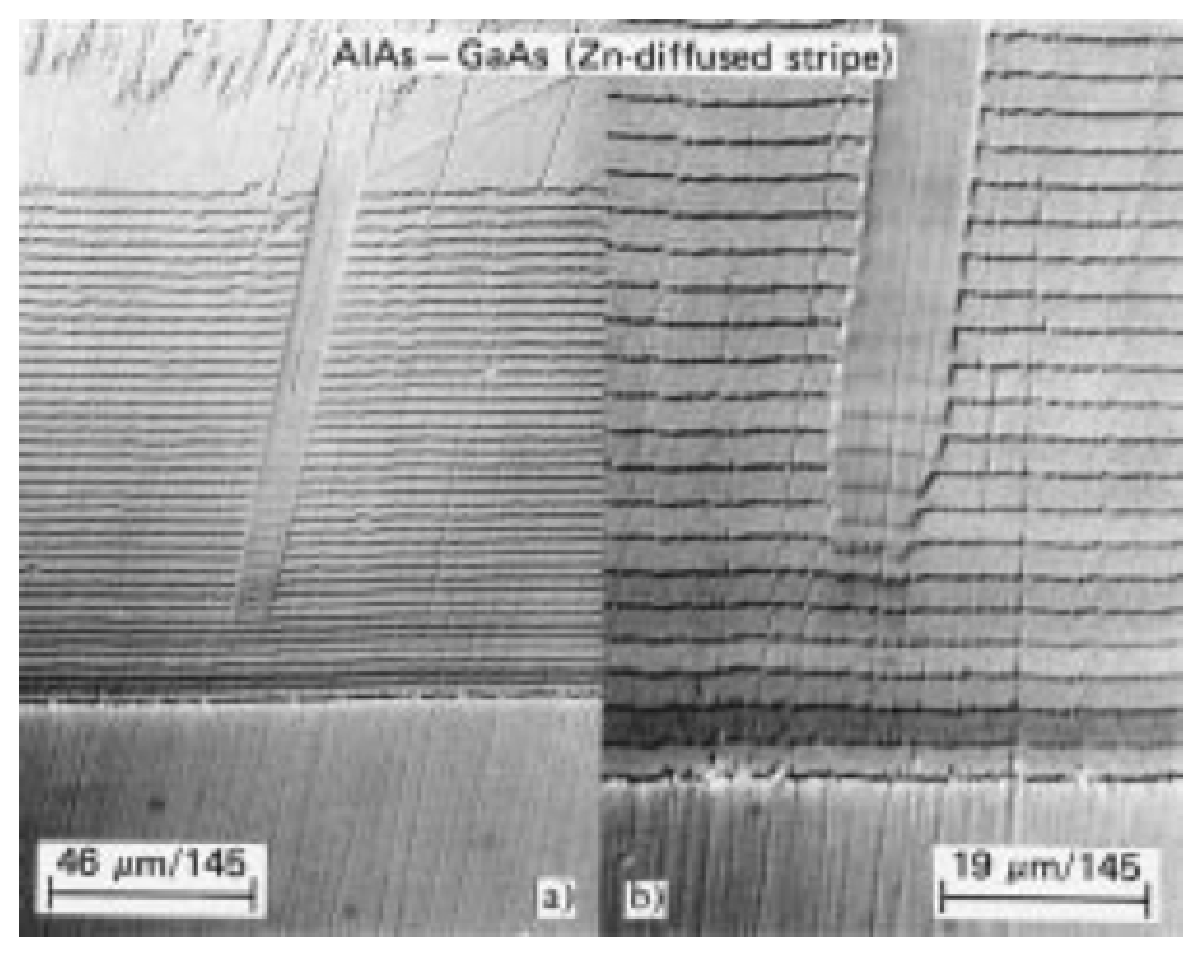
\includegraphics[width=0.7\textwidth]{./Pictures/iid.eps}\\
  \caption{Zn扩散到AlAs-GaAs超晶格中引起混杂的电镜图片}
  \label{fig_iid}
\end{figure}

19世纪80年代,人们开始研究量子阱混杂技术,第一个被想到和实现的是杂志诱导方法。1981年,美国伊利诺斯大学的W. D. Laidig等人提出了使用Zn扩散到AlAs-GaAs超晶格中引起混杂的方法\cite{laidig1981disorder},这也是第一次报道的杂质诱导方法(更详细的介绍可以参考一份相关的专利\cite{holonyak1983method})。如图\ref{fig_iid}所示,在AlAs-GaAs超晶格的中间10um区域,已经有Zn原子扩散到里面,扩散的温度仅仅需要575摄氏度,大大低于GaAs材料本身发生混杂的温度。在Zn扩散进去之后,AlAs-GaAs超晶格的组分发生了变化,变成了AlGaAs的三元合金,材料的禁带宽度也随之增加了。在这个实验中,为了达到Zn原子选择性扩散的目的,芯片表面利用光刻技术覆盖了一层Si3N4掩膜,然后和ZnAs2一起放入专门的扩散炉中,在500-600摄氏度的条件下等待10-60分钟,就可以在没有覆盖Si3N4的地方达到混杂的效果。

此后,人们在这篇文章的基础上,对杂质诱导方法进行了大量研究和改进。例如,美国罗克韦尔国际微电子研究发展中心的J. J. Coleman等人提出了用低能的Si离子注入实现AlAs-GaAs超晶格混杂的方法[ ]。他们使用375keV能量的Si离子,注入到AlAs-GaAs超晶格芯片的表面,然后在退火的作用下,达到了混杂的目的。此后,人们发现了Ge,S,Sn,Se,Be,Mg等原子也可以达到杂质诱导混杂的目的。1984年,美国麻省理工学院在InGaAsP量子阱材料上也实现了杂质诱导混杂的效果。他们用这种方法制作了10GHz的激光器和调制器集成的器件[ ]。然而,这种方法也有一些缺陷,比如电特性并不理想。由于量子阱混杂的过程中需要引入额外的杂质,这些杂质运动到芯片的接触层和上包层之后会使得电特性变差。所以这种方法并不是很适合制作一些复杂的有源器件。因此,人们探索了不使用额外杂质达到量子阱混杂目的的方法,后面介绍的方法都是属于不引入额外杂质的方法。

%%%%%%%%%%%%%%%%%%%%
\subsection{无杂质空位诱导方法}
%%%%%%%%%%%%%%%%%%%%

1986年,美国伊利诺斯大学的L. J. Guido等人发现了在GaAs量子阱材料表面的生长介质层会引起光谱蓝移的效果。他们是最早一批发现这种方法实现量子阱混杂的人。他们的实验过程是如图 2.6所示,首先在GaAs量子阱芯片的表面生长一层SiO2介质层,然后在800℃~900℃之间进行快速热退火。他们发现,GaAs表面的Ga原子由于在SiO2中扩散系数很大,所以会在快速热退火的过程中被吸附上去,这样就会在GaAs表面产生Ga空位。这些空位在随后的快速热退火会继续往下运动到量子阱层,促进阱和垒的扩散,达到量子阱混杂的目的。这种方法与前面的方法相比,由于不需要额外的杂质参与,所以理论上对材料的性能影响更小。同时介质层只需要利用普通的PECVD等设备就可以生长,这也是光器件的标准工艺步骤。

在GaAs量子阱材料上取得成功之后,人们尝试在InP量子阱材料上重复这个实验。由于必须有Ga原子的参与,介质层生长在InP牺牲层上面并不会达到量子阱混杂的目的,所以必须在InGaAs电接触层上生长。不过这并不是这个方法的真正难点。难点在于,为了将Ga原子吸附到介质层中,必须采用较高的退火温度,通常在800℃以上。这个温度条件小于GaAs量子阱本身混杂的温度,但是大于InP量子阱本身混杂的温度。其中的一个比较通用的解决办法例如在2002年,J. H. Teng等人提出了利用生长SixNy介质层抑制高温退火带来的蓝移的技术[ ],结果如图 2.7所示。对于生长SiO2的样品,PL波长峰值蓝移到了1390nm左右,这个蓝移效果是比较理想的。但是,没有介质层的裸片退火之后波长在1500nm附近,相对于原生片的1575nm蓝移了75nm,这个蓝移明显太大。而生长SixNy部分的蓝移减小到了50nm以下,明显对混杂起到了抑制作用。他们用这种方法制作了延长腔激光器,达到了10nm的电调谐范围,这个结果是很理想的。

总的来说,这种方法更适合于GaAs量子阱材料,可以说是GaAs量子阱混杂的最佳选择。然而在InP量子阱材料上,需要额外生长抑制蓝移的介质层,给工艺带来了很大的复杂性。所以该技术并不太适合InP量子阱材料。值得一提的是,利用这项关键技术,英国格拉斯哥大学的John H. Marsh教授创办了Intense公司,专门生产大功率GaAs半导体激光器。对于GaAs量子阱激光器来说,由于量子阱中Al元素的存在,当注入电流比较大的时候,激光器的端面会突然发生烧毁的现象,导致整个激光器失效。这个现象成为光学灾变(COD)[ ]。所以GaAs量子阱激光器往往不能输出很大的功率。解决这个问题的一个巧妙的办法就是将靠近解理面部分的材料变成无源材料,形成一个非吸收腔镜(NAM),这样可以很大程度上抑制光学灾变现象的发生[ ],从而提高了GaAs激光器的功率。这也是量子阱混杂技术在激光器中的一个巧妙的应用。

%%%%%%%%%%%%%%%%%%%%
\subsection{低温生长InP方法}
%%%%%%%%%%%%%%%%%%%%

2000年,加拿大McMaster大学的David Thompson等人提出了一种在InP量子阱芯片上利用低温生长InP和快速热退火实现量子阱混杂的方法[ , ]。其中的关键技术在于,他们把量子阱芯片的InP牺牲层的生长温度从470℃下降到300℃,这样可以在牺牲层中引入缺陷。这些缺陷在之后的快速热退火中会往下运动,促进阱和垒的混杂,达到禁带宽度蓝移的目的。图 2.8给出了常温和低温InP层在725℃快速热退火条件下产生的蓝移随着退火时间的变化趋势。显而易见的是,常温InP层并不会对量子阱混杂达到促进作用,而低温InP层大大促进了量子阱混杂,并且蓝移可以达到170nm以上。

该课题组在之后的时间里继续探索了这种技术的一些细节问题,包括利用x射线分析量子阱混杂之后的样品组分[ ],研究低温生长InP的温度、P流量和厚度对量子阱混杂的影响[ ],利用XTEM和EDX技术分析量子阱混杂之后的样品组分[ ],同时衍生出了利用He辅助生长InP[ ]和生长InAsP[ ]的技术实现量子阱混杂的方法。然而,这种技术并没有往更深的方向发展。由于低温生长InP的工艺本身并不是标准工艺,所以他的可重复性是存在问题的。至今并没有其他的第二个课题组重复过这种技术。他们也没有进一步利用这种技术制作器件。

%%%%%%%%%%%%%%%%%%%%
\subsection{阳极氧化诱导方法}
%%%%%%%%%%%%%%%%%%%%

1998年,香港大学的Shu Yuan等人提出了一种在GaAs量子阱芯片上采用阳极氧化实现量子阱混杂的方法\cite{yuan1998anodic}\cite{yuan1998anodicJSTQE}。其工艺设备如图\ref{fig_oxide}所示。首先,GaAs量子阱片被固定在一个开路的50伏脉冲式电源的阳极上。阳极和阴极之间通过导电液传到电流。导电液由乙二醇、磷酸和去离子水用40:20:1的体积比配制而成。芯片的一半由导热胶覆盖,这样一来,只有另一半暴露在导电液中的部分会被氧化。经过几分钟的脉冲电流处理之后,芯片又进行了快速退火处理。最终的测试结果如图\ref{fig_oxide_pl}所示。在芯片没有被氧化的部分,光致发光谱的峰值波长仅仅蓝移了5meV左右,同时强度下降到只剩原来的1/20。而对于氧化过的部分,蓝移达到了44meV,而强度上升到了原来的两倍多。可见,这种方法在获得较大蓝移的同时,还可以增加光致发光谱的强度。

\begin{figure}[!h]
  \centering
  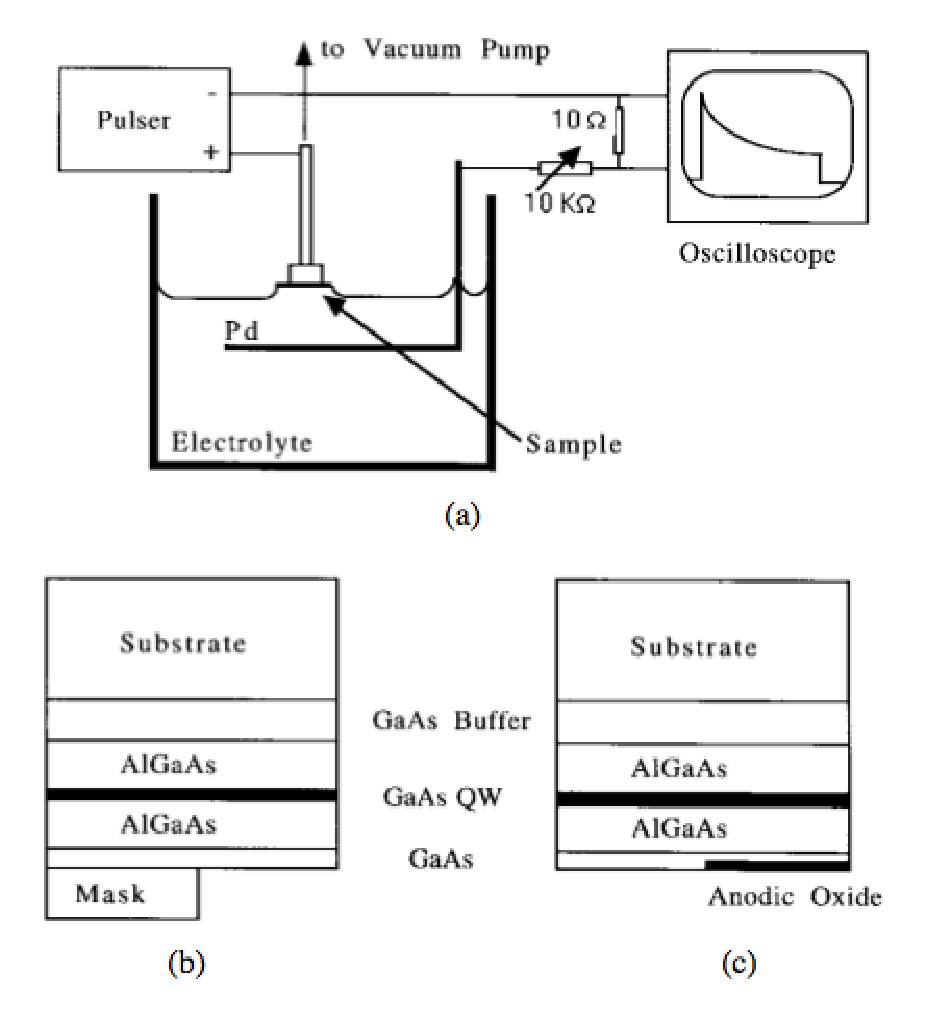
\includegraphics[width=0.7\textwidth]{./Pictures/oxide.eps}\\
  \caption{阳极氧化诱导量子阱混杂技术的设备示意图}
  \label{fig_oxide}
\end{figure}

\begin{figure}[!h]
  \centering
  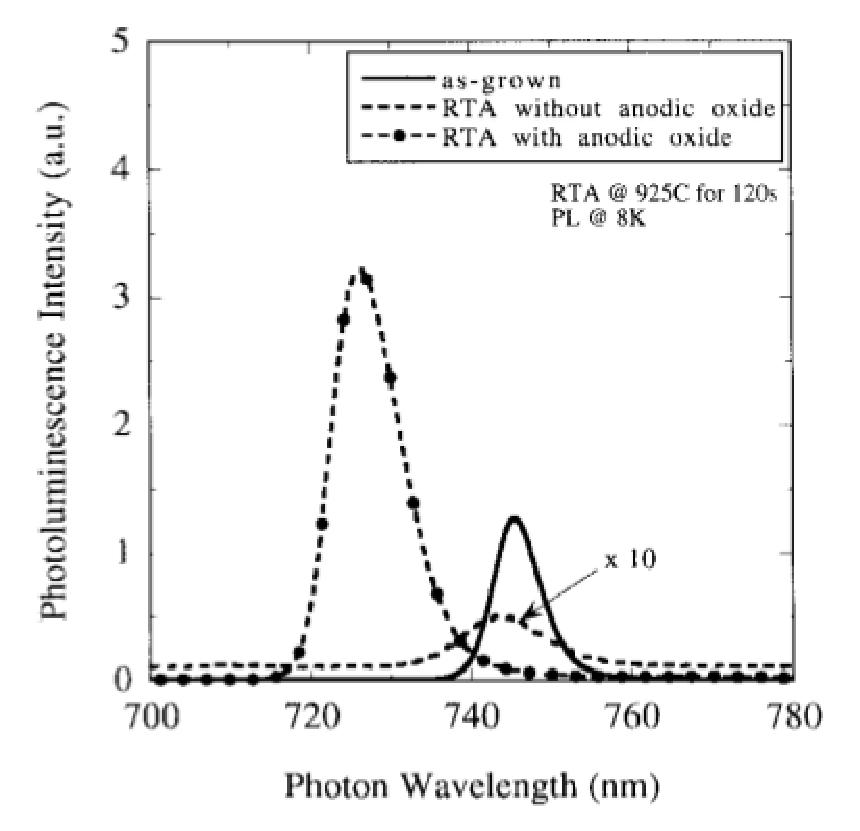
\includegraphics[width=0.7\textwidth]{./Pictures/oxide_pl.eps}\\
  \caption{混杂前后的光致发光谱测试结果}
  \label{fig_oxide_pl}
\end{figure}

可惜的是,这种方法由于需要非常特殊的实验条件,后来并没有进行广泛研究。这种方法也只能停留在研究光致发光谱蓝移的方向上,并没有应用到任何器件上,也没有在InP量子阱材料上成功实现。

%%%%%%%%%%%%%%%%%%%%
\subsection{光吸收诱导方法}
%%%%%%%%%%%%%%%%%%%%

1997年,英国格拉斯哥大学的Andrew McKee等人提出了用激光照射实现量子阱混杂的方法\cite{mckee1997monolithic-PAID}。该方法使用Nd:YAG激光器照射芯片的表面。由于Nd:YAG激光器发出的光波长在1064nm左右,介于InP的波长和芯层1550nm波长之间,所以正好可以穿过InP包层直接被芯层吸收,达到类似于加热退火的作用。整个工艺的过程是这样的。首先,芯片的表面会生长一层500nm厚的二氧化硅,既可以作为减反射薄膜,又可以对芯片表面原子起到一定的保护作用。然后,芯片被放在200摄氏度的热盘上,这样既可以提供一个背景温度,减小了Nd:YAG激光器照射所需的能量,又可以防止加热后的芯片过快地将热量往下散发。最后,Nd:YAG激光器输出$5W/mm^2$的光,照射芯片30分钟。该方法可以得到最大160nm的蓝移,这是相当可观的,同时还能保持材料的优良性能。混杂之后的激光器,计算得到的损耗甚至比混杂之前的还要小,这说明该方法不会增加甚至减小材料的损耗。由这种方法制作的无源波导,损耗仅有$5dB/cm$。

虽然这种方法效果很好,但是这种方法的致命缺陷在于,长时间的照射会让空间分辨率变得很差。2004年,美国利哈伊大学的Boon Siew Ooi等人提出了采用脉冲光吸收的新方法\cite{ooi2004multiple}。该方法采用一个Q调制的Nd:YAG激光器(10Hz,2.8-3.9$mJ/mm^2$,1-10分钟)照射芯片,然后再进行快速退火(625摄氏度,120秒)的方法。显然这种方法与采用连续Nd:YAG激光器照射的方法相比,原理是不同的。虽然波长一样,但是它产生的光只能被芯片表层的InGaAs吸收,并且在它的表面产生缺陷。这层缺陷在之后的快速退火中往下扩散,达到混杂的目的。这种方法制作的芯片除了有连续激光器照射方法的优点之外,其空间分辨率达到了2.5um,完全达到了单片集成的要求。

%%%%%%%%%%%%%%%%%%%%
\subsection{等离子体轰击方法}
%%%%%%%%%%%%%%%%%%%%

2002年,新加坡南阳理工大学的Ting Mei教授团队提出了用等离子体刻蚀机和快速退火实现量子阱混杂的方法[ ]。该方法首先利用等离子体刻蚀机形成的氩气等离子体轰击芯片的表面,形成一层非常薄(约10nm)的缺陷层。然后,在快速退火的作用下,这层缺陷往下扩散到量子阱层,促进量子阱的阱和垒的互相融合,达到量子阱混杂的目的。与其他的方法相比,这种方法最大的优点在于,不需要为了量子阱混杂购买额外的设备,因为等离子体刻蚀机是刻蚀芯片必须的设备,而快速退火也会在制作电极的欧姆接触时用到。而且,其工艺步骤非常简单,只需要等离子体轰击和快速退火两步就可以完成。如果需要对芯片做选择性的量子阱混杂,只需要在不做混杂的区域覆盖一层光刻胶或者二氧化硅掩膜,用来阻挡氩气等离子体的轰击就可以实现。2005年,该团队报道了利用这个方法制作的延长腔激光器[ ],也是至今为止唯一报道的用等离子体轰击方法制作的有源和无源单片集成的器件。通过研究延长腔激光器和全有源激光器的性能对比,可以估算出无源波导的损耗在10dB/cm左右。此外,很有意思的是,他们还发现了芯片表面的掺杂情况会对量子阱混杂的效果产生很大影响[ ]。

虽然这种方法具有工艺简单,成本低,效果好等优点,并且已经有了延长腔激光器这样的简单的集成应用,但是人们发现它的可重复性存在很大的问题。2011年,浙江大学的彭盛华硕士等人重复了上面的实验[ ],其中所用的等离子体刻蚀机与南阳理工大学的刻蚀机是同一型号的(Oxford ICP 100)。在类似的工艺参数条件下(ICP功率500w,RF功率480w,ICP处理时间1分钟,ICP温度20度,Ar流量80sccm,退火温度750℃,退火时间2分钟)他们发现,尽管材料的禁带宽度也可以蓝移100nm以上,但是光致发光谱的强度下降了一半左右,如图 2.11所示。当他们把氩气等离子体换成氮气之后,同样发现在得到大蓝移的同时,光致发光谱下降了很多[ ],如图 2.12所示。用这种方法制作的无源波导测试得到的损耗如图 2.13所示,达到了68dB/cm[ ],完全达不到无源器件集成的要求。所以,这种方法只有在蓝移50nm左右的情况下可以做得较好。或者在没有上包层的芯片上做,然后再生长上包层,这样又大大增加了工艺的复杂度。总的来说,用等离子体轰击方法实现量子阱混杂的方法还有待进一步的研究。

%%%%%%%%%%%%%%%%%%%%
\subsection{溅射轰击方法}
%%%%%%%%%%%%%%%%%%%%

溅射轰击方法与等离子体轰击方法的原理有些相似。首先,芯片在溅射的过程中,在表面产生一层很薄的缺陷层。然后,这层缺陷在快速退火的条件下快速运动到量子阱区域,促进阱和垒的互相扩散,达到量子阱混杂的目的。这种方法也不需要购买额外的设备,因为溅射机是制作激光器电极的设备。如果需要对芯片做选择性的量子阱混杂,只需要在不做混杂的区域覆盖一层光刻胶或者二氧化硅掩膜,这些特点与等离子体轰击方法完全相同。不同的地方在于溅射的靶的材料。1998年,英国格拉斯哥大学的John Marsh教授团队提出了利用溅射SiO2和快速退火的方法实现量子阱混杂的效果[ ]。值得一提的是,如果SiO2溅射在含有Ga原子的材料表面,就可能发生前面讨论的无杂质空位诱导的现象。所以在重复这个实验时,需要区分这两种现象,因为他们的原理是完全不同的。

在2014年,浙江大学的朱洪力等提出了溅射氧化铝[ ]和氮化硅[ ]实现量子阱混杂的技术。在他们的实验中,经过溅射和快速热退火处理之后的InP量子阱片可以蓝移100nm以上,如图 2.14。而混杂之后的波导损耗下降到了18dB/cm,如图 2.15所示,这些都是比较理想的结果。

%%%%%%%%%%%%%%%%%%%%
\subsection{离子注入方法}
%%%%%%%%%%%%%%%%%%%%

离子注入方法由离子注入和快速退火两个步骤组成。首先,特定种类的离子在非常高能量的离子注入机的加速下,直接打入芯片的内部。然后,在快速退火的作用下,这些离子促进了量子阱中的阱和垒的融合,最终达到改变禁带宽度的目的。

\begin{figure}[!h]
  \centering
  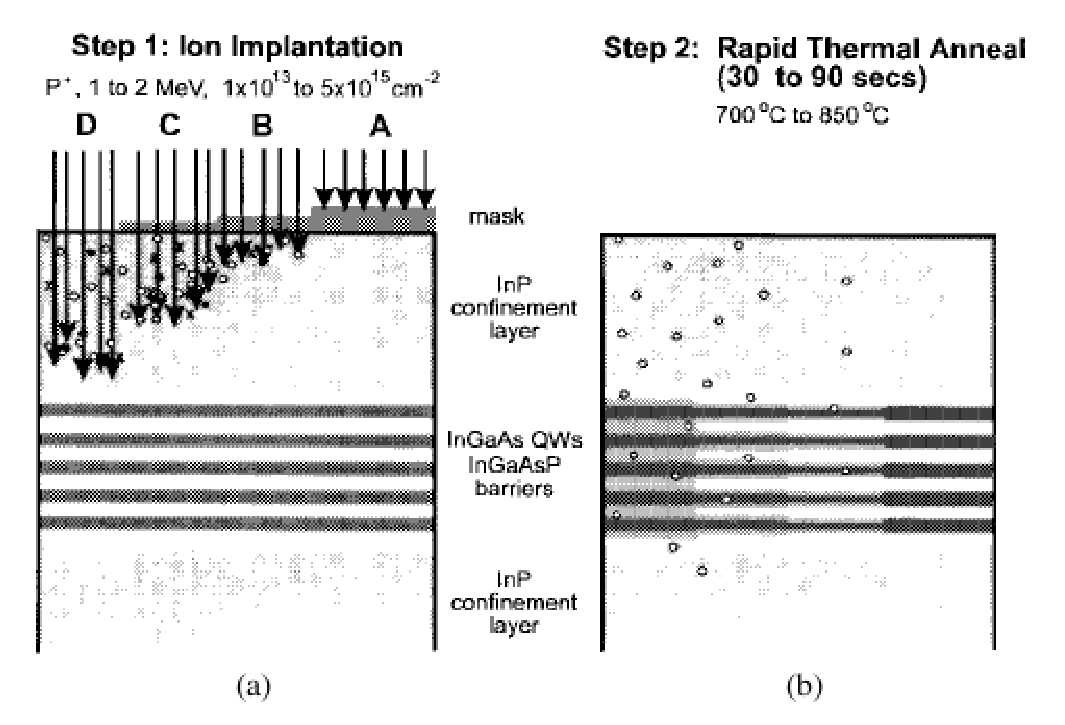
\includegraphics[width=0.7\textwidth]{./Pictures/implantation.eps}\\
  \caption{离子注入技术示意图}
  \label{fig_implantation}
\end{figure}

如图\ref{fig_implantation}所示,在D区域,磷离子在离子注入机的加速下直接注入到芯片的上包层,并在之后的快速退火的作用下,促进量子阱的阱和垒的互相融合。最有意思的是,在C、B、A区域,芯片表面生长了一层$SiO_2$掩膜。这层掩膜可以抵消一部分离子注入的能量,导致离子只能注入到稍浅的地方,最终这些区域的量子阱混杂程度会比没有掩膜的地方稍弱。通过制作不同厚度的$SiO_2$掩膜,就可以精确地控制量子阱混杂的程度,并且只需要一次快速退火就可以形成很多个不同禁带宽度的区域。

离子注入方法制作的无源波导的性能甚至比量子阱混杂之前的性能还要好。如图\ref{fig_implantation_wg_test}所示,量子阱混杂之后,波导的禁带宽度相比于未混杂的波导,蓝移了90nm左右。计算得到的损耗如图\ref{fig_implantation_wg_loss}所示。对于未混杂的波导,在透明传输的波长区域,比如1580nm,波导的损耗大约是$8cm^{-1}$。对应到混杂之后的波导的1490nm,波导的损耗只有$5cm^{-1}$左右。也就是说,经过离子注入方法制作的无源波导,损耗可以比未做处理之前还要低。

\begin{figure}[!h]
  \centering
  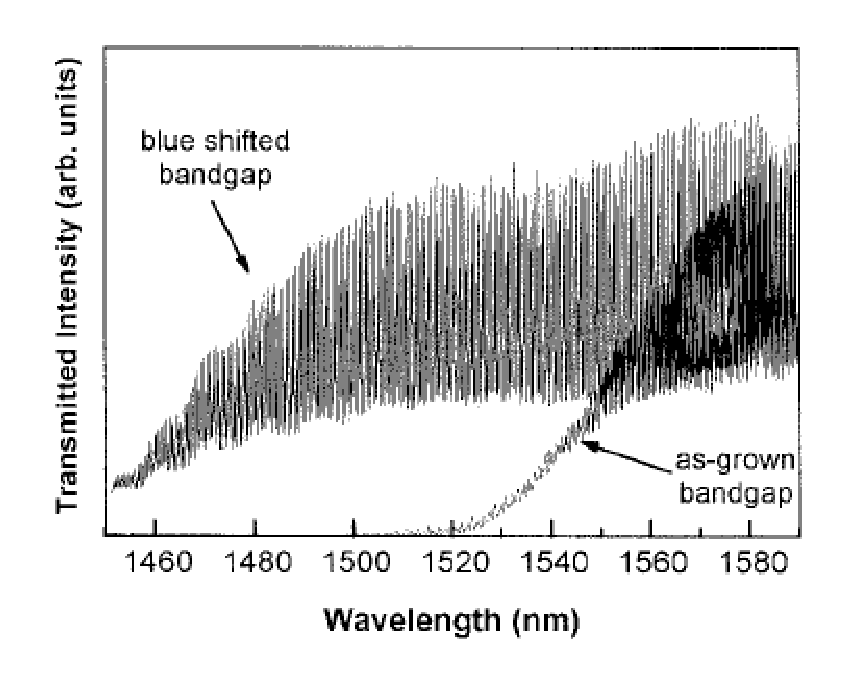
\includegraphics[width=0.7\textwidth]{./Pictures/implantation_wg_test.eps}\\
  \caption{测试得到的量子阱混杂和未混杂波导的透射光谱}
  \label{fig_implantation_wg_test}
\end{figure}

\begin{figure}[!h]
  \centering
  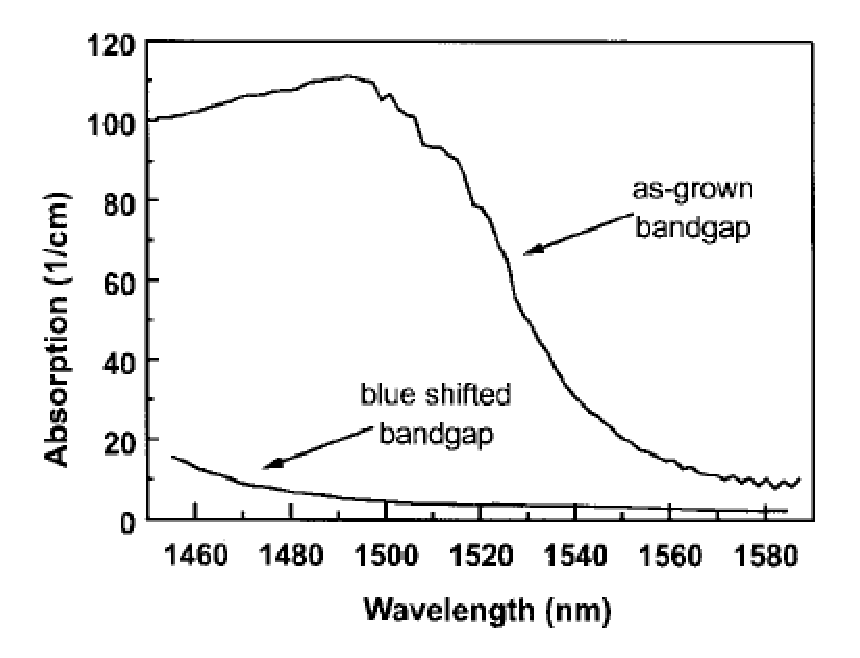
\includegraphics[width=0.7\textwidth]{./Pictures/implantation_wg_loss.eps}\\
  \caption{由透射光谱计算得到的损耗}
  \label{fig_implantation_wg_loss}
\end{figure}

利用离子注入技术制作的激光器的IV特性曲线如图\ref{fig_implantation_laser}所示。从图中可以看出,在量子阱混杂前后,两种激光器的IV曲线是非常相似的。在激光器工作的第一象限,两条曲线基本重合在一起。这说明,离子注入技术不会改变材料的电特性。

\begin{figure}[!h]
  \centering
  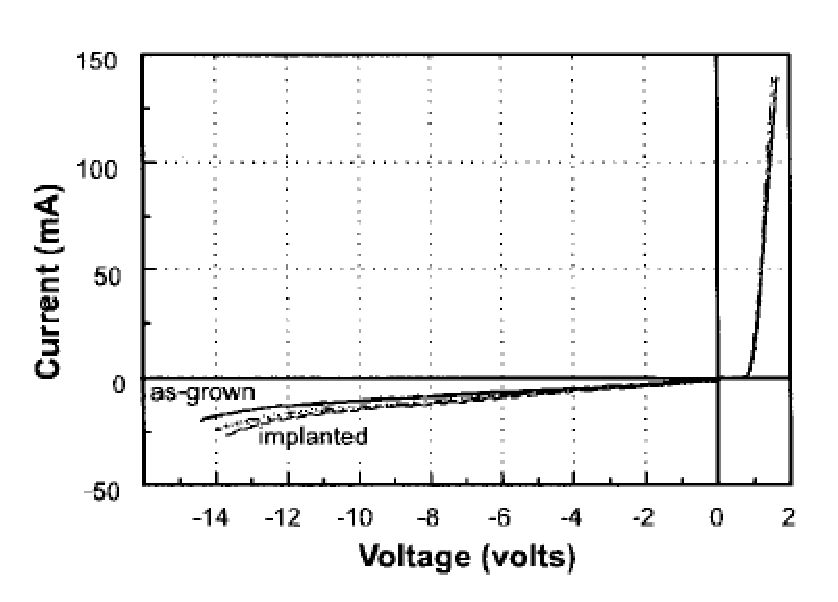
\includegraphics[width=0.7\textwidth]{./Pictures/implantation_laser.eps}\\
  \caption{由离子注入方法制作的激光器的IV特性曲线}
  \label{fig_implantation_laser}
\end{figure}

由于离子注入技术相对成熟,性能也很好,人们已经利用该技术制作了非常复杂的单片集成器件。第一章中介绍的Larry Coldren教授制作的8×8单片集成可调谐光路由器就是才采用了这个技术。

除了通常的高能离子注入方法之外,人们也尝试了高能聚焦离子注入机(FIB)实现量子阱混杂的方法。1998年,德国维尔兹堡大学的Johann Peter Reithmaier和Alfred Forchel提出了利用高能聚焦离子注入机实现量子阱混杂的方法[ ]。原理上,他和普通的离子注入方法是完全一样的,所以他也有离子注入方法的大部分优势。不同的是他的处理面积很小,通常在纳米量级,这样可以用来制作增益耦合DFB激光器的光栅结构。当然由于离子束太小,当加工大范围的区域时,就显得太费时费力了。

%%%%%%%%%%%%%%%%%%%%
\subsection{各种量子阱混杂方法的比较}
%%%%%%%%%%%%%%%%%%%%

待添加。

%%%%%%%%%%%%%%%%%%%%
%%%%%%%%%%%%%%%%%%%%
\chapter{量子阱混杂技术的理论模拟}
%%%%%%%%%%%%%%%%%%%%

在量子阱混杂工艺研究不断取得进展的同时,人们也做了很多量子阱混杂的理论模拟方面的工作。这些模拟让人们更好地理解了量子阱混杂的机理,并指导人们在工艺上进一步优化。量子阱混杂的理论模拟最核心的问题是计算混杂之后的能带结构。也就是说,在原有的量子阱的基础上,通过加入混杂的工艺参数作为变量,计算得到混杂之后的能带结构。有了能带结构之后,就可以进一步计算材料的吸收系数,增益,折射率等等。最后,就可以计算出量子阱混杂对整个光器件的影响。这一章将详细介绍量子阱混杂的能带结构的计算方法。

%%%%%%%%%%%%%%%%%%%%
\section{薛定谔方程的数值解法}
%%%%%%%%%%%%%%%%%%%%

在半导体中,电子运动的状态可以通过解薛定谔方程得到。

\begin{equation}
    \label{schrodinger}
    \frac{-h^2}{2} \frac{d}{dz} \frac{1}{m_\perp^*(z)} \frac{d\varphi(z)}{dz}
    +V(z)\varphi(z)
        = E\varphi(z)
\end{equation}

其中,$m_\perp(z)$是电子或者空穴的有效质量。$V(z)$是导带或者价带的势函数。(需要结合量子力学的课本重写)

然后,我们采用包络函数近似对上面的方程进行简化。在这个近似中,波函数的时间和空间分量可以分离开来,得到如下的函数式

其中??是波函数的稳态解,E是能量特征值。接着,我们还需要用有效质量近似再对薛定谔方程做一次简化,并且写成一维方向上的函数式,最后可以写成

\begin{equation}
    \label{eq_effective_mass}
    \left[ \frac{-\hbar^2}{2} \frac{d}{dx} \frac{1}{m^*(x)} + V(x) \right] \psi(x) = E \psi(x)
\end{equation}

我们只需要知道有效质量$m^*(x)$和势能$V(x)$在每个x上的值,就可以求出整个系统的特征值和特征函数,对应半导体能级的能量$E$和波函数$\psi(x)$。求解上述方程的数值方法有很多,包括有限差分法、传输矩阵法和有限元法等等。我们选择了相对简单,并且精度足够用的传输矩阵法。首先,我们需要将上面方程中的势函数和有效质量进行离散化,如图\ref{fig_tmm}所示。在每一小段的离散区间内,势函数和有效质量被视为不变,也就是说,在$x_j\le x<x_j+\Delta_j=x_{j+1}$时,$V_j=V(x_j)$,$m^*_j=m^*(x_j)$,而在这一段的末尾进行$V_j\to V_{j+1}$,$m^*_j\to m^*_{j+1}$的跳变。在$x_j\le x<x_{j+1}$的区间内,方程\ref{eq_effective_mass}的解可以表示为

\begin{equation}
    \label{eq_effective_mass_solution}
    \psi(x) = A_j \exp [i k_j (x-x_j)] + B_j \exp [-i k_j (x-x_j)]
\end{equation}

\begin{figure}[!h]
  \centering
  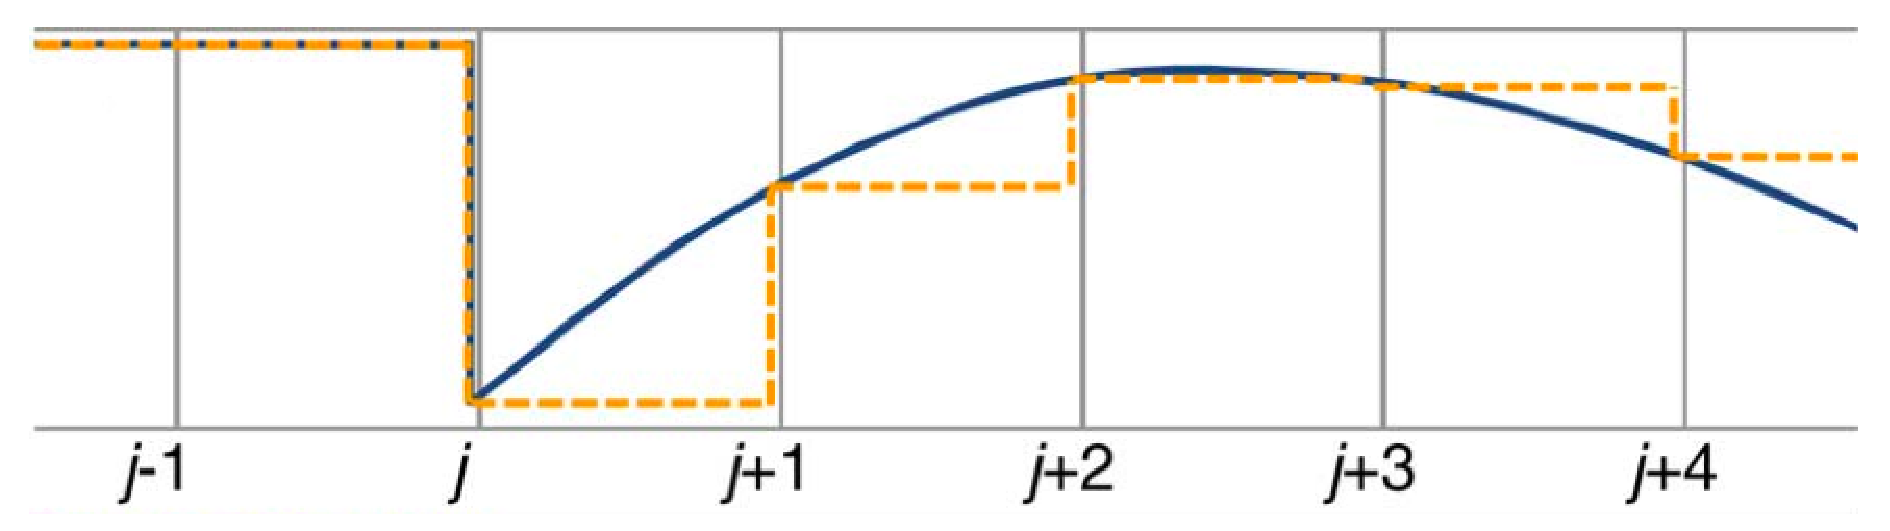
\includegraphics[width=0.7\textwidth]{./Pictures/tmm.eps}\\
  \caption{传输矩阵法对势函数和有效质量的离散化,实线代表精确值,虚线代表离散值}
  \label{fig_tmm}
\end{figure}

其中$k_j=\sqrt{2 m^*_j (E-V_j)} / \hbar$是波函数的波数。同时,方程\ref{eq_effective_mass}的边界条件需要满足波函数和它的导数在每个区间的连接点上连续,即如下两个方程

\begin{equation}
    \label{eq_boundary_1}
    \psi_{j-1}(x_{j-1}) = \psi_j(x_{j-1}) 
\end{equation}

\begin{equation}
    \label{eq_boundary_2}
    \frac{1}{m^*_{j-1}} \frac{d}{dx} [ \psi_{j-1}(x_{j-1}) ] = \frac{1}{m^*_j} \frac{d}{dx} [\psi_j(x_{j-1})]
\end{equation}

将边界条件方程\ref{eq_boundary_1}和\ref{eq_boundary_2}代入方程\ref{eq_effective_mass},就可以得到相邻两层的波函数振幅之间的关系,即

\begin{equation}
    \label{eq_tmm}
    \begin{pmatrix} A_{j+1} \\ B_{j+1} \end{pmatrix} = T_{j,j+1} \begin{pmatrix} A_{j} \\ B_{j} \end{pmatrix}
\end{equation}

其中的传输矩阵为

\begin{equation}
    \label{eq_transfer_matrix}
    T_{j,j+1} = \frac{1}{2\beta_{j+1}} \begin{pmatrix} \beta_{j+1}+\beta_j & \beta_{j+1}-\beta_j  \\ \beta_{j+1}-\beta_j  & \beta_{j+1}+\beta_j  \end{pmatrix} \begin{pmatrix} e^{ik_j\Delta_j} & 0 \\ 0 & e^{-ik_j\Delta_j} \end{pmatrix}
\end{equation}

其中$\beta_j = k_j/m^*_j$。最后,我们可以将每一层的传输矩阵从左往右连续相乘,得到如下的方程

\begin{equation}
    \label{eq_tmm_serial}
    \begin{pmatrix} A_{N} \\ B_{N} \end{pmatrix} = T_{N-1,N}T_{N-2,N-1}\cdots T_{0,1} \begin{pmatrix} A_{0} \\ B_{0} \end{pmatrix} =  \begin{pmatrix} T_{11} & T_{12} \\ T_{21} & T_{22} \end{pmatrix} \begin{pmatrix} A_{0} \\ B_{0} \end{pmatrix}
\end{equation}

其中$N$是分段的总段数。这个连续的方程需要满足收敛条件,也就是$A_0=B_N=0$,对应于最后的方程

\begin{equation}
    \label{eq_t22}
    T_{22}=0
\end{equation}

上面的方程是一个关于E的复数方程,它的所有解,从小到大依次就是每一个能级,代入到前面的波动方程\ref{eq_effective_mass_solution}中,就可以得到每个x点上的波函数。

为了验证程序的正确性,我们选择了文献中的AlGaAs-GaAs量子阱结构\cite{jonsson1990solving},其势能和有效质量如表\ref{tmm_sample}所示。由于导带和价带的能级计算方法完全一样,这里只给出导带的计算结果,如表所示。我们将文献中的传输矩阵法\cite{jonsson1990solving}、有限元法\cite{nakamura1989finite}的结果和我们的结果作比较,发现结果基本上是一致的,误差最大仅有0.03\%,说明了该程序是正确的。存在的一些微小偏差主要来源于对x轴的取值不同。x轴的离散化的步长和整个x轴的长度,会对能级的结果产生细微的影响。此外,我们还计算了前四个能级对应的波函数振幅的平方,并且与势函数叠加在一起,如图\ref{fig_waves}所示。结果再一次验证了程序的正确性。

\begin{table}[!t]
    \zihao{5}
    \caption{用于传输矩阵法计算的AlGaAs-GaAs量子阱的导带参数}
    \centering
    \label{tmm_sample}
    \begin{tabular}{cccc}
        \hline
        阱宽(nm) & 阱深(meV) & 阱内有效质量(m0) & 阱外有效质量(m0)\\
        \hline
        20                & 225                 & 0.067                          & 0.0919\\
        \hline
    \end{tabular}
\end{table}

\begin{table}[!t]
    \zihao{5}
    \caption{计算得到的导带的前四个能级(meV)}
    \centering
    \label{tmm_sample_result}
    \begin{tabular}{cccc}
        \hline
        能级 & 传输矩阵法\cite{jonsson1990solving} & 有限元法\cite{nakamura1989finite} & 我们的程序(相对于有限元法的误差) \\
        \hline
        1       & 9.966              & 9.967            & 9.970(0.03\%) \\
        2       & 39.77              & 39.77            & 39.78(0.03\%) \\
        3       & 88.92              & 88.93            & 88.96(0.03\%) \\
        4       & 155.59            & 155.61          & 155.64(0.01\%) \\
        \hline
    \end{tabular}
\end{table}

\begin{figure}[!h]
  \centering
  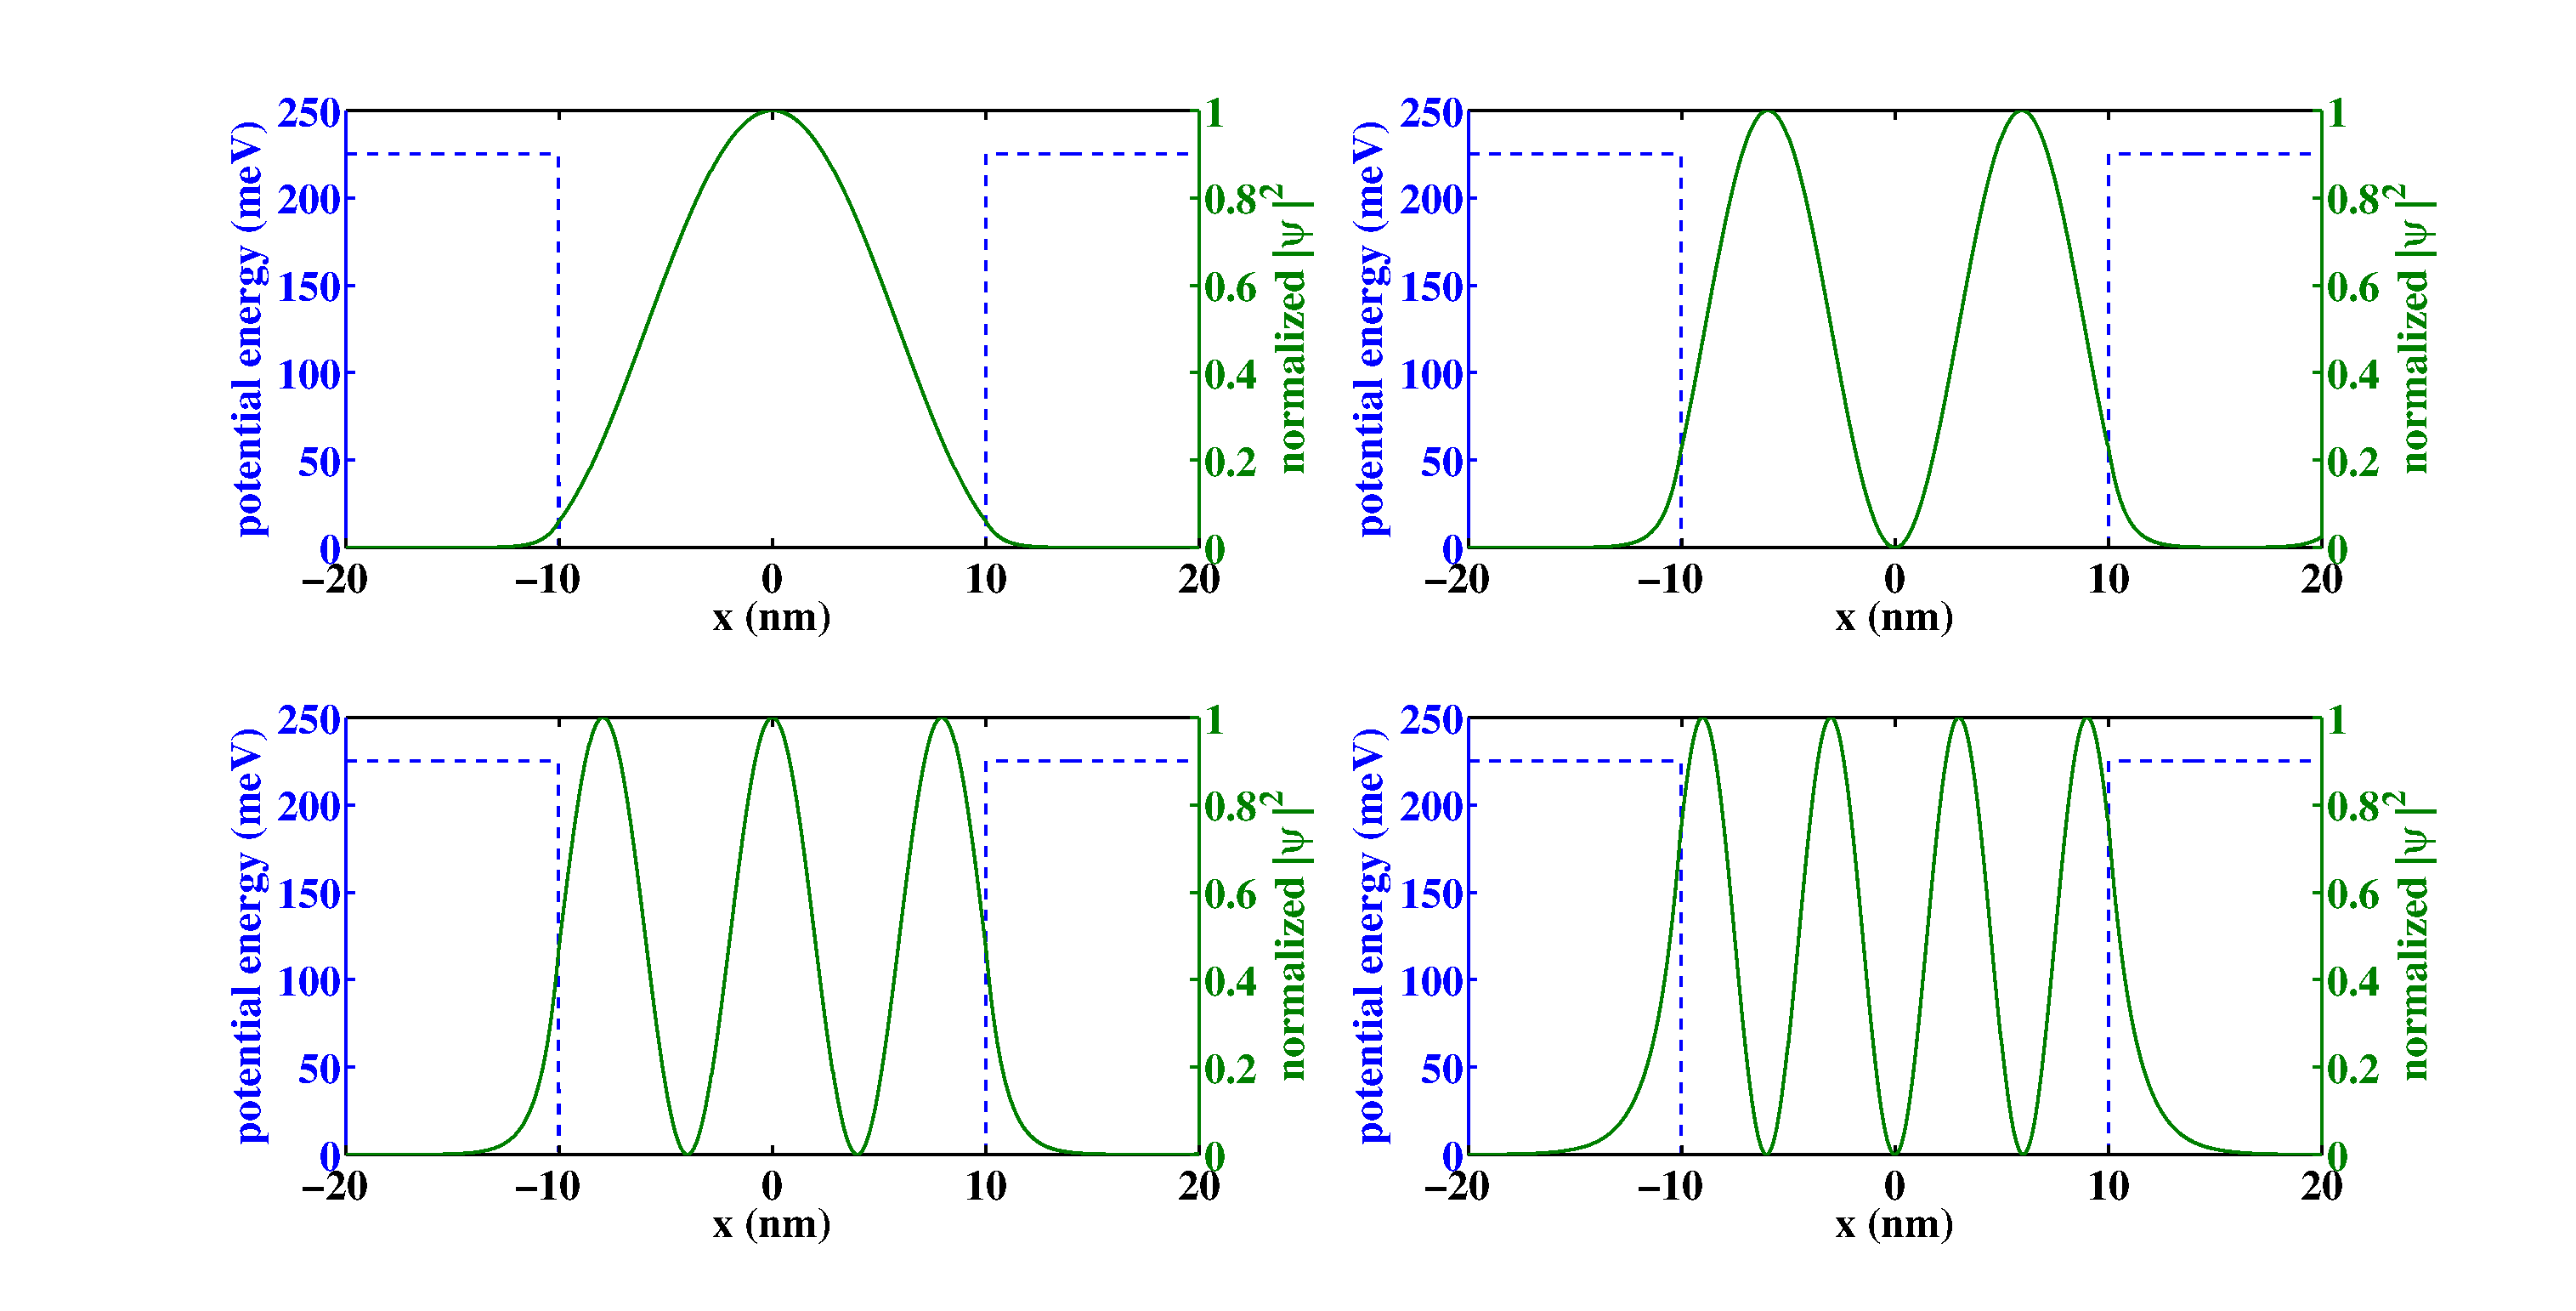
\includegraphics[width=1.0\textwidth]{./Pictures/waves.eps}\\
  \caption{势函数以及前四个能级波函数振幅的平方}
  \label{fig_waves}
\end{figure}

%%%%%%%%%%%%%%%%%%%%
\section{III-V量子阱的能带结构}
%%%%%%%%%%%%%%%%%%%%

\begin{figure}[!h]
  \centering
  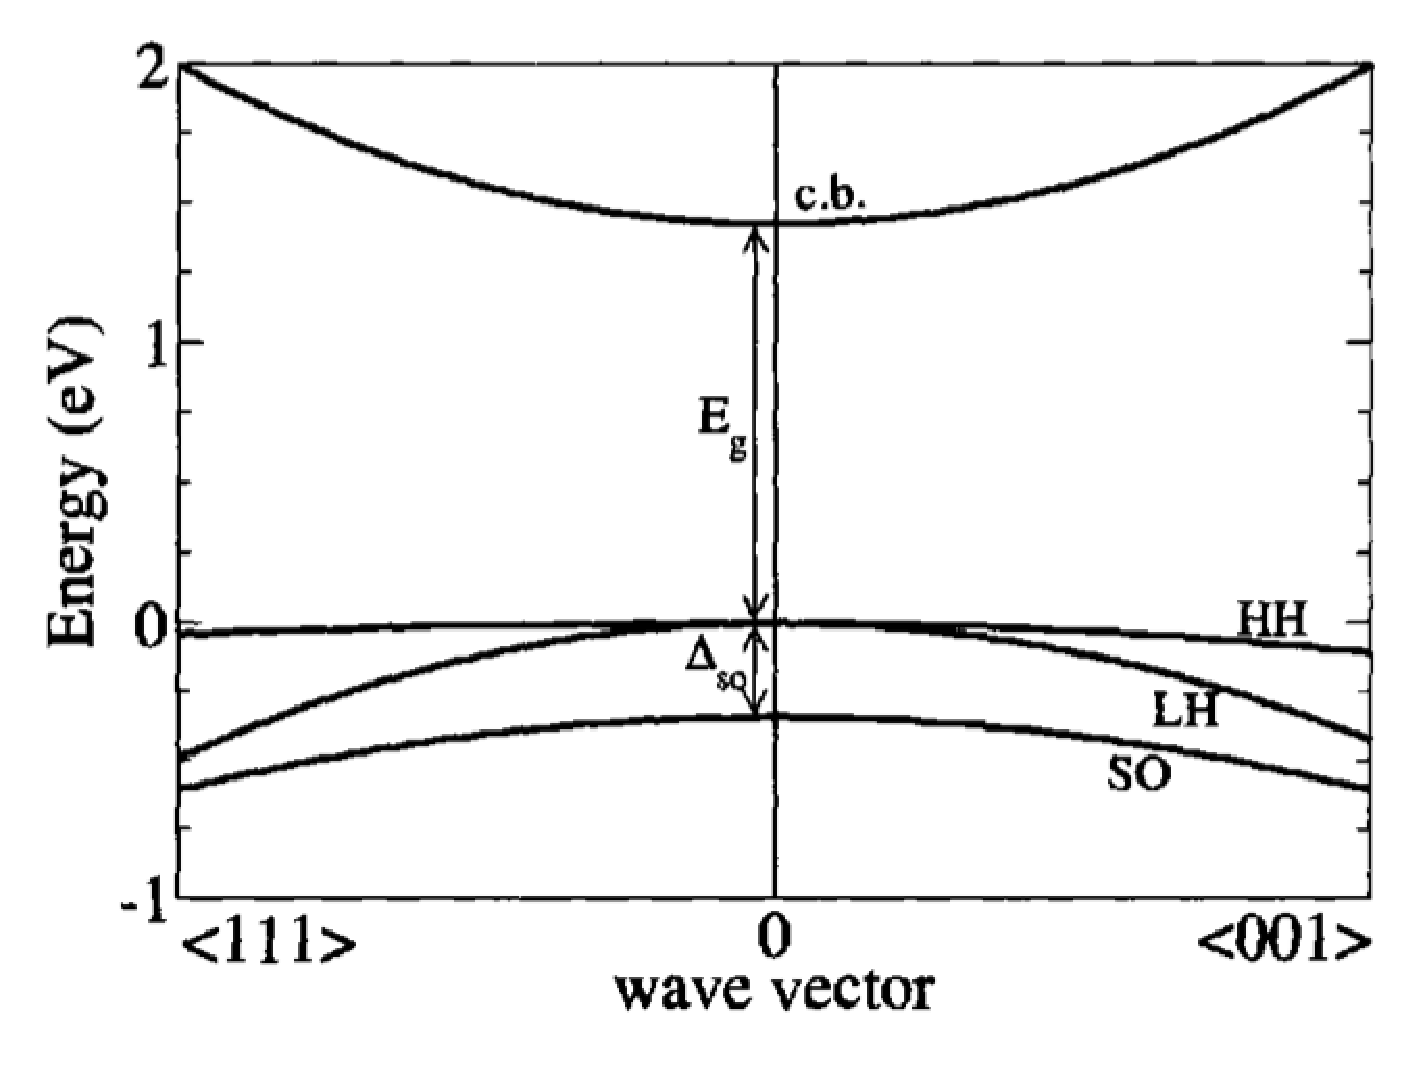
\includegraphics[width=0.7\textwidth]{./Pictures/bands.eps}\\
  \caption{III-V半导体在布里渊区的$\Gamma$点附近的导带和价带示意图}
  \label{fig_bands}
\end{figure}

对于III-V量子阱材料来说,价带的能带结构比导带要复杂一些,如图\ref{fig_bands}。通常,在布里渊区的中心附近,存在两个重叠的价带,以及在不远处的第三条能带。前面两条能带分别叫做重空穴(HH)和轻空穴(LH)带。随着波矢向远离$\Gamma$点方向运动时,重空穴带比轻空穴带向下弯曲的更慢一些,也就是对应了更大的有效质量,所以它被成为重空穴带。第三条能带叫做自旋分裂(SO)能带。也就是说,III-V材料通常包含三条价带和一条导带。为了计算这些能带,最常用也是最简单的方法是采用$k\cdot p$微扰理论,推导出计算这些能带的哈密顿算子。1955年,Luttinger和Kohn得到了关于三个价带的$6\times6$哈密顿算子,以及其中两个价带(HH和LH)的$4\times4$哈密顿算子\cite{Luttinger1955Motion}。1966年Pidgeon和Brown提出了包含导带的$8\times8$哈密顿算子\cite{Pidgeon1966Interband}。这里,我们给出Luttinger和Kohn的$6\times6$哈密顿算子如下:

\begin{equation}
    \label{eq_6times6}
    H = \left[\begin{array}{cccccc}P+Q & 0 & -S & R & (1/\sqrt{2})S & \sqrt{2}R \\0 & P+Q & -R\dag & -S^\dag & -\sqrt{2}R^\dag & (1/\sqrt{2})S^\dag \\-S^\dag & -R & P-Q & 0 & \sqrt{2}Q & \sqrt{3/2}S \\R^\dag & -S & 0 & P-Q & \sqrt{3/2}S^\dag & \sqrt{2}Q \\(1/\sqrt{2})S^\dag & -\sqrt{2}R & \sqrt{2}Q & \sqrt{3/2}S & P+\Delta_{SO} & 0 \\\sqrt{2}R^\dag & (1/\sqrt{2})S & \sqrt{3/2}S\dag & \sqrt{2}Q & 0 & P+\Delta_{SO}\end{array}\right]
\end{equation}
其中

\begin{equation}
    P = \left( \frac{h^2}{2m_0} \right) \gamma_1 (k^2_x + k^2_y + k^2_z)
\end{equation}
\begin{equation}
    Q = \left( \frac{h^2}{2m_0} \right) \gamma_2 (k^2_x + k^2_y - 2k^2_z)
\end{equation}
\begin{equation}
    R = \left( \frac{h^2}{2m_0} \right) \sqrt{3} [-\gamma_2 (k^2_x - k^2_y) + 2i \gamma_3 k_x k_y]
\end{equation}
\begin{equation}
    S = \left( \frac{h^2}{2m_0} \right) 2 \sqrt{3} \gamma_3 k_z (k_x - ik_y)
\end{equation}
其中$\gamma_{1,2,3}$是Luttinger参数,$\Delta_{SO}$是自旋轨道分裂能量。其中的参数很容易在各种书籍或文章中查到,这里不再赘述。根据以上方程,我们就可以计算出三条价带关于波失的关系。这里考虑一种特殊情况,在布里渊区的中心,我们可以将上面的算子进一步简化,即$k_x=k_y=k_z=0$时,算子变成了

\begin{equation}
    H(k=0) = \left[\begin{array}{cccccc}0 & 0 & 0 & 0 & 0 & 0 \\0 & 0 & 0 & 0 & 0 & 0 \\0 & 0 & 0 & 0 & 0 & 0 \\0 & 0 & 0 & 0 & 0 & 0 \\0 & 0 & 0 & 0 & \Delta_{SO} & 0 \\0 & 0 & 0 & 0 & 0 & \Delta_{SO}\end{array}\right]
\end{equation}
上面矩阵的含义是,当k=0时,导带和价带的能量E=0,并且自旋轨道分裂能量与他们的能力差为$\Delta_{SO}$。当我们计算量子阱时,正需要考虑这种情况。

此外,我们还需要考虑应变对价带的影响。应变在III-V半导体中表现为6个分量:$\epsilon_{xx}$,$\epsilon_{yy}$,$\epsilon_{zz}$,$\epsilon_{xy}$,$\epsilon_{zx}$和$\epsilon_{yz}$。他们对$6\times6$哈密顿算子的影响如下面的方程所示\cite{Calvin1992Spin}:

\begin{equation}
    P \rightarrow P + P_{\epsilon} ,  P_{\epsilon} = - a_v (\epsilon_{xx} + \epsilon_{yy} + \epsilon_{zz})
\end{equation}
\begin{equation}
    Q \rightarrow Q + Q_{\epsilon} ,  Q_{\epsilon} = - \frac{b}{2} (\epsilon_{xx} + \epsilon_{yy} -2 \epsilon_{zz})
\end{equation}
\begin{equation}
    R \rightarrow R + R_{\epsilon} ,  R_{\epsilon} = \frac{\sqrt{3}}{2} b (\epsilon_{xx} - \epsilon_{yy}) - i d \epsilon_{xy})
\end{equation}
\begin{equation}
    S \rightarrow S + S_{\epsilon} ,  S_{\epsilon} = - d (\epsilon_{zx} -i \epsilon_{yz})
\end{equation}
其中$a_v$,$b$,$d$是各个方向上的形变势能系数。在实际的应变量子阱材料中,随着材料在z方向外延的过程中发生了应变,所以各个方向的分量可以表示为

\begin{equation}
    \epsilon_{xy} = \epsilon_{yz} = \epsilon_{zx} = 0
\end{equation}
\begin{equation}
    \epsilon_{xx} = \epsilon_{yy} = \frac{a_0 - a_{latt}}{a_{latt}} / a_{latt}
\end{equation}
\begin{equation}
    \epsilon_{zz} = - \frac{2 C_{12}}{C_{11}}  \epsilon_{xx}
\end{equation}
其中$C_{11}$和$C_{12}$是弹性刚度系数,$a_0$是基底的晶格常数(通常都是晶格匹配的)。此时,我们再回过头来看$6\times6$哈密顿算子在k=0时的情况,他已经变成

\begin{equation}
    H = \left[\begin{array}{cccccc}P_{\epsilon}+Q_{\epsilon} & 0 & 0 & 0 & 0 & 0 \\0 & P_{\epsilon}+Q_{\epsilon} & 0 & 0 & 0 & 0 \\0 & 0 & P_{\epsilon}-Q_{\epsilon} & 0 & \sqrt{2}Q_{\epsilon} & 0 \\0 & 0 & 0 & P_{\epsilon}-Q_{\epsilon} & 0 & \sqrt{2}Q_{\epsilon} \\0 & 0 & \sqrt{2}Q_{\epsilon} & 0 & Q_{\epsilon}+\Delta_{SO} & 0 \\0 & 0 & 0 & \sqrt{2}Q_{\epsilon} & 0 & \Delta_{SO}\end{array}\right]
\end{equation}
这个方程比没有应变的情况要复杂的多。经过计算,我们可以得到k=0时三个价带在布里渊区中心的能量分别为

\begin{equation}
    E_{HH}(0) = P_{\epsilon} + Q_{\epsilon}
\end{equation}
\begin{equation}
    E_{LH}(0) = P_{\epsilon} - \frac{1}{2} \left( Q_{\epsilon} - \Delta_{SO} + \sqrt{\Delta^2_{SO} + 2 \Delta^2_{SO} Q_{\epsilon} + 9 Q^2_{\epsilon}} \right)
\end{equation}
\begin{equation}
    E_{SO}(0) = P_{\epsilon} - \frac{1}{2} \left( Q_{\epsilon} - \Delta_{SO} - \sqrt{\Delta^2_{SO} + 2 \Delta^2_{SO} Q_{\epsilon} + 9 Q^2_{\epsilon}} \right)
\end{equation}

最后,我们考虑导带和价带的偏置比,就可以得打导带和价带的势能函数方程

\begin{equation}
    \label{V_c}
    V_c(z) = Q_c E_g(z) - (1-Q_c)S_\perp(z)
\end{equation}
\begin{equation}
    \label{V_HH}
    V_{HH}(z) = (1-Q_c)[E_g(z) - S_\perp(z)] + S_\parallel(z)
\end{equation}
\begin{eqnarray}
    \label{V_LH}
    V_{LH}(z)&=& (1-Q_c)[E_g(z) - S_\perp(z)] \notag\\
    && +0.5[S_\parallel(z) + \Delta_0(z)] \notag\\
    && -0.5 \sqrt{9S_\parallel^2(z)-2S_\parallel^2(z)\Delta_0(z)+\Delta_0^2(z)}
\end{eqnarray}
其中
\begin{equation}
    \label{S_perp}
    S_\perp(z) = -2a_v(z)[1-\frac{C_{12}(z)}{C_{11}(z)}] \epsilon(z)
\end{equation}
\begin{equation}\label{S_parallel}
    S_\parallel(z) = -b(z)[1+\frac{2C_{12}(z)}{C_{11}(z)}] \epsilon(z)
\end{equation}
\begin{equation}\label{a_v}
    a_v(z) = -\frac{1}{3}[C_{11}(z)+2C_{12}(z)] \frac{dE_g}{dp}(z)
\end{equation}
\begin{equation}\label{epsilon}
    \epsilon(z) = \frac{a_{InP}(z)-a(z)}{a(z)}
\end{equation}
方程中的参数已经在表\ref{parametertable}中给出。如无特别说明,本章中采用的量子阱均采用表\ref{RedShiftSample}中的结构。


\begin{table}[!htb]
    \zihao{6}
    \caption{室温条件下(300K)InGaAsP量子阱材料的参数}
    \centering
    \label{parametertable}
    \begin{tabular}{llll}
        \hline
        \hline
        符号 & 参数 & $In_{x}Ga_{1-x}As_{y}P_{1-y}$ & 单位\\
        \hline
        $Q_c:Q_v$ & 能带偏移分裂比 & $0.6:0.4$ & $-$\\
        $E_g(z)$ & 禁带宽度 & $1.35-1.17y+0.668(1-x)-0.069y(1-x)+0.18y^2$ & eV\\
                                  && $+0.03(1-x)y^2+0.758(1-x)^2-0.322y(1-x)^2$ &\\
        $\Delta_0(z)$ & 自旋轨道分裂 & $0.34(1-x)y+0.43xy+0.10(1-x)(1-y)+0.10x(1-y)$ & eV\\
        $m_e$ & 电子质量 & $0.91095\times10{-30}$ & kg\\
        $m_c^*(z)$ & 电子有效质量 & $0.0632(1-x)y+0.0213xy+0.17(1-x)(1-y)+0.077x(1-y)$ & $m_e$\\
        $m_{\perp HH}^*(z)$ & 垂直方向 & $0.5(1-x)y+0.41xy+0.54(1-x)(1-y)+0.12x(1-y)$ & $m_e$\\
                            & 重空穴有效质量 &&\\
        $m_{\perp LH}^*(z)$ & 垂直方向& $0.088(1-x)y+0.024xy+0.16(1-x)(1-y)+0.12x(1-y)$ & $m_e$\\
                            & 轻空穴有效质量&&\\
        $m_{\parallel HH}^*(z)$ & 水平方向 & $0.11(1-x)y+0.031xy+0.19(1-x)(1-y)+0.15x(1-y)$ & $m_e$\\
                                & 重空穴有效质量 &&\\
        $m_{\parallel LH}^*(z)$ & 水平方向 & $0.23(1-x)y+0.082xy+0.34(1-x)(1-y)+0.29x(1-y)$ & $m_e$\\
                                & 轻空穴有效质量 &&\\
        $a(z)$ & 晶格常数 & $0.56533(1-x)y+0.60584xy+0.54512(1-x)(1-y)+0.58688x(1-y)$ & nm\\
        $C_{11}(z)$ & 弹性刚度常数 & $11.8(1-x)y+8.329xy+14.12(1-x)(1-y)+10.22x(1-y)$ & $10^{11}dyn/cm^2$\\
        $C_{12}(z)$ & 弹性刚度常数 & $5.38(1-x)y+4.526xy+6.253(1-x)(1-y)+5.76x(1-y)$ & $10^{11}dyn/cm^2$\\
        $dE_g/dP(z)$ & 水静压系数 & $11.5(1-x)y+10.0xy+11.0(1-x)(1-y)+8.5x(1-y)$ & $10^{-6}eV/bar$\\
        $b(z)$ & 剪切形变势能 & $-1.7(1-x)y-1.8xy-1.5(1-x)(1-y)-2.0x(1-y)$ & eV\\
        \hline
        \hline
    \end{tabular}
\end{table}


\begin{table}[!t]
    \zihao{5}
    \caption{The layer structure for the undoped InGaAsP/InP single quantum well}
    \centering
    \label{RedShiftSample}
    \begin{tabular}{cccc}
        \hline
        \hline
        No. & Composition & Thickness(nm) & Layer\\
        \hline
        5 & $In_{0.53}Ga_{0.47}As$ & 500 & Buffer/cap\\
        4 & InP & 500 & Barrier/cap\\
        3 & $In_{0.71}Ga_{0.29}As_{0.61}P_{0.39}$ & 3.5 & Well\\
        2 & InP & 300 & Barrier\\
        1 & InP & $-$ & substrate\\
        \hline
        \hline
    \end{tabular}
\end{table}

%%%%%%%%%%%%%%%%%%%%
\section{扩散模型}
%%%%%%%%%%%%%%%%%%%%

量子阱混杂的过程是一个原子扩散的过程。为了模拟这个过程,我们需要一个数学模型用来表示材料组分和扩散程度之间的关系。在这里,我们采用$A_{x}B_{1-x}C_{y}D_{1-y}$这样的标记来表示III-V族半导体化合物,其中A和B代表第III族的原子,C和D代表第V族原子,x和y分别代表相应元素的摩尔比。量子阱混杂之后,第III族和第V族的原子摩尔比可以表示为两个与晶体生长方向($z$方向)相关的函数,即$w(z)$和$v(z)$。

半导体中的扩散过程可以用沿着晶体生长方向的菲克第二定律来表示,即

\begin{equation}
  \frac{\partial{C}}{\partial{t}}=D\frac{\partial^2{C}}{\partial{z^2}}
\end{equation}

其中$C$表示材料组分,$D$表示扩散系数。一般来说,扩散系数在整个量子阱中被视为常量。在这里,我们需要引入一个用来表示扩散程度的系数,即扩散长度$L_d$。扩散长度的定义为$L_d=\sqrt{Dt}$,其中$D$是扩散系数,$t$是加热过程的时间。假设一个$In_{wx}Ga_{1-wx}As_{wy}P_{1-wy}/In_{bx}Ga_{1-bx}As_{by}P_{1-by}$的单量子阱结构,量子阱混杂之后In和As的的组分函数可以分别表示为

\begin{eqnarray}
    w(z)&=&wx-\frac{bx-wx}{2} \times \biggr[2-\textrm{erf}\biggr(\frac{L_z+2z}{4L_d^{III}}\biggr) -\textrm{erf}\biggr(\frac{L_z-2z}{4L_d^{III}}\biggr)\biggr]
\end{eqnarray}

\begin{eqnarray}
    v(z)&=&wy-\frac{by-wy}{2} \times \biggr[2-\textrm{erf}\biggr(\frac{L_z+2z}{4L_d^{V}}\biggr) -\textrm{erf}\biggr(\frac{L_z-2z}{4L_d^{V}}\biggr)\biggr]
\end{eqnarray}

在这种情况下,扩散可以同时在第III族和第V族的元素中进行,分别对应了$L_d^{III}$和$L_d^V$两个扩散长度。他们的比值$k=L_d^V/L_d^{III}$是一个影响量子阱混杂效果的重要因素。同理,对于$Al_{wx}Ga_{1-wx}As/Al_{bx}Ga_{1-bx}As$量子阱来说,由于不存在第V族元素的扩散,k值永远等于0。

\begin{figure}[!t]
    \centering
    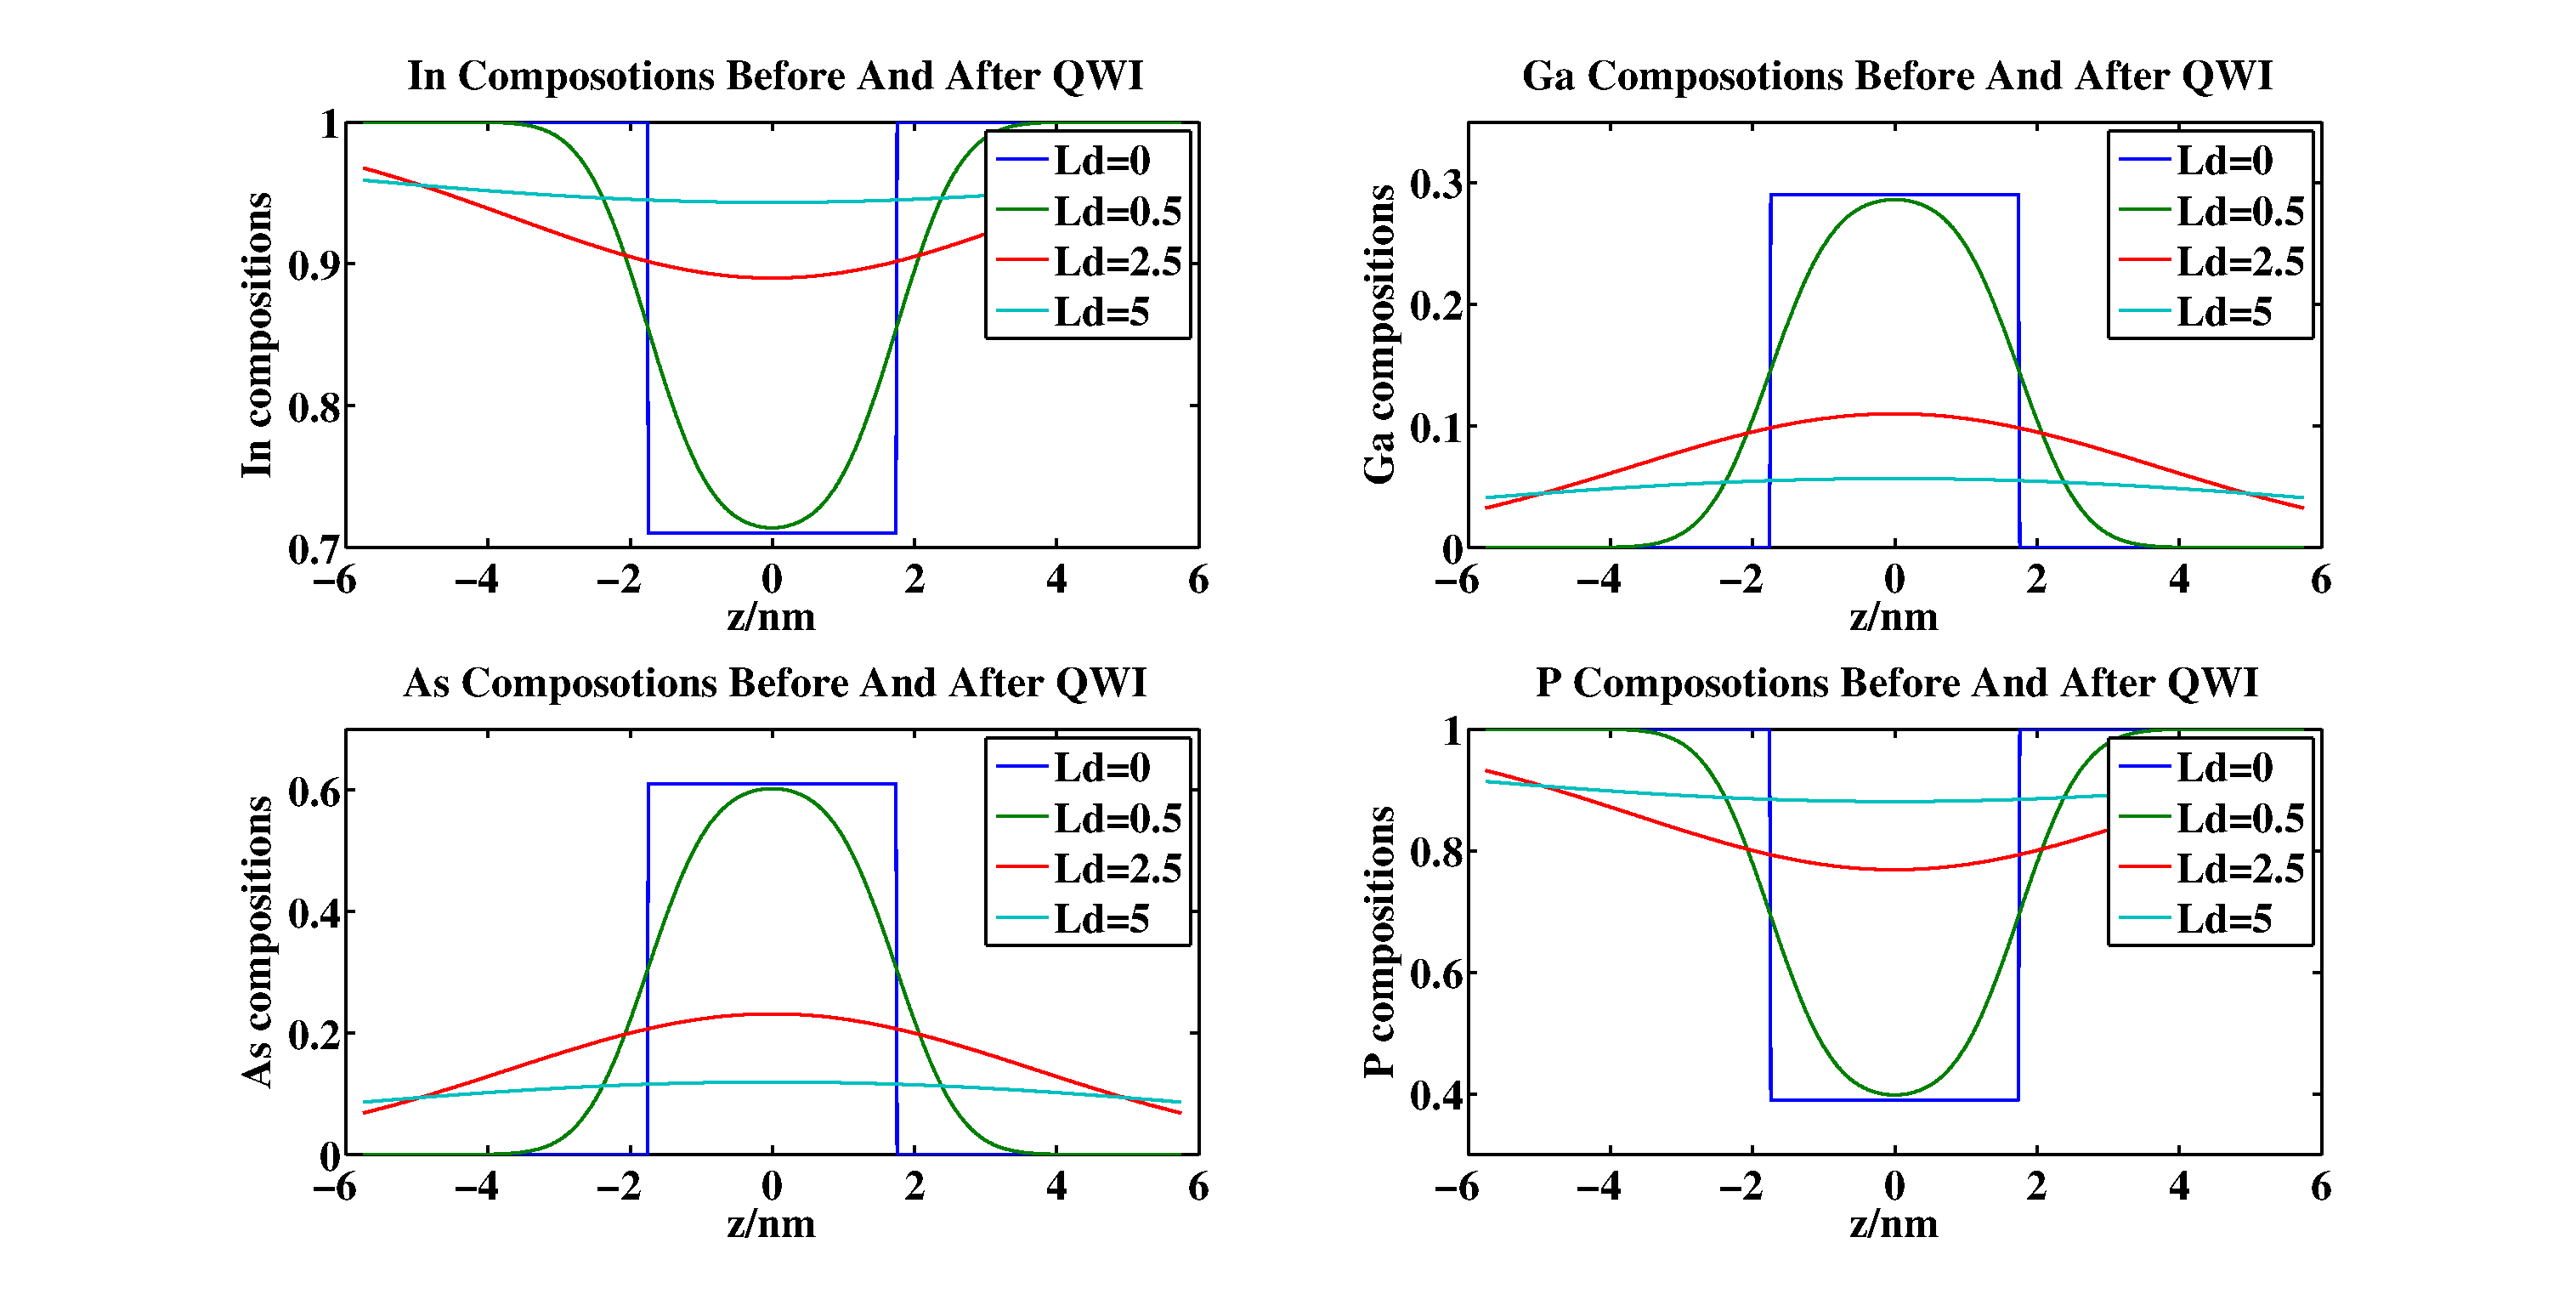
\includegraphics[width=1.0\textwidth]{./Pictures/composition.eps}
    \caption{In、Ga、As、P元素在不同的扩散长度条件下的组分分布}
    \label{fig_composition}
\end{figure}

图\ref{fig_composition}表示In、Ga、As、P元素在不同的扩散长度条件下的组分分布。当扩散长度为0时,量子阱不发生扩散,也就是不发生混杂的元素组分分布。当扩散长度为0.5nm时,元素组分仅在阱的中间位置与扩散之前的相同。当扩散长度为2.5nm时,整个阱的组分都已经发生很大变化。当扩散长度为5nm时,阱和垒的组分基本没有区别,呈现一条水平线。

%%%%%%%%%%%%%%%%%%%%
\section{扩散长度对能带结构的影响}
%%%%%%%%%%%%%%%%%%%%

为了讨论扩散长度对量子阱混杂的影响,我们假设扩散的k值始终等于1,这样就排除了k值的干扰,而且III族和V族的元素具有相同的扩散长度。我们选择了扩散长度从0到1nm,间隔0.1nm的11种情况,分别计算了导带和两条价带的最低能级的能量,如图\ref{fig_Ld_1}所示。左边的图表示In的组分变化,其实也可以看成体材料的势函数沿着材料生长方向的分布。显然,随着扩散长度的增加,量子阱的势函数的底部在不断往上抬升,这导致了导带、重空穴带和轻空穴带能级的上升,这一点从右边的图就可以清楚的看出来。

\begin{figure}[!t]
    \centering
    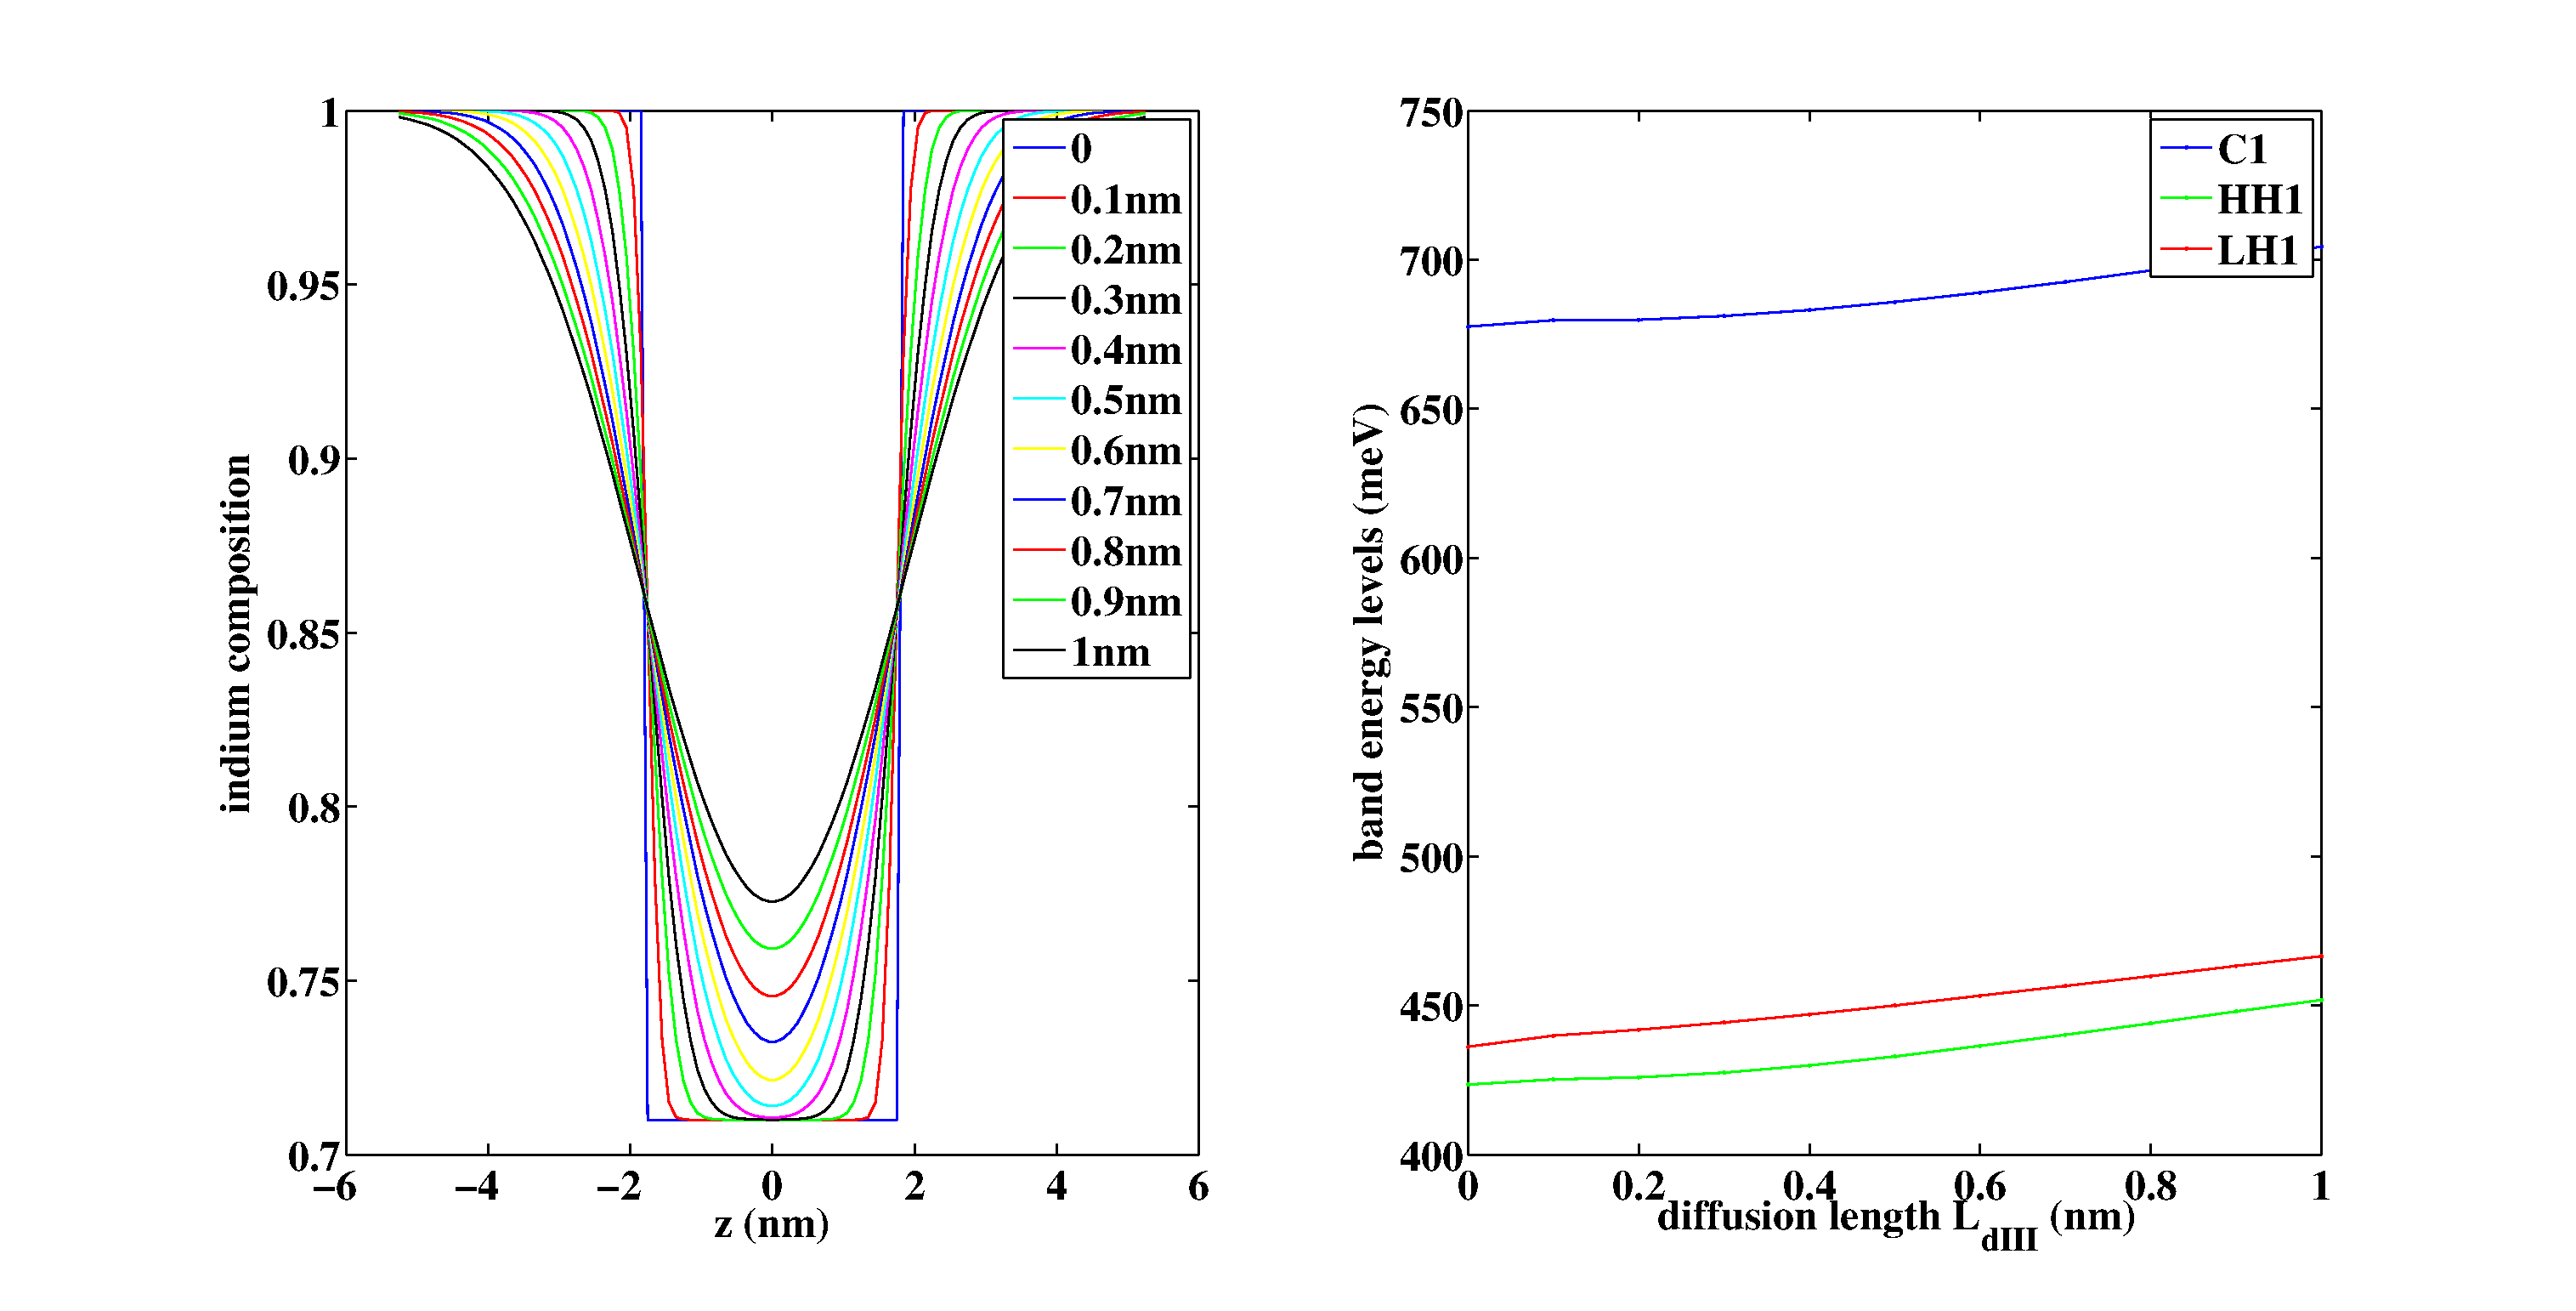
\includegraphics[width=1.0\textwidth]{./Pictures/Ld_1.eps}
    \caption{InP量子阱在不同扩散长度的条件下,导带和价带的能量变化}
    \label{fig_Ld_1}
\end{figure}

在这里,我们还可以试图将势函数的底部的能量去掉,这样一来,所有的势函数都将拥有同样的底部能量,如图\ref{fig_Ld_2}所示。这一次计算得到的能带的能量变化与之前的完全不同。从右边的图可以看到,在扩散长度小于0.5nm的时候,所有能带的能量随着扩散长度的增加而增加,这个趋势和前面是相同的。这里势函数的底部能量并没有发生变化,引起能级上升的主要因素是阱宽的变化。随着扩散长度的增加,量子阱的等效阱宽在不断减小,从而导致了量子阱能级的升高。在扩散长度大于0.5nm的时候,由于垒的势能急剧下降,导致了所有能级的能量也随之减小了。

\begin{figure}[!t]
    \centering
    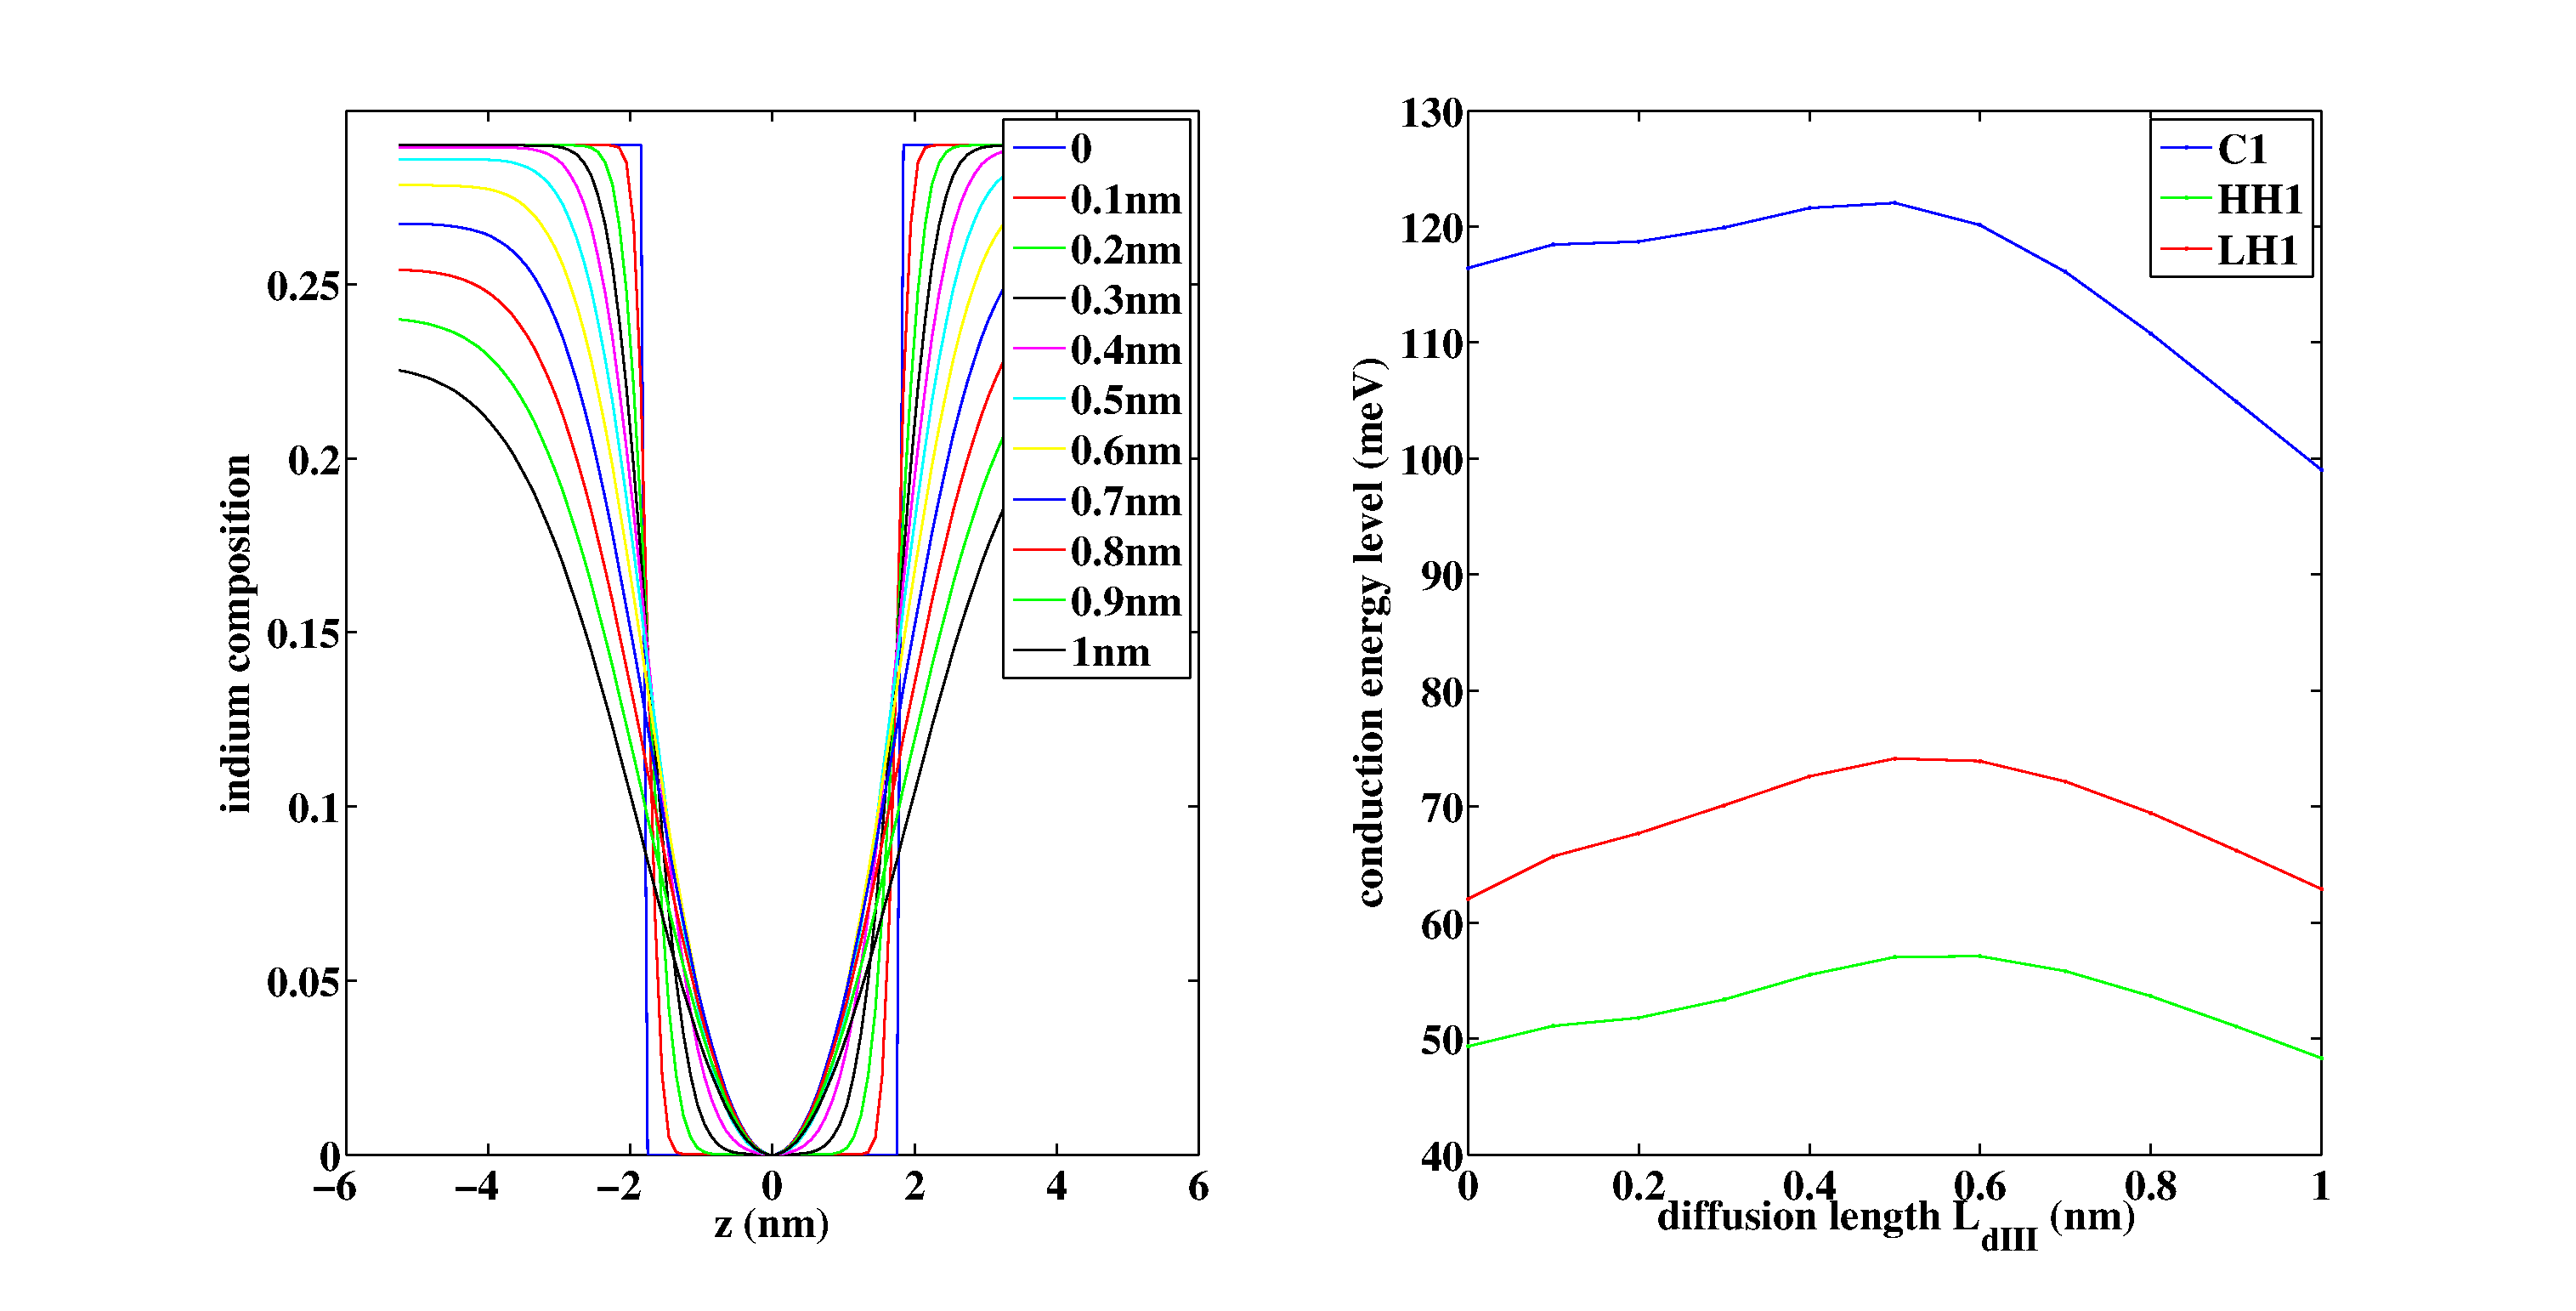
\includegraphics[width=1.0\textwidth]{./Pictures/Ld_2.eps}
    \caption{修正势函数之后的能带与扩散长度的变化关系}
    \label{fig_Ld_2}
\end{figure}

综合上述两种情况,在扩散长度比较小的情况下,阱的势能的底部还没有发生变化,这时主导能级变化的因素是等效阱宽的改变。在上面的情况中,随着扩散长度的增加,等效阱宽随之减小,这样便提升了导带和价带的能级。当扩散长度比较大时,阱的势能底部开始向上提升,垒的势能也急剧下降,他们共同导致了量子阱能级的变化。在上面的情况中,势能底的上升占据了主导地位,导致了量子阱能级随着扩散长度的增加而升高。

%%%%%%%%%%%%%%%%%%%%
\section{k值对能带结构的影响}
%%%%%%%%%%%%%%%%%%%%

除了扩散长度对蓝移会产生影响之外,k值也会影响蓝移的大小,甚至是方向。我们选择了k值为0、0.25、0.35、0.63、1的情况,分别计算C-HH和C-LH的波长变化,如图\ref{fig_k}左图所示。我们可以看到,当k=1时,对应的情况与上一节的情况完全相同,无论是C-HH还是C-LH的波长都一直往短波方向移动。当扩散长度达到10nm时,蓝移可以达到200nm以上。然而,随着k值的减小,最后能达到的蓝移也在随时减小。对于0.35和0.63两条曲线,在扩散长度大约小于2nm的时候,波长随着扩散长度的增加而增加。之后开始向短波方向移动,并且在扩散长度小于4nm的时候,仍然比一开始的波长要长。在4nm之后,波长继续往短波方向移动,最终达到约100nm左右的蓝移。对于k=0的情况,随着扩散长度的增加,波长一直向着长波方向移动,并且在最后达到约100nm的红移。综上所述,k值越小,最后能得到的最大蓝移越小,甚至可以出现红移的现象。当k值小于一定值时,波长会出现先红移,后蓝移的现象。而k值足够小的情况下,波长会一直往红移方向移动。可见,为了在单片集成中达到尽可能大的蓝移,除了扩散长度尽可能大之外,必须尽量提高k值,即尽量加剧V族元素的扩散。如果V族元素的扩散不明显的时候,也有可能发生不蓝移,甚至红移的现象。

\begin{figure}[!t]
    \centering
    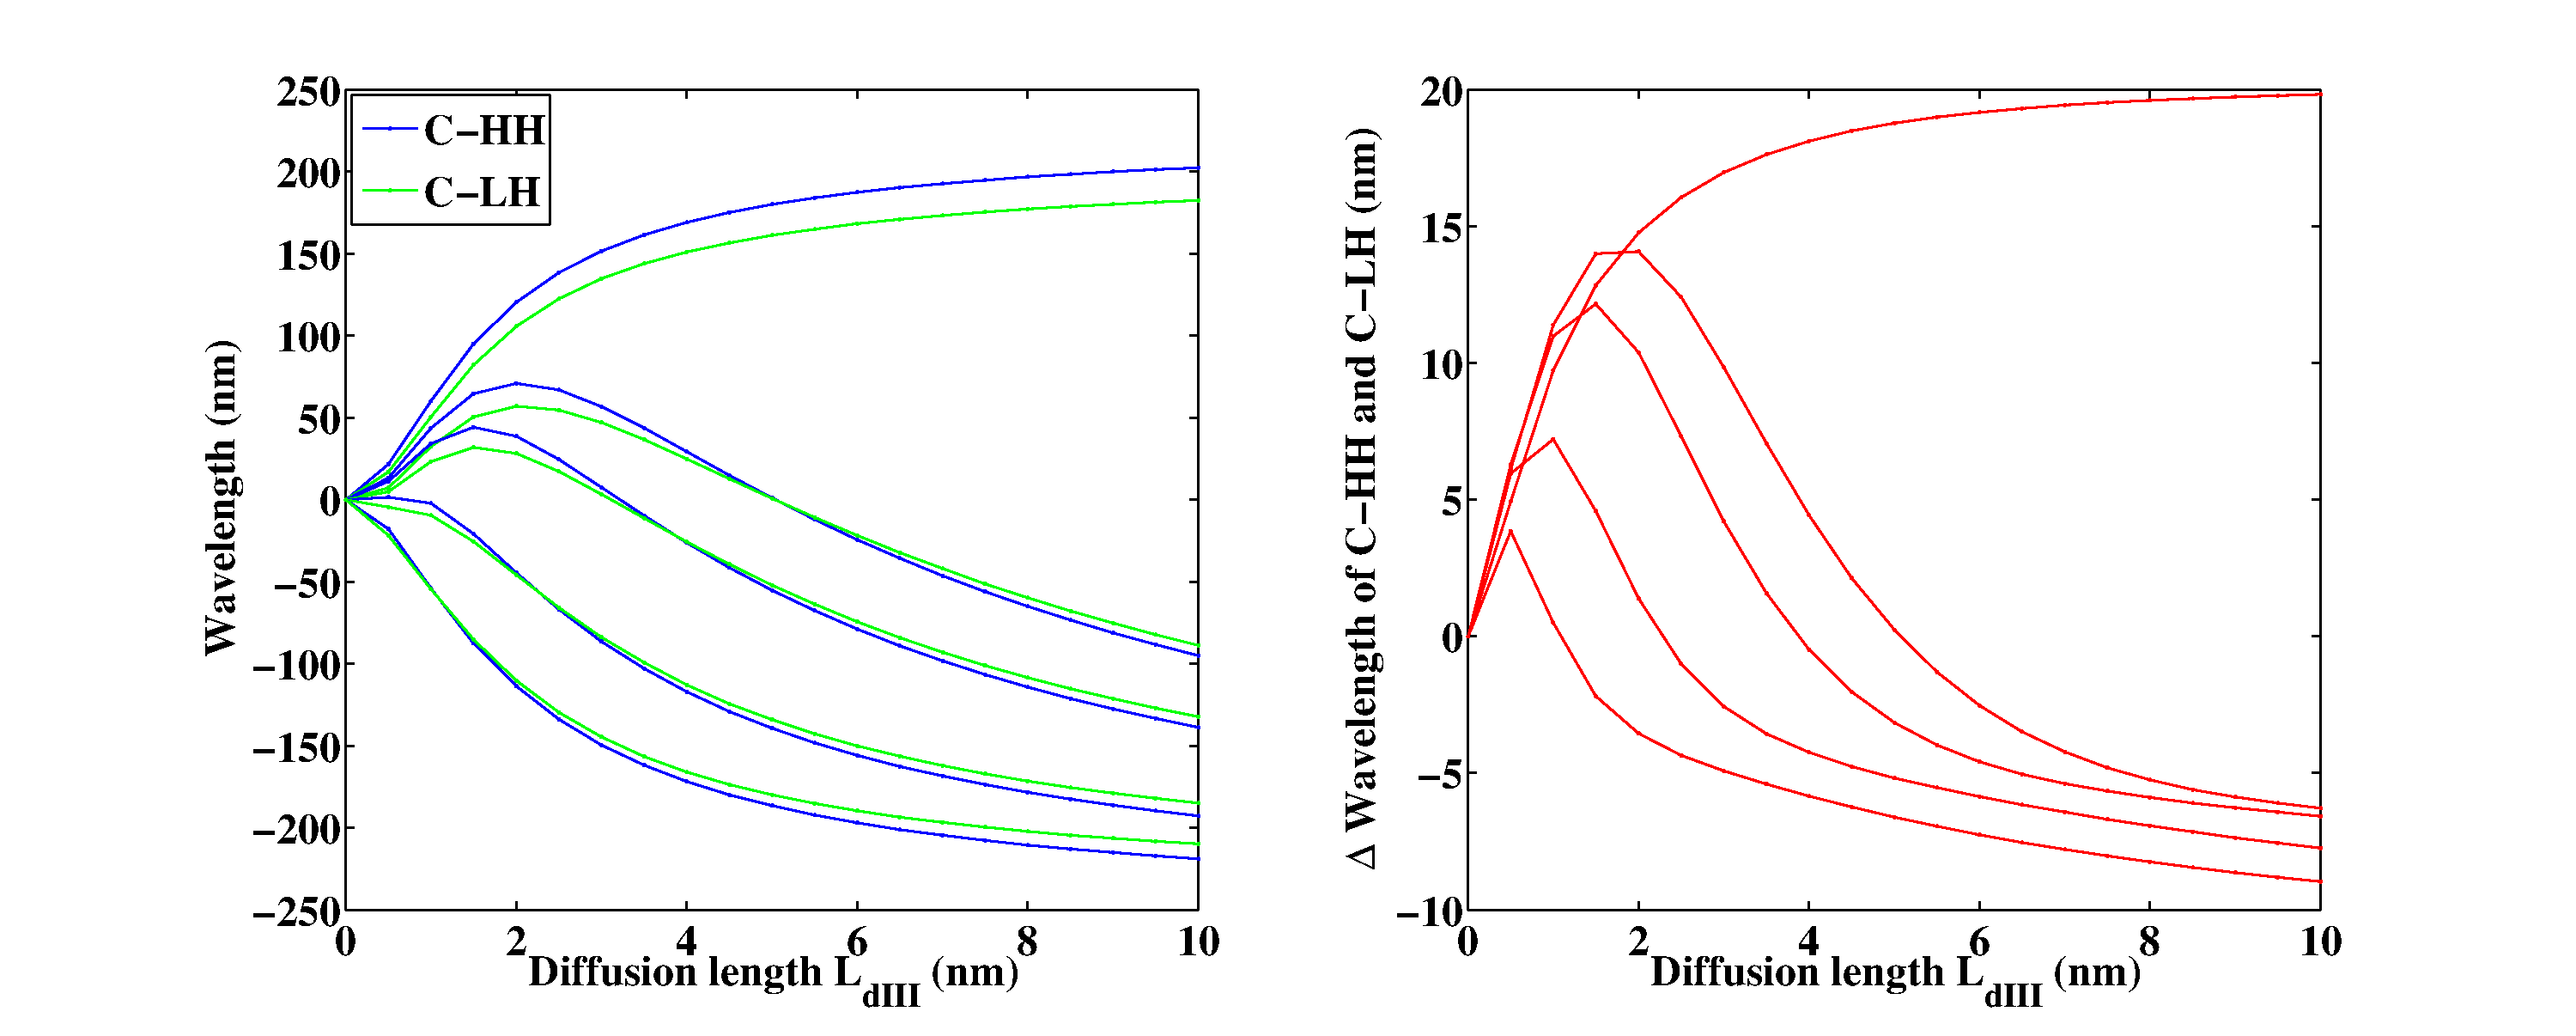
\includegraphics[width=1.0\textwidth]{./Pictures/k.eps}
    \caption{InGaAsP量子阱的C-HH和C-LH波长在不同k值和扩散长度$L_d$条件下的变化量。k值从上到下分别为0, 0.25, 0.35, 0.63, 1。}
    \label{fig_k}
\end{figure}

除此之外,我们还可以关注C-HH和C-LH变化量之间的差异,如图\ref{fig_k}右图所示。我们可以看到,无论k值取什么值,C-HH总是可以比C-LH发生更大的变化。对于通常我们希望发生的蓝移100nm以上情况,可以发现C-HH总是可以比C-LH蓝移更大。因为C-HH主要影响TE分量,而C-LH主要影响TM分量,所以在这种情况下,TE的蓝移总是比TM大。这个结论可以用来解释量子阱混杂制作的光放大器的偏振不敏感特性。1996年,J.-J. He等人提出了在InP量子阱材料上,用量子阱混杂方法制作的光放大器可以消除偏振敏感特性\cite{He1996Polarization},如图\ref{fig_amplifier}所示。在蓝移之前,TE的增益曲线对应的波长要比TM的波长大10nm左右,而在蓝移之后,两条曲线发生了重合。这说明在蓝移的过程中,TE分量比TM分量多蓝移了10nm左右,这与前面的描述是吻合的。

\begin{figure}[!t]
    \centering
    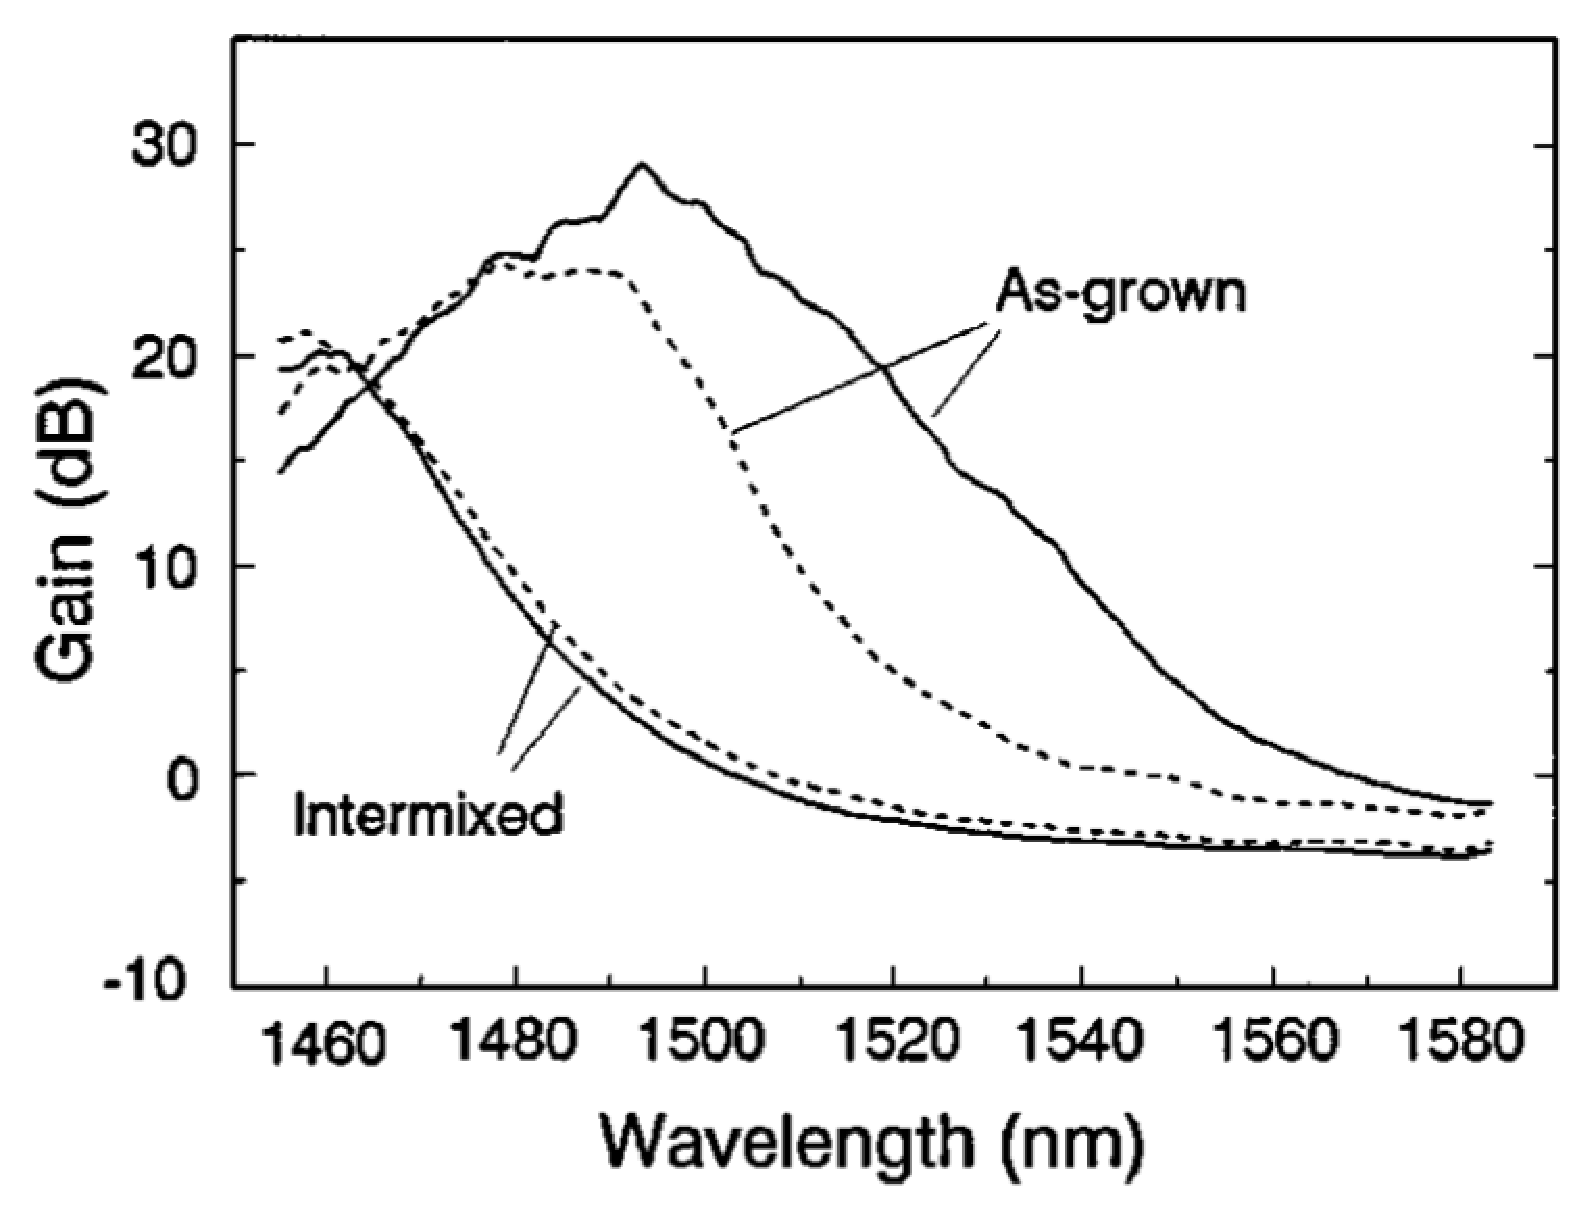
\includegraphics[width=0.7\textwidth]{./Pictures/amplifier.eps}
    \caption{测试得到的量子阱混杂之前和之后的TE和TM分量的增益曲线。其中实线表示TE分量,虚线表示TM分量。}
    \label{fig_amplifier}
\end{figure}

%%%%%%%%%%%%%%%%%%%%%%%%%%%%%%%%%%%%%%%%%%
\chapter{KrF准分子激光器照射实现量子阱混杂技术的工艺研究}
%%%%%%%%%%%%%%%%%%%%%%%%%%%%%%%%%%%%%%%%%%

待添加。

%%%%%%%%%%%%%%%%%%%%%%%%%%%%%%%%%%%%%%%%%%
\chapter{量子阱混杂技术在集成光子回路中的应用}
%%%%%%%%%%%%%%%%%%%%%%%%%%%%%%%%%%%%%%%%%%

%%%%%%%%%%%%%%%%%%%%
\section{V型腔激光器}
%%%%%%%%%%%%%%%%%%%%

随着密集波分复用(DWDM)技术的广泛使用,波长敏捷型光子集成回路变得越来越重要。波分复用技术通过在一路光纤中传输多路光信号的方法,增加了网络的带宽。国际通信联盟(ICU)制定了WDM的基本规则。现在的光信道的间隔为100GHz或0.8纳米,未来将会变成50GHz或25GHz。要实现WDM,就需要激光器覆盖ICU规定的每个信道。想要覆盖这么多的信道,使用大范围可调谐激光器是一个明智的选择。

现在人们在实验室已经制造出了很多种大范围可调谐激光器。其中一种就是V型腔激光器。V型腔激光器的示意图如图\ref{fig_vccl}所示。其主要部分包含两个长度不同的光学谐振腔,一个耦合相位为 180°的半波耦合器以及一个波长调谐区。另外在V字型的闭合端(图\ref{fig_vccl}中右端)有一个耦合器,V字型的开口端(图\ref{fig_vccl} 中左端)为一个多模耦合器(MMI)。

\begin{figure}[!h]
  \centering
  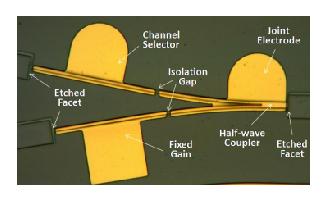
\includegraphics[width=0.7\textwidth]{./Pictures/vccl.eps}\\
  \caption{V型腔激光器的光学显微镜图\cite{jin201116-VCCL}}
  \label{fig_vccl}
\end{figure}

其中第一个光学谐振腔由一段光波导以及两端的深刻蚀反射槽构成,该段光学波导上面镀有一段电极用来注入电流以提供激光器谐振所需的增益,我们称之为固定增益腔(Fix Gain Cavity)。第二个光学谐振腔由两段光学波导以及两端的深刻蚀反射槽构成,其中一段波导提供增益,另一段波导为无源波导,可以通过注入电流来改变其光学长度从而来调谐激光器的工作波长,因此称之为信道选择腔(Channel Selector Cavity)。两段波导中间由一个浅刻蚀槽隔开。在V字型的闭合端,两个谐振腔中间由一个耦合相位为 180°的半波耦合器相连,通过设计优化两个腔之间的耦合系数可以使得整个复合耦合腔激光器实现高的边模抑制比和良好的单模特性。另外波长调谐区离耦合区较远,使得其折射率的改
变几乎不影响两个谐振腔之间的耦合系数。左端的MMI 耦合器用来将两根波导的输出光耦合到一跟波导,同时可以通过调节一个臂的注入电流来切换光输出的端口,用以做空间光开光。

为了实现激光器工作波长的数字式调谐,固定增益腔的长度要根据激光器的工作波长来确定,使得固定增益腔的谐振频率的间隔与预先要求的频率间隔一致,例如根据ITU的规定,各个通信波长的间隔为200GHz、100GHz或者50GHz等。谐振腔的频率间隔可由下式确定:
\begin{equation}
  \Delta f = \frac{c}{2 n_g L}
\end{equation}

其中$c$是真空中的光速,$n_g$是波导的有效群折射率,$L$是固定增益腔的长度。

同样,第二个谐振腔(信道选择腔)的频率间隔$\Delta f ^\prime$由式\ref{eqa_Daltafprime}决定:
\begin{equation}\label{eqa_Daltafprime}
  \Delta f ^\prime= \frac{c}{2 n_g^\prime L^\prime} = \frac{c}{2 (n_a L_a + n_b L_b)}
\end{equation}

其中$L_a$和$L_b$分别为信道选择腔的增益区以及波长调谐区的长度,同样$n_a$和$n_b$分别为信道选择腔的增益区以及波长调谐区的有效群折射率。$L^\prime=L_a+L_b$是信道选择腔的总长度,$n_g^\prime=(n_a L_a + n_b L_b)/L^\prime$是信道选择腔的平均有效群折射率。

信道选择腔的频率间隔$\Delta f ^\prime$选择为与固定增益腔的频率间隔$\Delta f$有一个微小的差别,这使得在工作物质的增益窗口内,两者只有一个谐振峰恰好重合(如图\ref{fig_Deltaf}所示)。两个谐振腔相邻的互相重合的谐振峰之间的间隔为组合腔的自由光谱范围(FSR),其大小由式\ref{eqa_Daltafc}决定。为了避免两个波长同时被激发,$\Delta f_c$一般来讲必须大于激光器工作物质增益窗口的宽度。
\begin{equation}\label{eqa_Daltafc}
  \Delta f_c = \frac{\Delta f \Delta f^\prime}{|\Delta f-\Delta f^\prime|}
\end{equation}
\begin{figure}[!h]
  \centering
  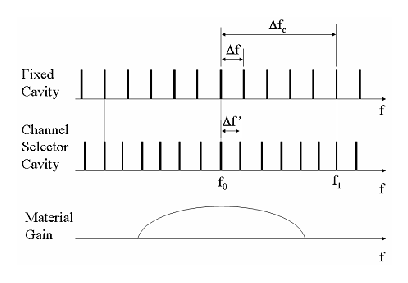
\includegraphics[width=0.7\textwidth]{./Pictures/deltaf.eps}\\
  \caption{固定增益腔和信道选择腔的谐振频率位置关系的示意图,以及激光工作物质的增益光谱曲线}
  \label{fig_Deltaf}
\end{figure}

固定增益腔以及信道选择腔的谐振频率分别为:
\begin{equation}
  f = \frac{mc}{2nL}
\end{equation}
\begin{equation}
  f^\prime = \frac{m^\prime c}{2n^\prime L^\prime}
\end{equation}
其中$m$和$m^\prime$都是整数,$n$和$n^\prime$分别为两个腔的平均有效折射率,$L$和$L^\prime$ 分别为两个腔的长度。信道选择腔的谐振频率$f^\prime$可以通过改变波长调谐区的折射率$n_b$从而改变整个腔的有效折射率$n^\prime$而改变。频率调谐量由下式决定:
\begin{equation}
  \frac{\delta f^\prime}{f^\prime} = -\frac{\delta n^\prime}{n^\prime}=-\frac{\delta n_b L_b}{n_b L^\prime}
\end{equation}

由于激光器的工作频率为固定增益腔与信道选择腔谐振峰重合的频率,因此$|\Delta f-\Delta f^\prime|$一个较小的变化将会导致激光器工作频率跳变一个信道。因此,激光器工作频率的改变量被放大了一个因子$\Delta f/|\Delta f-\Delta f^\prime|$,即:
\begin{equation}
  \delta f = \frac{\Delta f}{|\Delta f-\Delta f^\prime|} \delta f^\prime
\end{equation}

这种效应称作为游标效应。取样光栅(Sample Grating ,SG) 、超结构光栅(Super Structure Grating,SSG)也是利用类似的原理,但是取样光栅,超结构光栅的频率间隔是由光栅的调制周期决定,而且通常至少需要10个周期以上,为了获得同样的频率间隔,取样光栅超结构光栅的器件长度通常为V 型腔的20倍左右。

鉴于通常的ITU 标,假设$\Delta f=100GHz$,$\Delta f^\prime=90GHz$,则激光器工作频率的调节范围与仅靠调节折射率相比扩大了10倍。在上述数据下,设波导的有效群折射率为3.215,则固定增益腔以及信道选择腔的长度分别为:$L=466.24\mu m$,$L^\prime=518.31\mu m$,其长度与传统的DFB以及法布里- 珀罗激光器相当。相比之下,取样光栅、超结构光栅DBR激光器,由于受到器件长度以及损耗的限制,通常的信道间隔至少为600GHz,而对于通常的密集波分复用系统(DWDM)信道间隔一般为50GHz~200GHz,很难实现完全的数字式调谐。对于V型耦合腔宽带可调谐激光器,则完全不受此限制,并且利用深刻蚀槽做反射面技术,通过全息平版照相(photolithographic)技术可以精确控制激光器谐振腔的长度。激光器工作波长与ITU标准的些许偏离可以由微调固定腔的注入电流以及温度调谐来补偿。

%%%%%%%%%%%%%%%%%%%%
\section{电调谐与热调谐的区别}
%%%%%%%%%%%%%%%%%%%%

尽管V型腔激光器已经在InP和GaAs材料上同时取得了成功,但是他们距离实际商业应用还有很长的路要走。在光通信领域中,为了得到更快的速度,我们常常会使用尽可能快的调制器,例如电吸收调制器可以将调制速度提升到40Gbps(文献?),甚至使用行波电极做到100Gbps(?)。除了提升同一个波长信号的调制速度,还要提升不同波长信号之间的切换速度。2012年,浙江大学的郭山溧等人测试了V型腔激光器的波长切换速度\cite{guo2012experimental}。他们所测试的激光器波长调谐曲线如图\ref{fig_gsl_tuning}所示。在波长调谐电流大于45mA的情况下,激光器的输出波长随着电流的增加而增加,这与之前的所有文章中的结果是一致的,也就是热调谐。而当调谐电流小于20mA时,激光器的输出波长随着电流的增加而减小,这与之前的情况刚好相反,这主要是载流子注入调谐,也就是电调谐在起作用。而在20mA和45mA之间的部分,波长没有发生跳变,也就是电调谐和热调谐的作用刚好相互抵消。然后,他们选择了其中的四个波长,如表\ref{tab_4wavelength}所示。其中,通道A和通道B之间的切换时间通过光外差方法测试得到仅有500ps,也就是相当于2G的速度。而通道3和通道4之间的切换时间通过光滤波器方法测试得到有20us,也就是相当于50k的速度。显然,热调谐的速度远远小于电调谐的速度。同时,电调谐需要的电流远小于热调谐的电流,这样还可以减小整个激光器的功耗。在实际的光通信应用中,我们需要的是电调谐的V型腔激光器。

\begin{figure}[!h]
    \centering
    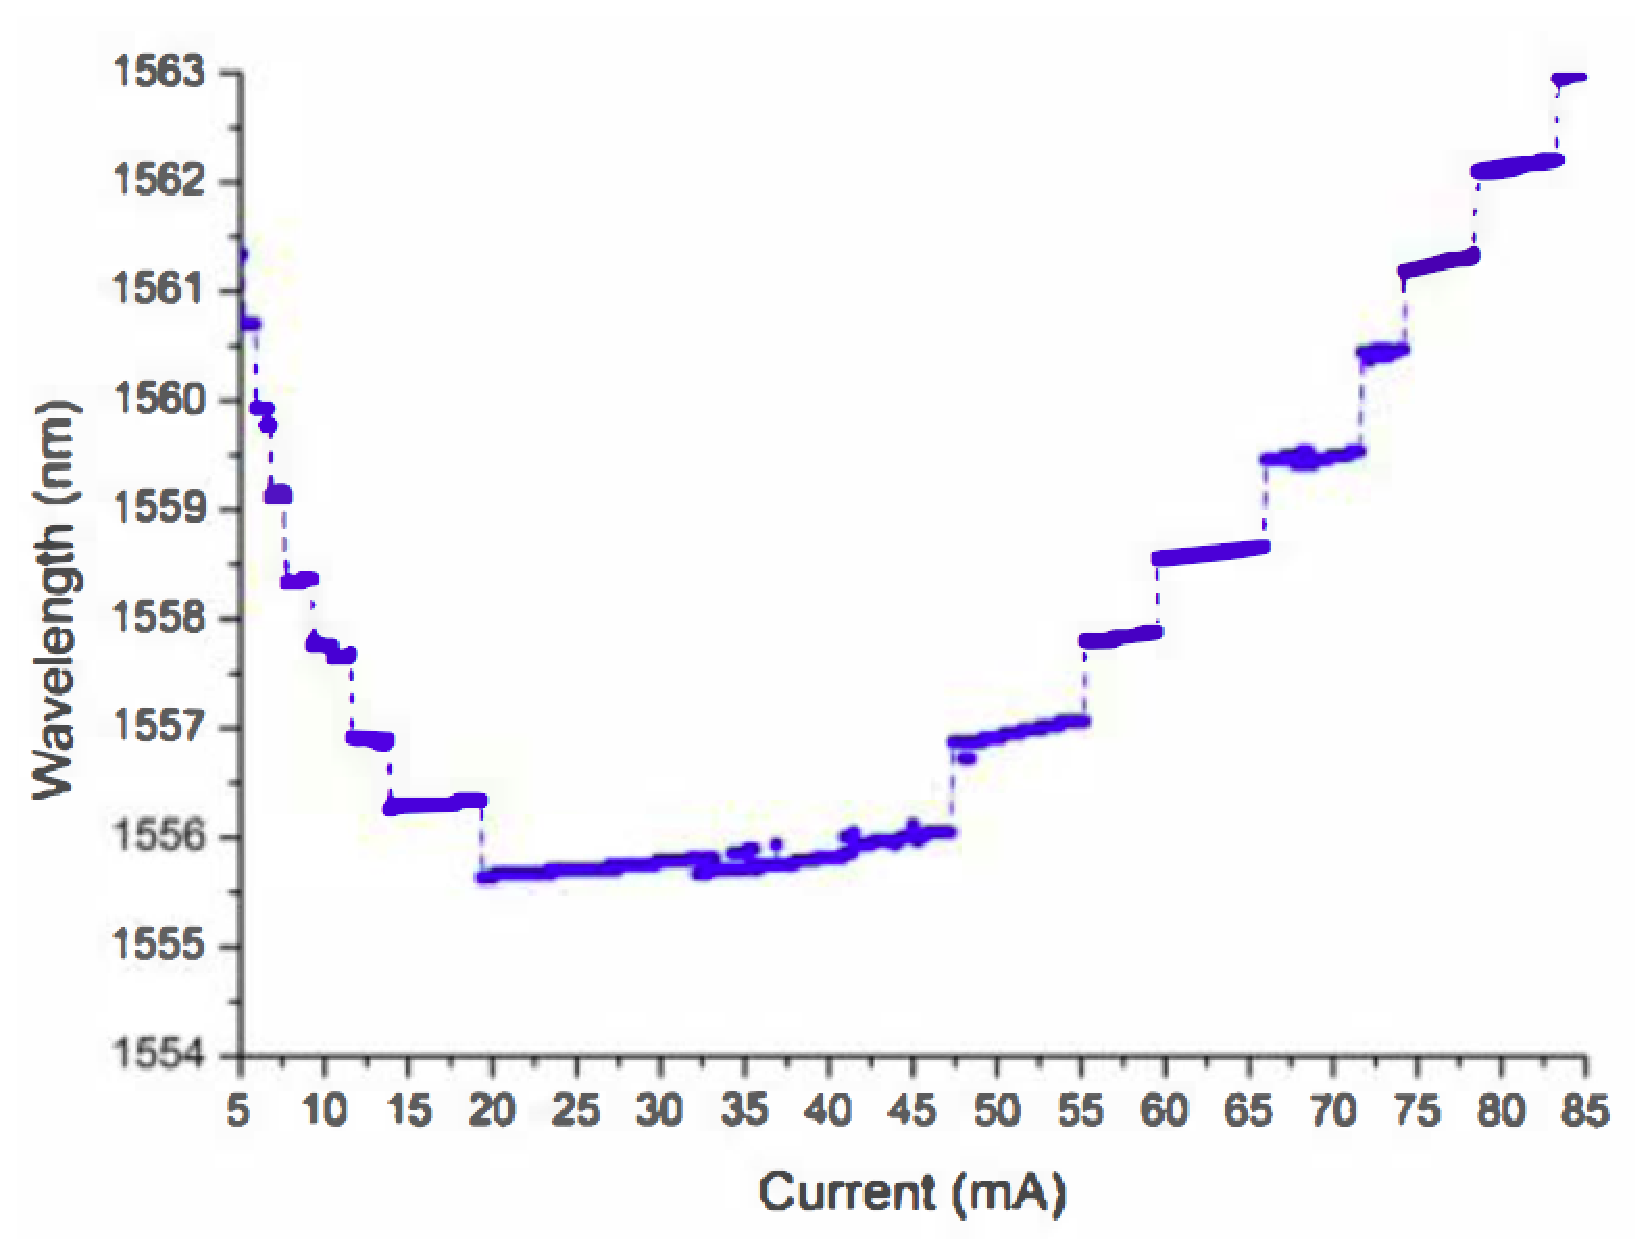
\includegraphics[width=0.7\textwidth]{./Pictures/GSL_tuning.eps}
    \caption{V型腔激光器的波长调谐曲线}
    \label{fig_gsl_tuning}
\end{figure}

\begin{table}[!t]
    \zihao{5}
    \caption{测试的4个波长以及对应的电流}
    \centering
    \label{tab_4wavelength}
    \begin{tabular}{ccccc}
        \hline
        \hline
         & 通道A & 通道B & 通道C & 通道D\\
        \hline
        电流(mA) & 17 & 25 & 	39 & 49\\
        波长(nm) & 1556.33 & 1555.70 & 1555.88 & 1556.67\\
        \hline
        \hline
    \end{tabular}
\end{table}

然而,要实现电调谐的V型腔激光器并没有那么简单。在郭山溧的文章中,我们可以看到电调谐得到的波长通道仅有8个,而且他们的边模抑制比特性甚至由于太不好而没有给出。所以,我们希望将电调谐和热调谐达到平衡的流量值,尽可能往大电流的方向上移动,同时能保持输出光谱的边模抑制比在35dB以上。其中一种方法就是将V型腔的调谐腔处理成无源腔。2003年,加州大学圣芭芭拉校区的Erik J. Skogen等人研究了量子阱混杂的蓝移对载流子注入调谐的范围影响,如图\ref{fig_qwi_tuning}所示。显然,蓝移最大的情况下能得到的载流子注入调谐的范围也是最大的。这说明了我们需要在V型腔的调谐腔上做出尽可能大的蓝移,同时不改变材料的其他特性。

\begin{figure}[!h]
    \centering
    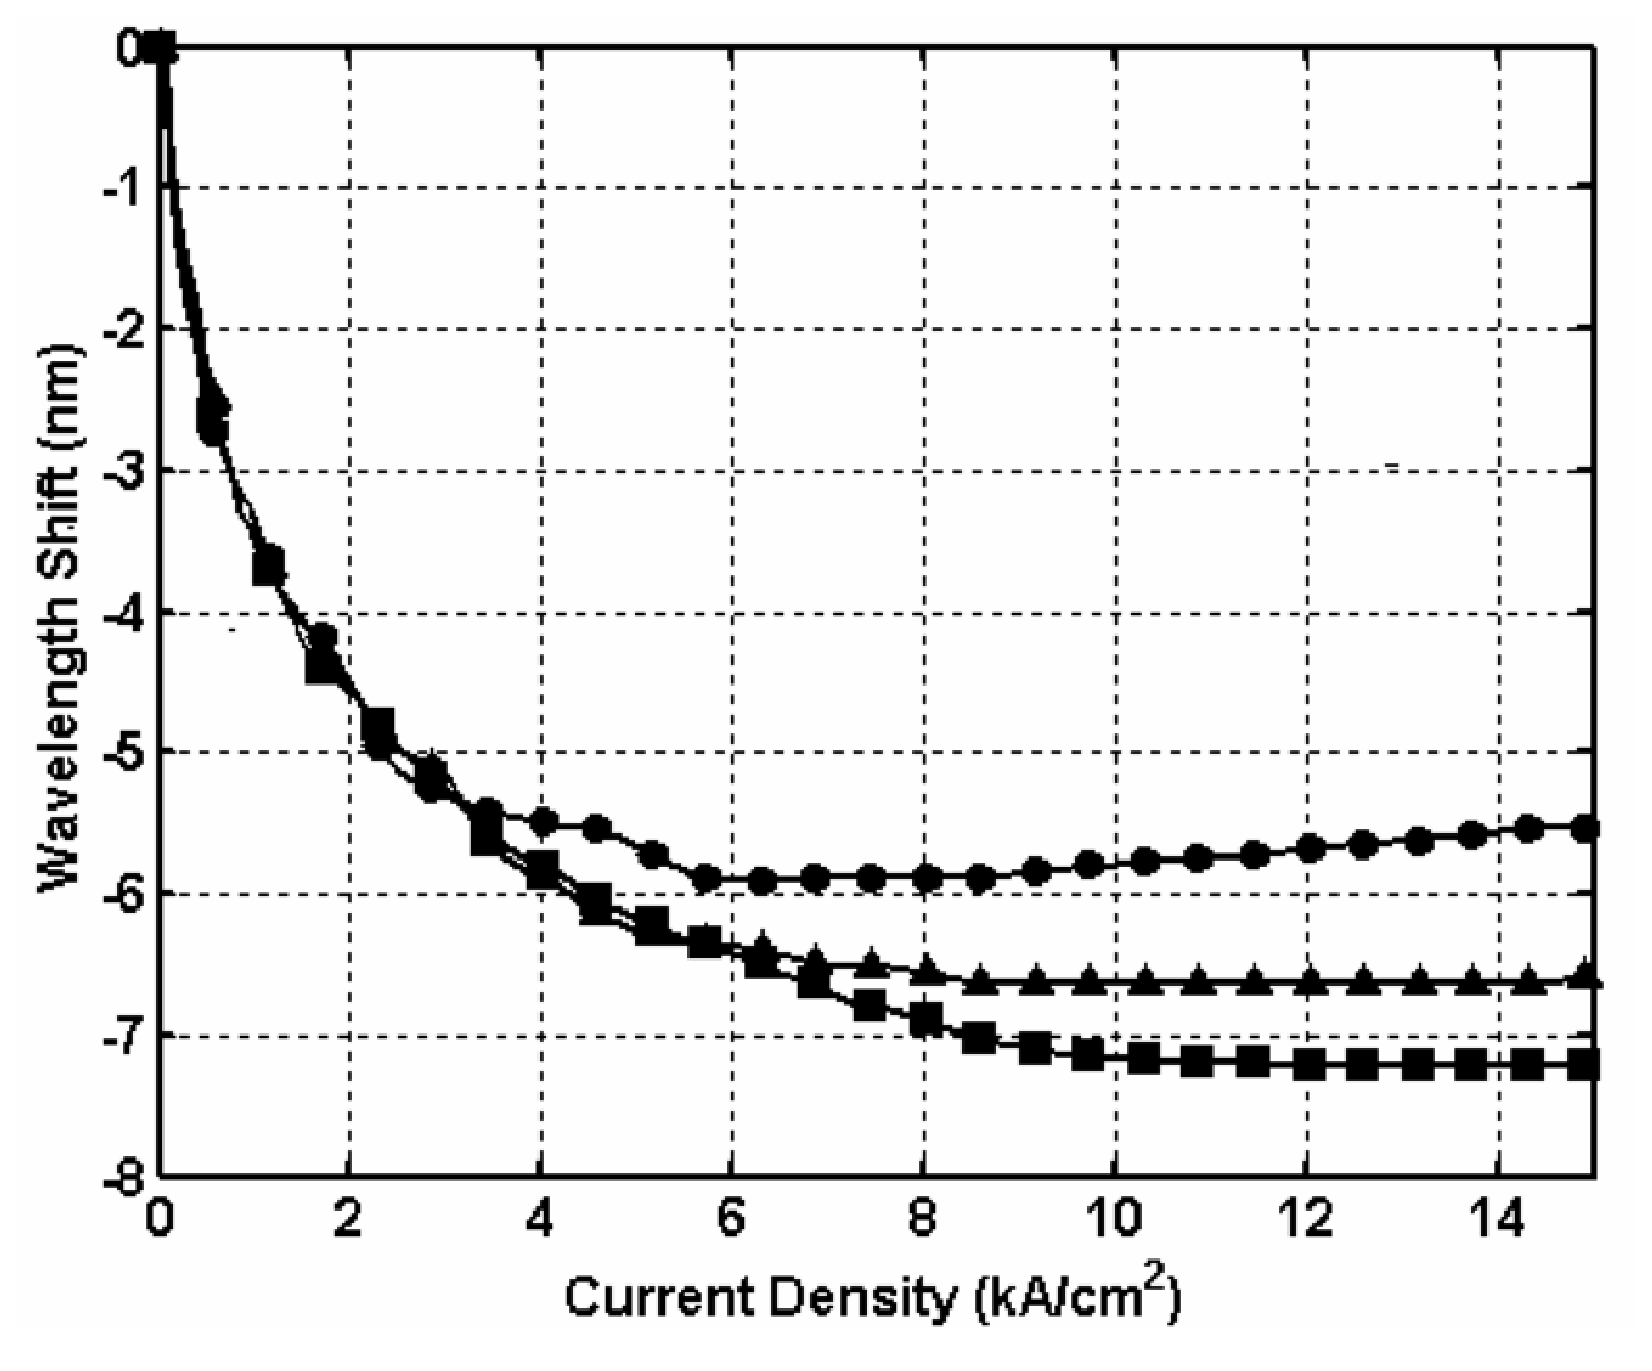
\includegraphics[width=0.7\textwidth]{./Pictures/qwi_tuning.eps}
    \caption{量子阱混杂的蓝移大小(圆形1475nm,三角形1446nm,方形1423nm)对载流子注入调谐大小的影响}
    \label{fig_qwi_tuning}
\end{figure}

%%%%%%%%%%%%%%%%%%%%
\section{包含量子阱混杂的V型腔激光器的制作过程}
%%%%%%%%%%%%%%%%%%%%

包含量子阱混杂的V型腔激光器的AutoCAD设计图如图\ref{fig_vccl_design}所示。其中红色部分为量子阱混杂掩膜,浅蓝色部分为深刻蚀面掩膜,深蓝色部分为波导掩膜,黄色部分为电极掩膜。为了区分长腔和短腔的电极,短腔的电极设计成了方形。整个制作过程可以分成以下五个部分:

\begin{enumerate}
\item{制作对准标记}
\item{利用KrF紫外激光器照射的方法在红色的掩膜内部实现量子阱混杂}
\item{制作深刻蚀面}
\item{制作波导}
\item{制作电极,减薄,退火}
\end{enumerate}


\begin{figure}[!h]
    \centering
    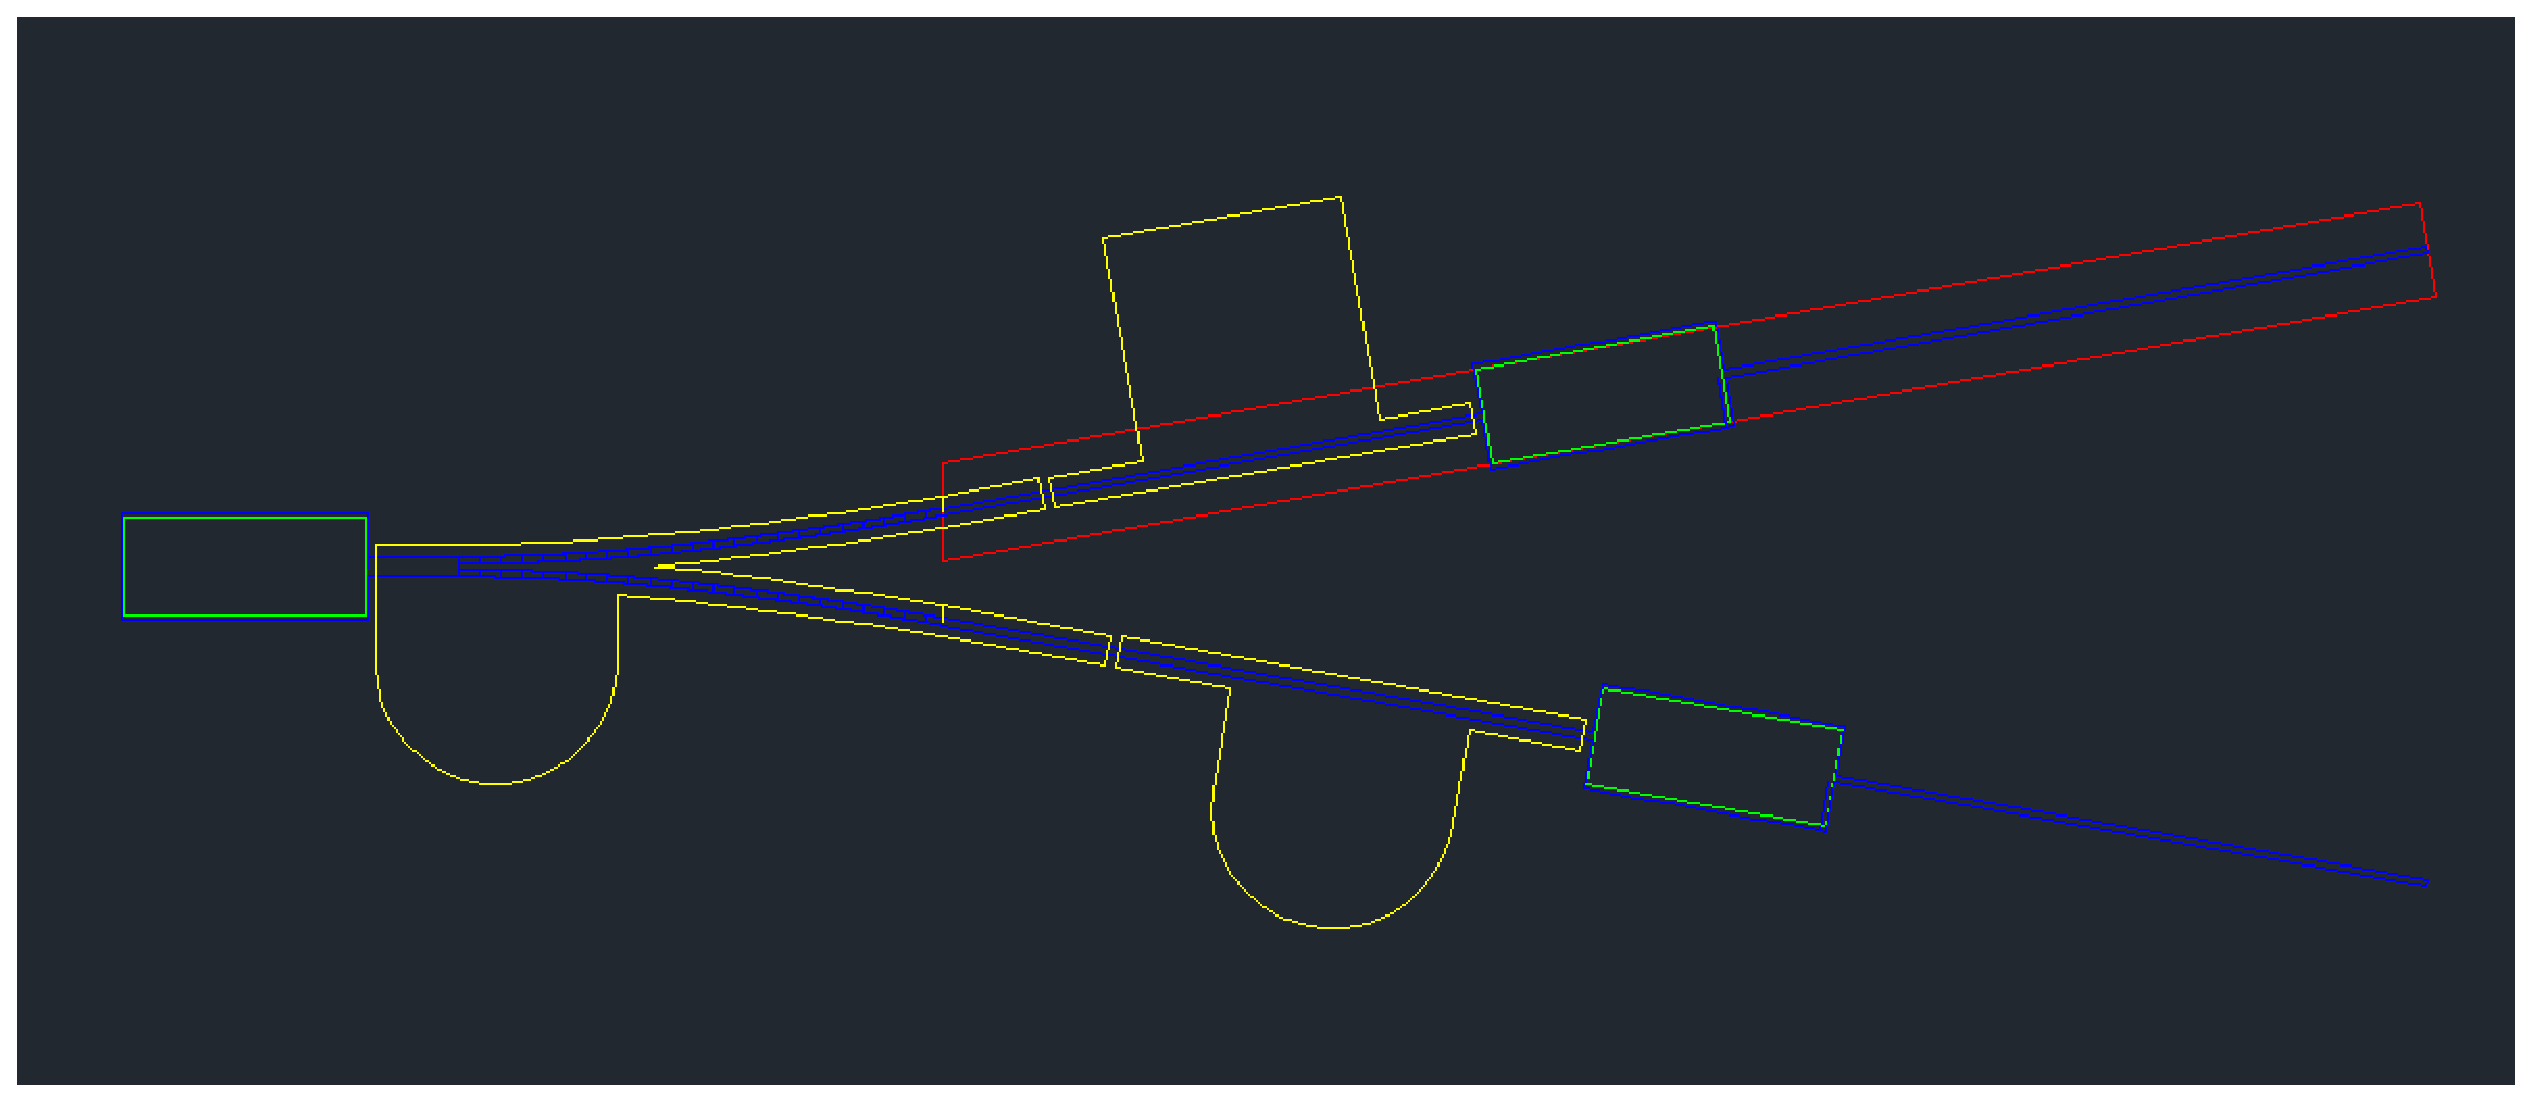
\includegraphics[width=0.7\textwidth]{./Pictures/vccl_design.eps}
    \caption{包含量子阱混杂的V型腔激光器的AutoCAD设计图}
    \label{fig_vccl_design}
\end{figure}

\subsection{制作对准标记}

\subsection{量子阱混杂}

\subsection{制作深刻蚀面}

\subsection{制作波导}

\subsection{制作电极,减薄,退火}

%%%%%%%%%%%%%%%%%%%%
\section{测试结果与分析}
%%%%%%%%%%%%%%%%%%%%

\subsection{KrF量子阱混杂的光致发光谱测试}

\subsection{V型腔激光器的波长调谐性能测试}

\subsection{V型腔激光器的波长切换性能测试}

%%%%%%%%%%%%%%%%%%%%
\chapter{总结和展望}
%%%%%%%%%%%%%%%%%%%%

%%%%%%%%%%%%%%%%%%%%
\section{本文总结}
%%%%%%%%%%%%%%%%%%%%

%%%%%%%%%%%%%%%%%%%%
\section{本文展望}
%%%%%%%%%%%%%%%%%%%%

\ZJUbackmatter
%%%%%%%%%%%%%%%%%%%%%%%%%%%%%%
%% 参考文献
%%%%%%%%%%%%%%%%%%%%%%%%%%%%%%
\bibliographystyle{ieeetr}
\bibliography{thesisbib}

%%%%%%%%%%%%%%%%%%%%%%%%%%%%%%
%% 个人简历
%%%%%%%%%%%%%%%%%%%%%%%%%%%%%%
\begin{resume}
\begin{enumerate}
\item{1986年10月12日,出生于浙江省杭州市}
\item{2009年6月,在浙江大学信息工程光电系获得工学学士学位}
\item{2014年6月,在浙江大学光电系获得工学博士学位}
\end{enumerate}
\end{resume}

%%%%%%%%%%%%%%%%%%%%%%%%%%%%%%
%% 发表论文目录
%%%%%%%%%%%%%%%%%%%%%%%%%%%%%%
\begin{publications}
\begin{enumerate}
\item{Yuan Zhuang, \textbf{Xin Zhang}, Mohammad Kaleem and Jian-Jun He. "Large bandgap shift by UV excimer laser induced quantum well intermixing for photonic integration." Asia Communications and Photonics Conference and Exhibition. Optical Society of America, 2013.}
\item{Kaleem, Mohammad, et al. "UV laser induced selective-area bandgap engineering for fabrication of InGaAsP/InP laser devices." Optics and Laser Technology 51 (2013): 36-42.}
\item{Kaleem, Mohammad, \textbf{Xin Zhang}, and Jian-Jun He. "Bandgap engineering of InGaAsP/InP laser structure by argon plasma induced point defects." Communications and Photonics Conference (ACP), 2012 Asia. IEEE, 2012.}
\item{彭盛华, \textbf{张欣}, and 何建军. "氩等离子体诱导量子阱混合技术." 浙江大学学报 (工学版) 6 (2011): 015.}
\item{\textbf{Zhang, Xin}, and Jian-Jun He. "Optical loss of bandgap shifted InGaAsP/InP waveguide using argon plasma-enhanced quantum well intermixing." Advances in Optoelectronics and Micro/Nano-Optics (AOM), 2010 OSA-IEEE-COS. IEEE, 2010.}
\item{Shenghua Peng, \textbf{Xin Zhang} and Jian-Jun He. "Nitrogen plasma enhanced quantum well intermixing in InGaAsP/InP laser structure." Asia Communications and Photonics Conference and Exhibition. Optical Society of America, 2009.}
\item{何建军, \textbf{张欣}, 彭盛华. "一种量子阱混合方法." 中国发明专利CN101697341A}
\item{何建军, \textbf{张欣}, 彭盛华. "一种量子阱混杂方法." 中国发明专利CN101774540A}
\end{enumerate}
\end{publications}

\end{document}
